\chapter{室內定位相關文獻探討}


\begin{figure}[htpb]
    \centering
    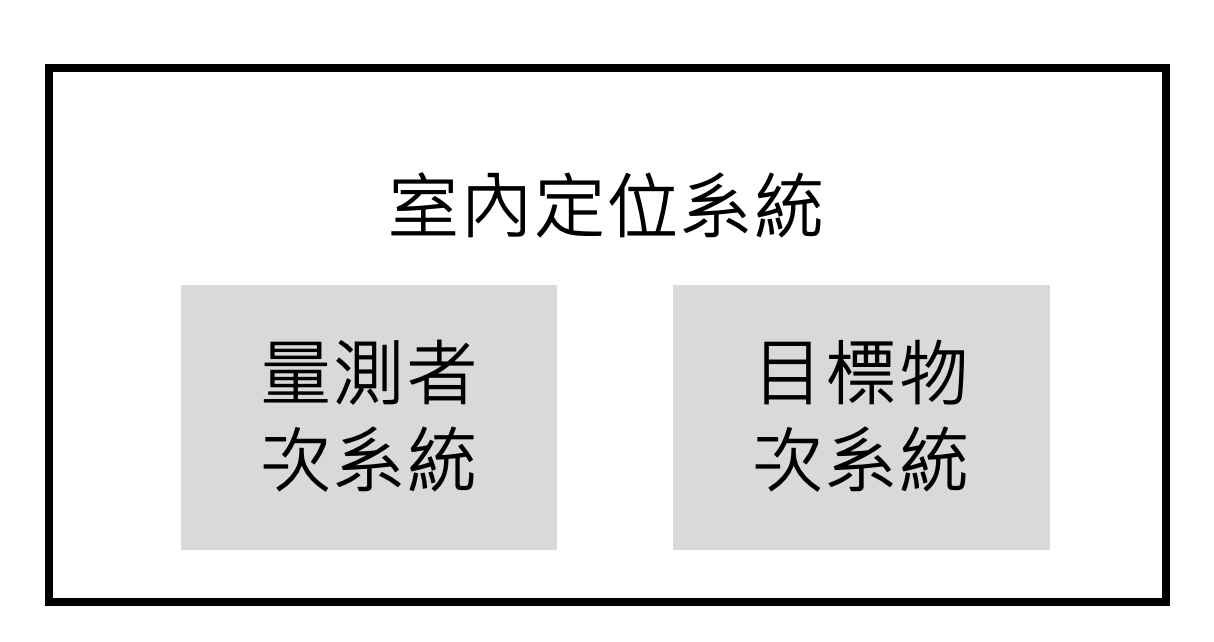
\includegraphics[width=7cm]{ch2pic/subsystem.png}
    \caption{室內定位系統與次系統}
    \label{pic:subsystem}
\end{figure}

\begin{figure}[htpb]
    \centering
    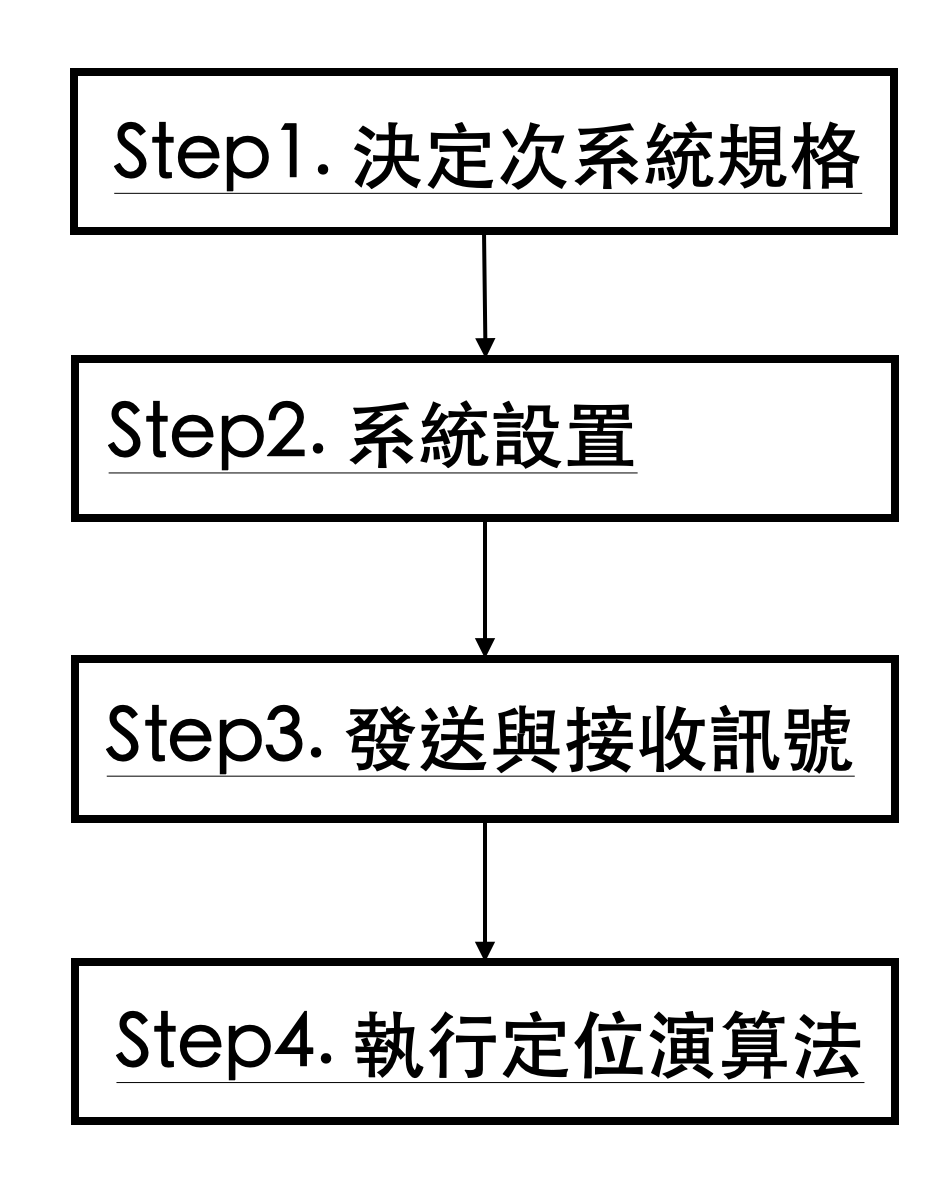
\includegraphics[width=5.5cm]{ch2pic/pos_flow.png}
    \caption{室內定位流程}
    \label{pic:pos_flow}
\end{figure}


室內定位系統架構如圖\ref{pic:subsystem},其由目標物次系統與量測者次系統組成,兩次系統各自擔任傳送訊號與皆收訊號兩任務。室內定位有非常多種硬體技術與後處理方法,無論何種技術,定位流程皆可以用圖\ref{pic:pos_flow}的步驟表示,依序為決定系統規格、系統設置、發送與接收訊號以及執行定位演算法四個步驟。決定次系統規格時,需分別設計量測者與目標物次系統,系統設置的步驟為將兩次系統放置於空間中,進行發送與接收訊號,藉由接收到的訊號進行最後的步驟:執行定位演算法。為方便後續敘述,本論文中都會以Step1.到Step4.描述定位流程中的四個步驟。

\begin{figure}[htpb]
    \centering
    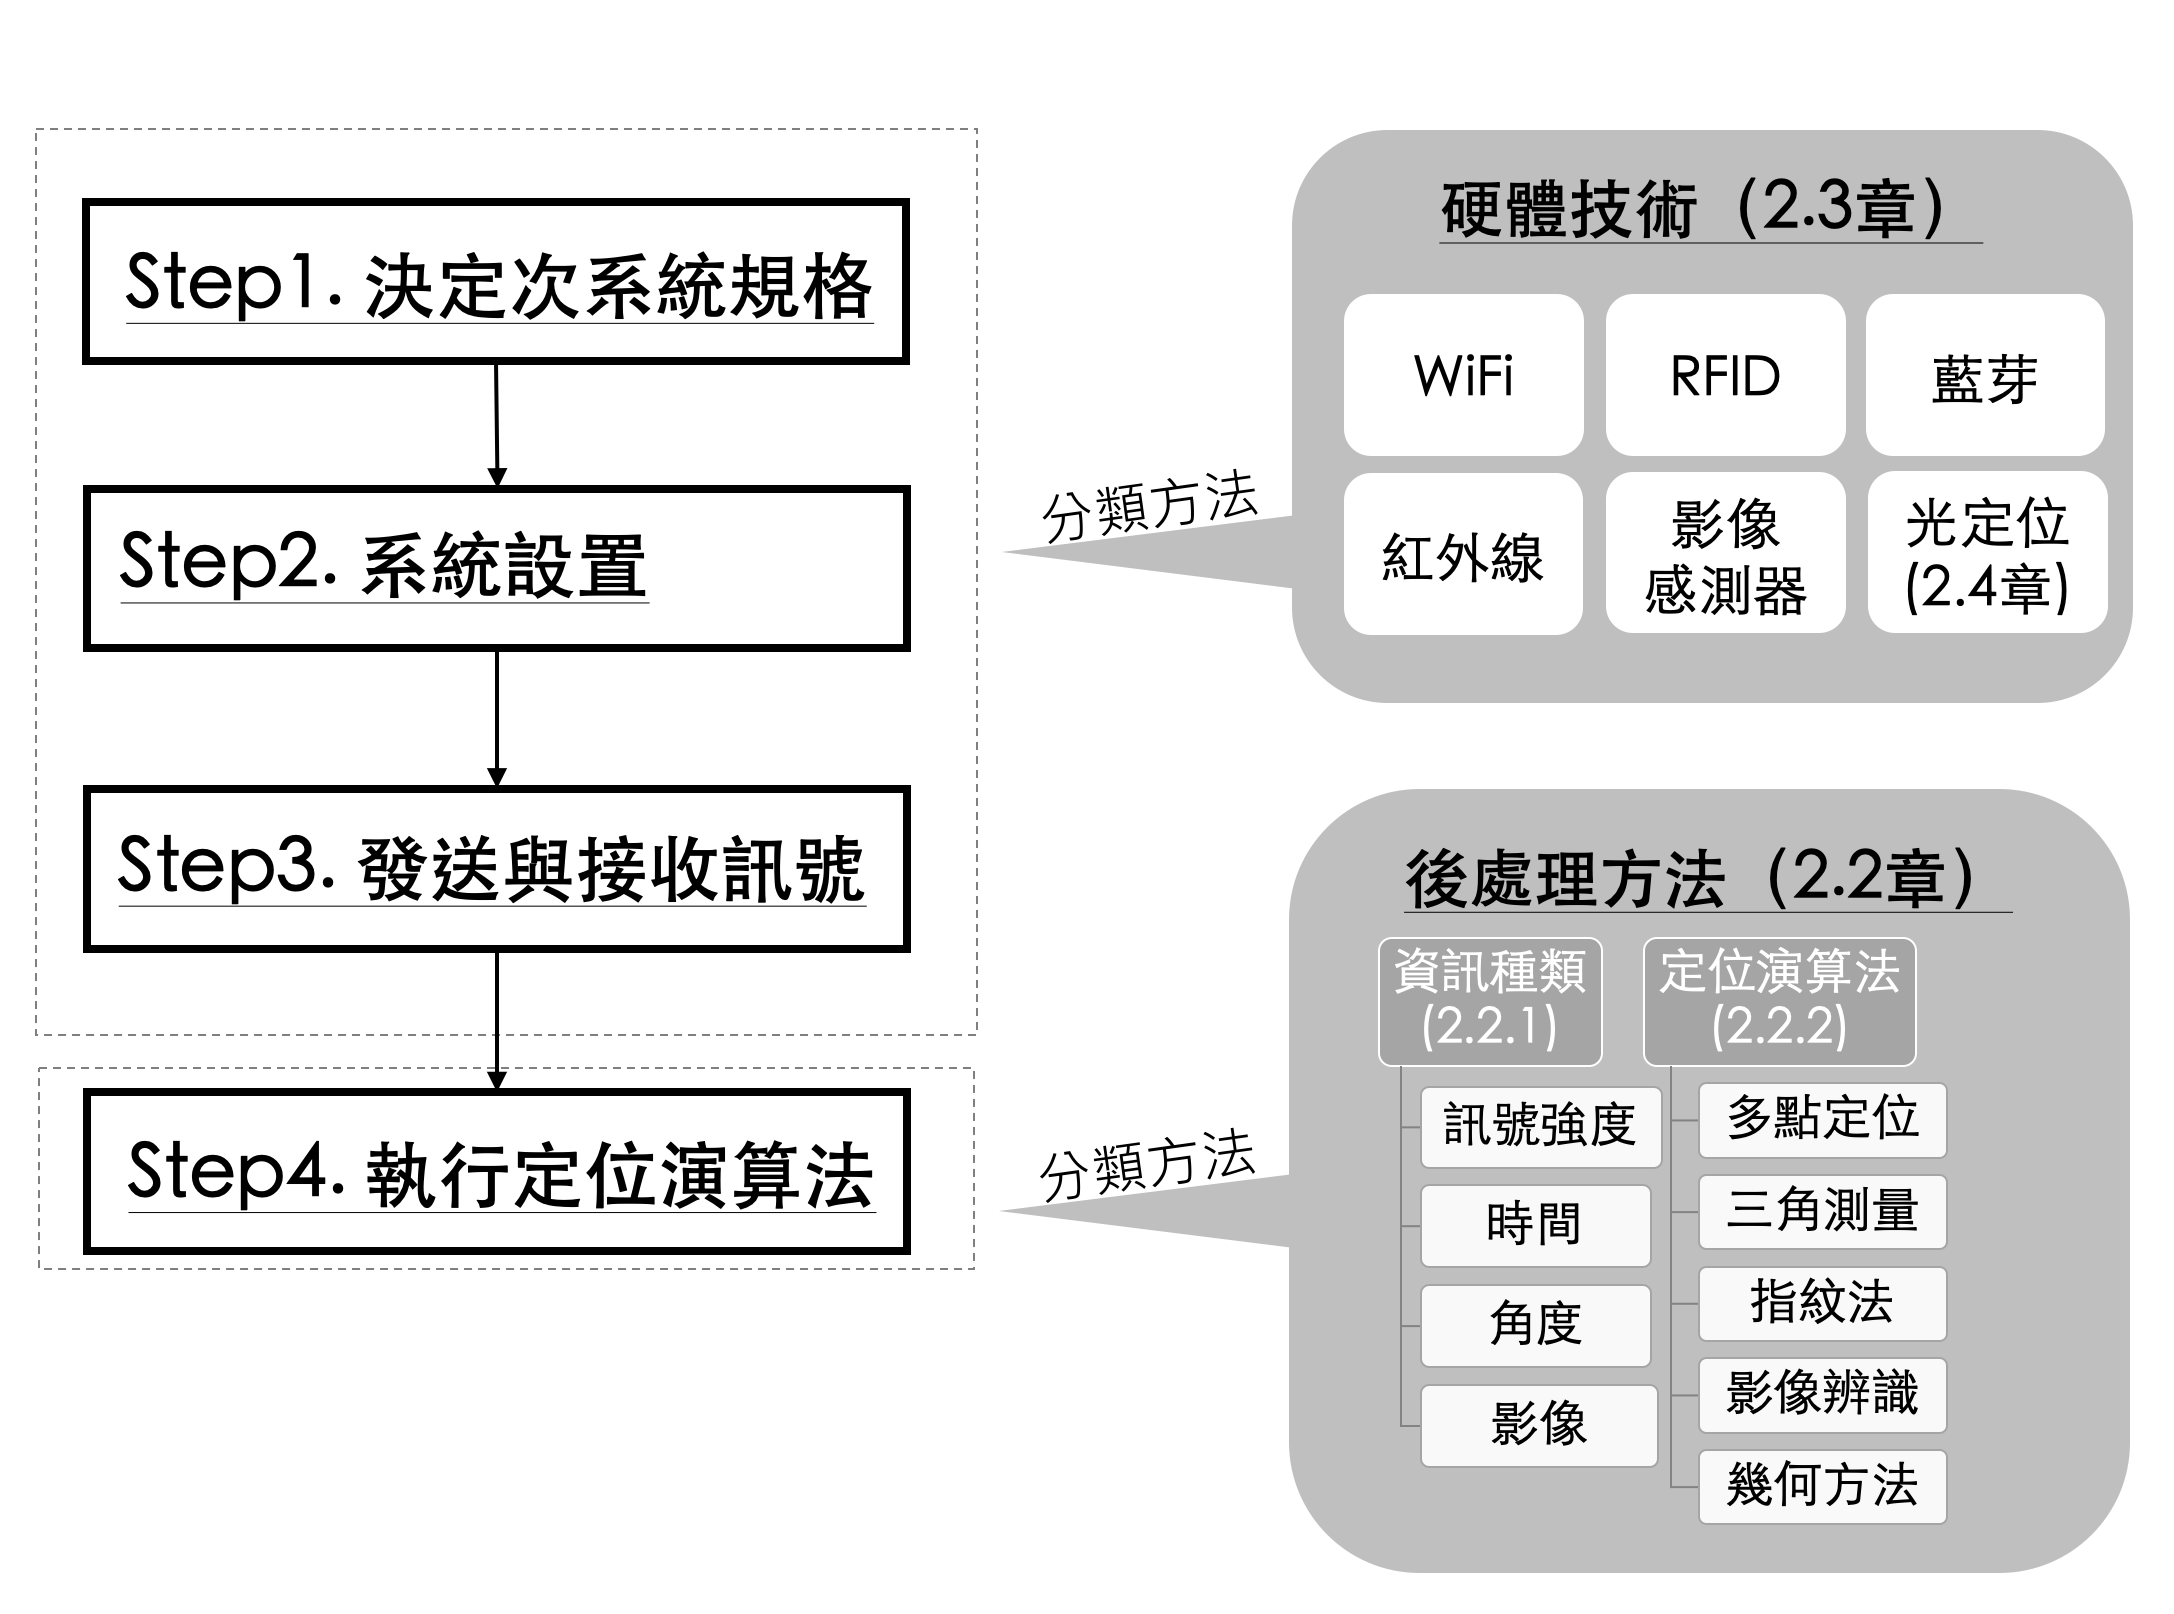
\includegraphics[width=13cm]{ch2pic/pos_category.png}
    \caption{室內定位分類}
    \label{pic:pos_category}
\end{figure}


本章節將依序於\ref{chp:relative}章先定義何謂相對定位,接著根據後處理方法與硬體技術分類介紹,分類方法如圖\ref{pic:pos_category},分別於\ref{chp:method}章介紹不同硬體技術,以及在\ref{chp:technique}章中介紹不同後處理方法,並根據\ref{chp:motivate}章中:硬體系統需為低能耗、可封裝成量測單位與目標物單位、進行單點對單點的定位的需求,聚焦在「LED與PD定位技術」,\ref{chp:LEDandPD}章便針對「LED與PD定位技術」進行深入探討,敘述此領域研究現況與困難,最後於\ref{chp:2_conclusion}章總結。


   





\section{相對定位定義}
\label{chp:relative}
% -(利用數學符號描述相對定位問題的定義(軌跡、時間等))

    
    在開始進入文獻探討之前,需先以數學定義何謂本論文所欲量測之「相對定位」。我們將取得相對位置的一方,也就是接收訊號的一方稱為量測者次系統,可由如光電二極體(Photodiode,以下簡稱PD)的感測器組成;而量測者次系統欲取得相對位置的特定物體,也就是發送訊號的一方,則稱為目標物次系統,如主動傳送訊號的發光二極體(Light Emitting Diode,以下簡稱LED)。

    \begin{figure}[htpb]
        \centering
        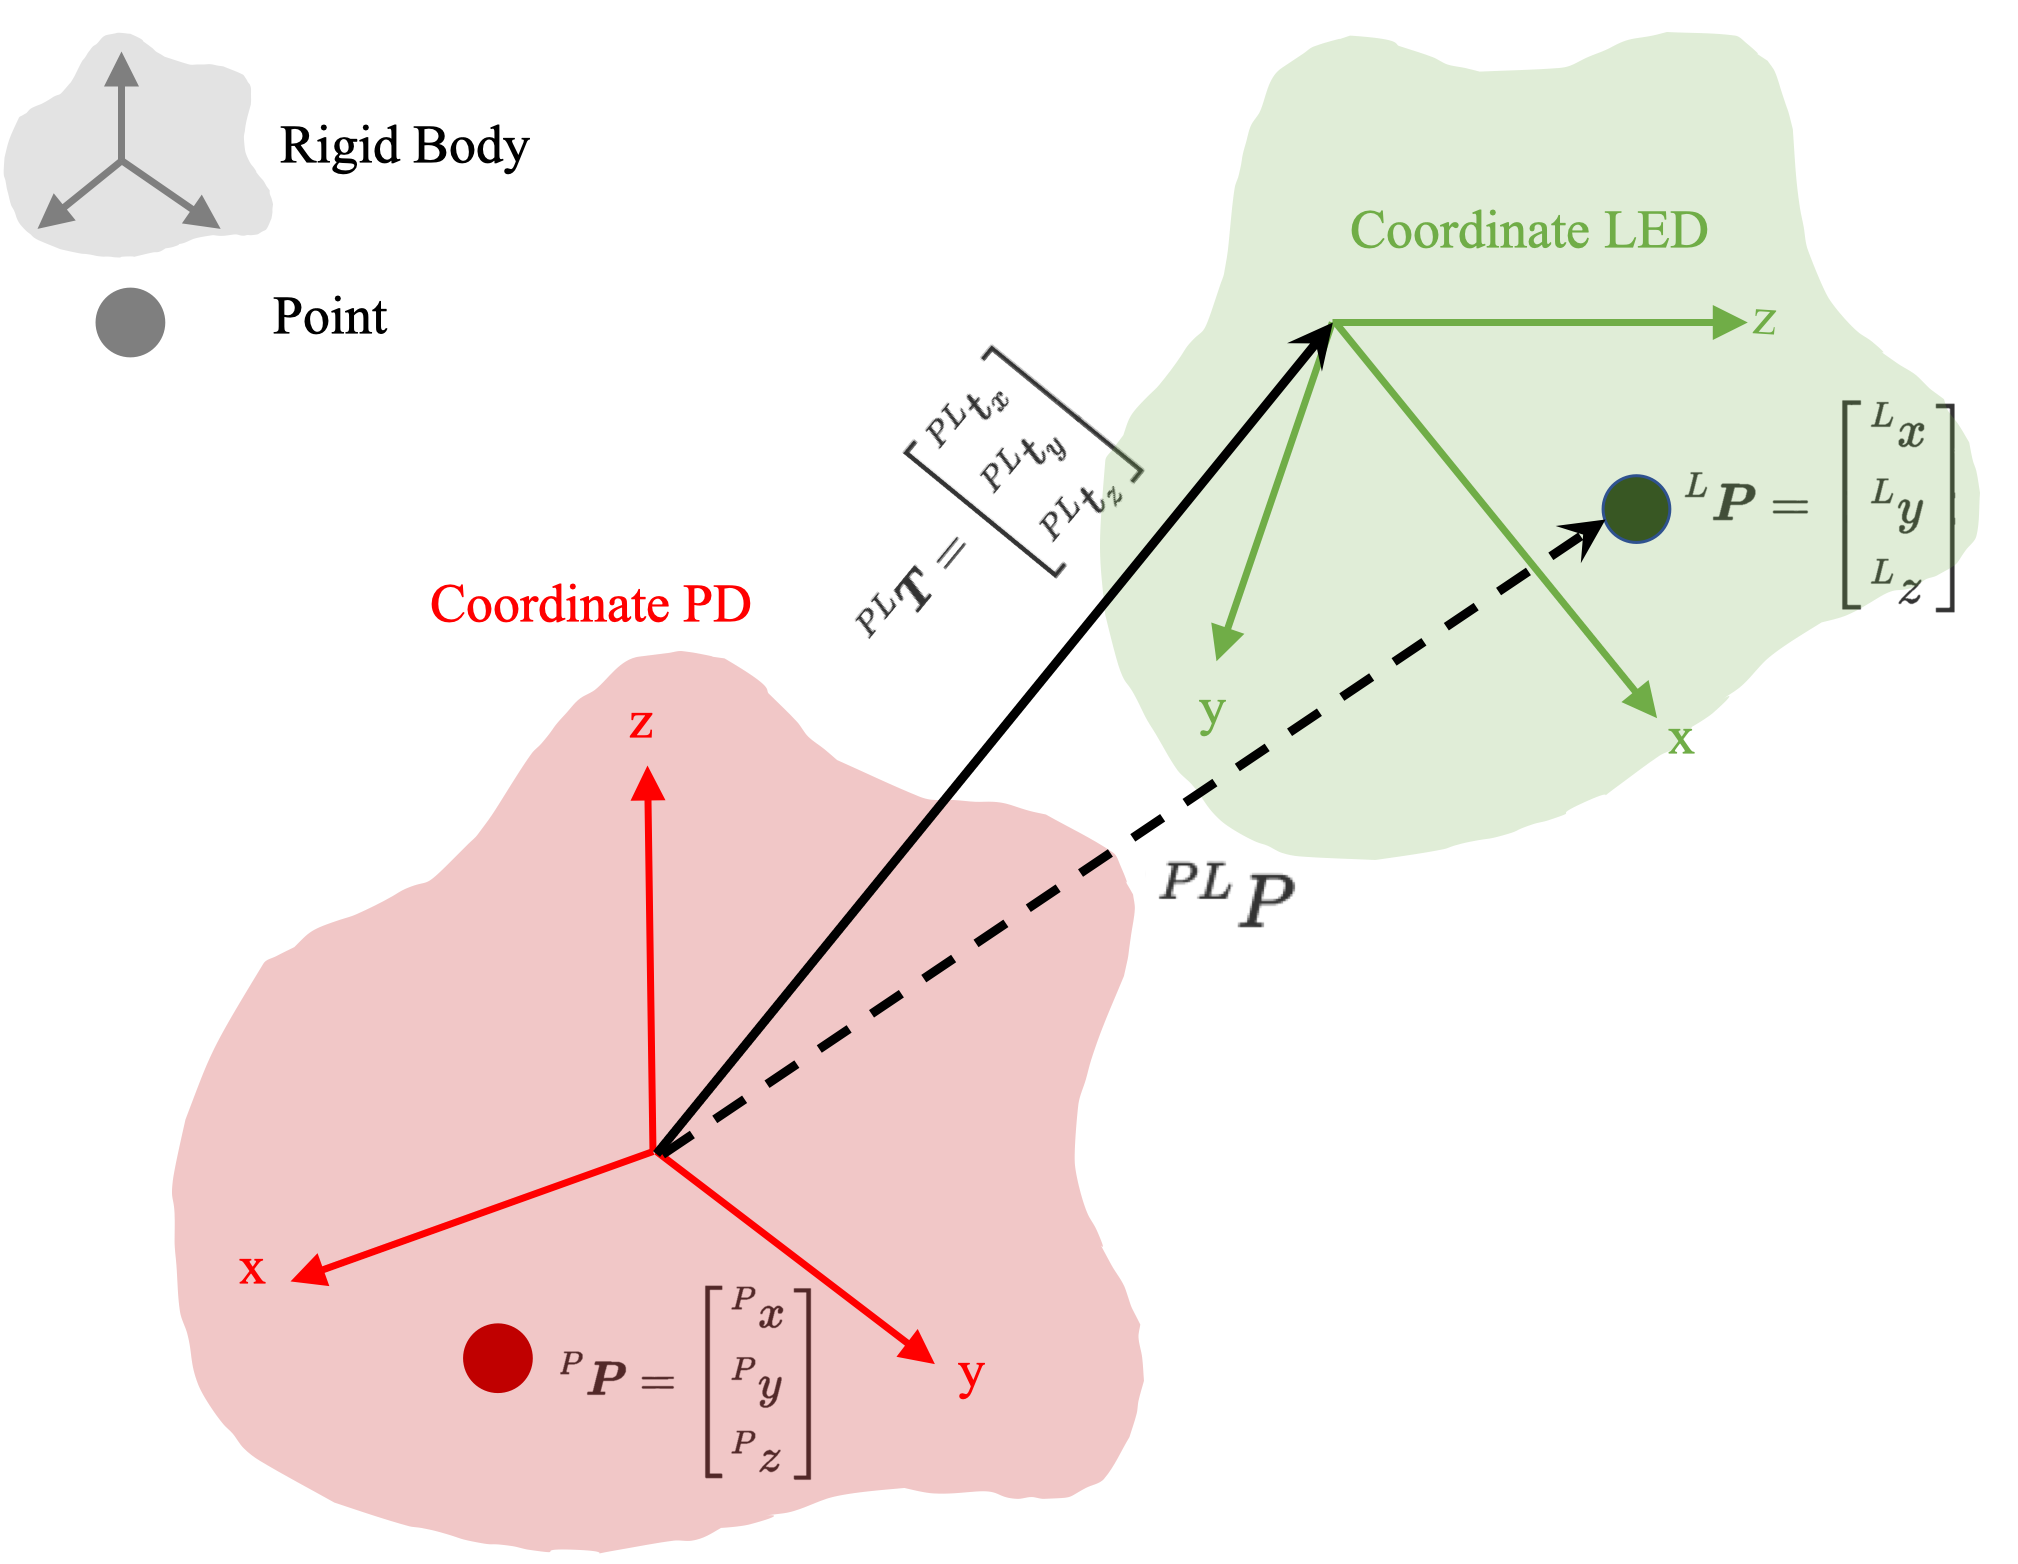
\includegraphics[width=11cm]{ch2pic/homo_trans.png}
        \caption{LED與PD次系統座標系及其相對關係}
        \label{pic:homo_trans}
    \end{figure}

    由於各次系統視為剛體,於Step1.決定次系統規格時,各感測器固定於該次系統硬體上。因此,可以將量測者次系統與目標物次系統,各自視為兩座標系如圖\ref{pic:homo_trans},兩次系統座標系在空間中各自有位置、旋轉的三個自由度,可以利用齊次座標轉換(Homogeneous Transformation)表示座標系之間的平移與旋轉如式\ref{eqn:homogeneous}。其中,我們以$\boldsymbol{P}$表示位置,左上標則表示定義於哪個座標系,以LED與PD系統為例,$^{L}\boldsymbol{P}$為LED的位置,而$^{PL}\boldsymbol{P}$為投影至PD座標系上的LED位置,描述投影的矩陣為齊次轉換矩陣$^{PL}\boldsymbol{H}$,左上標$PL$表示將LED座標系轉換至PD座標系,而$^{PL}\boldsymbol{T}$與$^{PL}\boldsymbol{Ro}$各自代表平移與旋轉的轉換矩陣,符號可參考符號列表(第\pageref{chp:symbol}頁)。

    
    
    
    
  

    \begin{equation}
        \label{eqn:homogeneous}
        \begin{aligned}
        {\left[\begin{array}{c}
        { }^{P L} \boldsymbol{P} \\
        1
        \end{array}\right]={ }^{P L} \boldsymbol{H}\left[\begin{array}{c}
        { }^{L} \boldsymbol{P} \\
        1
        \end{array}\right] } &=\left[\begin{array}{cc}
        { }^{P L} \boldsymbol{R} \boldsymbol{o} & { }^{P L} \boldsymbol{T} \\
        0 & 1
        \end{array}\right]\left[\begin{array}{c}
        { }^{L} \boldsymbol{P} \\
        1
        \end{array}\right] \\
        &=\left[\begin{array}{cccc}
        { }^{P L} \gamma_{11} & { }^{P L} \gamma_{12} & { }^{P L} \gamma_{13} & { }^{P L} {t}_{x} \\
        { }^{P L} \gamma_{21} & ^{P L } \gamma_{22} & { }^{P L} \gamma_{23} & { }^{P L} {t}_{y} \\
        { }^{P L} \gamma_{31} & ^{P L} \gamma_{32} & { }^{P L} \gamma_{33} & { }^{P L} {t}_{z} \\
        0 & 0 & 0 & 1
        \end{array}\right]\left[\begin{array}{c}
        { }^{L} {x} \\
        { }^{L} {y} \\
        { }^{L} z \\
        1
        \end{array}\right]
        \end{aligned}
    \end{equation}


    
    
   其中,兩座標系之間的平移關係$^{PL}\boldsymbol{T}$即為欲得到的相對位置資訊,共有三個自由度:$^{PL}\boldsymbol{T}=\left[\begin{array}{ccc}
    t_x &t_y&t_z
    \end{array}\right]^T$。以上座標皆以卡氏座標系(Cartesian Coordinate)表示,然而在定位中也常使用球座標系表示,讓定位以「距離$d$」與「方位($\alpha,\beta$)」呈現,較為直觀,可將方位想像成「看哪裡」,而距離則為「看多遠」。兩座標系之間的換算如式\ref{eqn:car2sph},球座標系中的位置$\boldsymbol{P}^{sph}$透過公式轉換為卡式座標系表示的$\boldsymbol{P}$:

   \begin{equation}
    \label{eqn:car2sph}
        \begin{aligned}
        \boldsymbol{P}^{sph}&=\left[\begin{array}{c}
            d\\\alpha\\\beta
            \end{array}\right] \\  
        \boldsymbol{P} &= \left[\begin{array}{c}
            x\\y\\z
            \end{array}\right]=
            \left[\begin{array}{c}
            d\sin\alpha\cos\beta \\
            d\sin\alpha\sin\beta\\
            d\cos\alpha
            \end{array}\right] 
    \end{aligned}
   \end{equation}

   在此需特別注意的是,LED座標系與PD座標系指的是「兩空間中移動的座標系」,而卡氏座標系與球座標系則是座標系的呈現方式;LED座標系可以用卡式座標系的$\left[\begin{array}{ccc}
    x &y&z
    \end{array}\right]^T$表達,也可以用球座標系的$\left[\begin{array}{ccc}
        d &\alpha&\beta
        \end{array}\right]^T$表示,PD座標系亦然。



\section{依後處理方法分類}
\label{chp:method}

    
    根據圖\ref{pic:pos_category}中所示,定位分類可以由使用的硬體技術與後處理方法分類,為了在介紹硬體技術時可以參照各自硬體使用的後處理方法,我們先於本段落介紹不同的後處理方法,於\ref{chp:technique}中再介紹不同的硬體技術。

    後處理方法可以分類成兩部分如圖\ref{pic:pos_category}:第一個分類標準是資訊種類的不同,也就是室內定位的硬體在接收訊號時,量測者次系統所接收的資訊種類;第二種分類標準則是在接收資訊後,如何利用資訊計算出相對位置,屬於定位演算法的部分。而資訊種類與後處理演算法並不能任意搭配,各資訊種類都是會有合適的後處理演算法如圖\ref{pic:method_sort},以下依續介紹不同的資訊種類與後處理演算法。

    \begin{figure}[htpb]
        \centering
        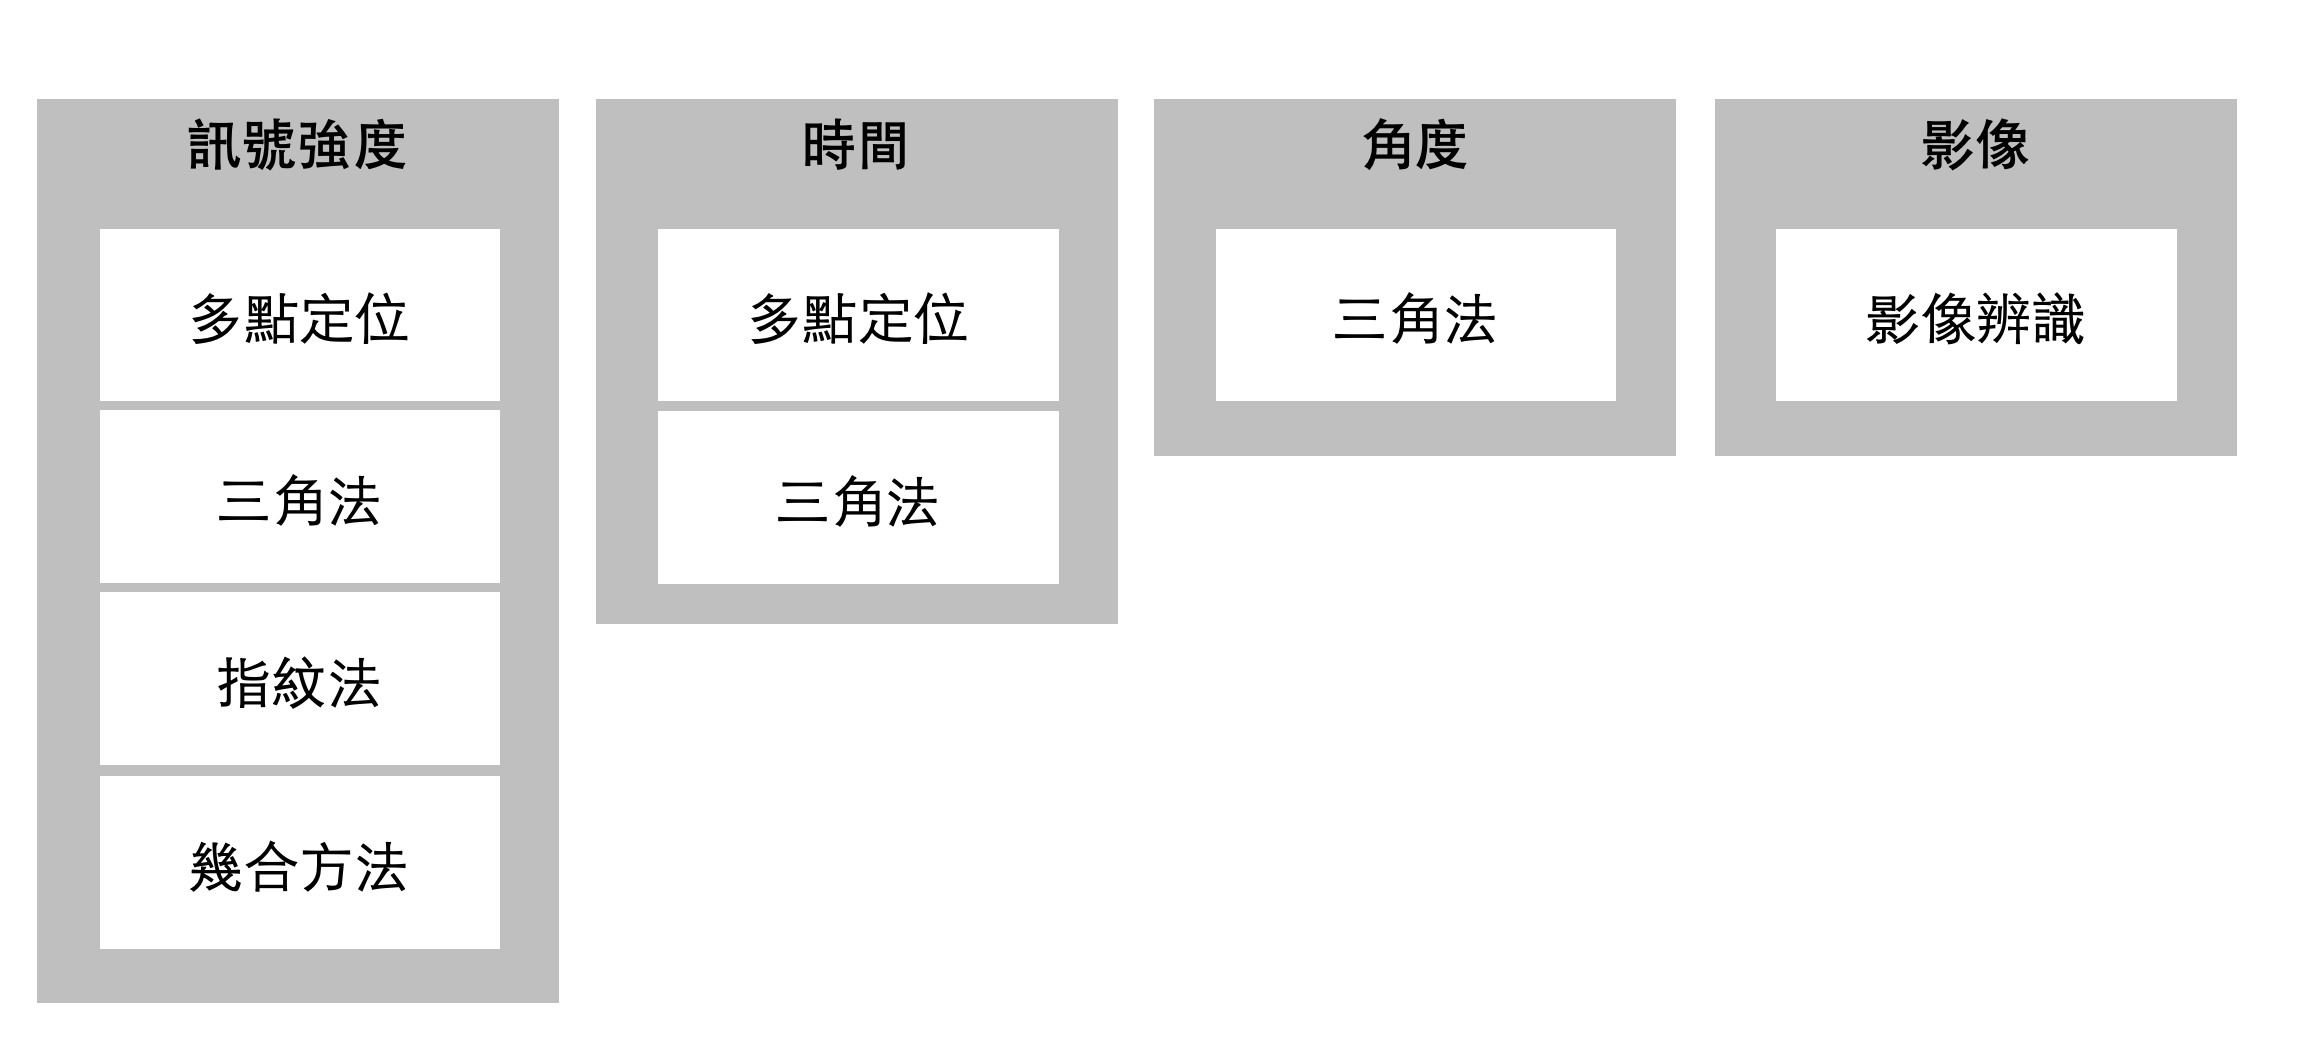
\includegraphics[width=15cm]{ch2pic/method_sort.png}
        \caption{資訊種類與演算法之間的關聯(參考\cite{survey_light2018})}
        \label{pic:method_sort}
    \end{figure}
    
    \subsection{資訊種類}

    常見的訊號種類包含訊號強度(Received Signal Strength,簡寫RSS)、時間、角度與影像。訊號強度為最常見的資訊種類\cite{survey_indoor2018},使用的是該硬體所接收到的訊號強度,而利用訊號強度的演算法也十分多樣,包含多點定位、三角法、指紋法等,詳述於\ref{chp:method-algorithm}章。

    時間資訊種類則是硬體利用訊號之間的時間差量測距離的方法,常見使用的技術為紅外線,紅外線可以利用訊號傳送到不同接收子的時間差,判斷出之間的距離。若要利用時間資訊,在各硬體之間則需要將時間同步,在實作上為一大挑戰\cite{survey_indoor2014}。

    若獲取的是角度資訊,基本上演算法便會搭配三角法,綜合多個接收子的角度獲得相對位置。影像則屬於影性感測器(Image Sensor)獨有,且搭配的定位演算法為影像辨識。


    \subsection{定位演算法}
    \label{chp:method-algorithm}

    常見的演算法則包含多點定位、三角測量、指紋法、影像辨識以及幾何方法,以下條列依續介紹不同定位演算法。

    \begin{description}
        \item[- 多點定位(Multilateration)]\hfill 
        
        \qquad
        多點定位如圖\ref{pic:multilateration}所示,需在環境中建立多個參考點並固定位置,量測目標物與多個參考點之間的距離,進而以各參考點為中心、距離為半徑畫圓求交點。

        \begin{figure}[htpb]
            \centering
            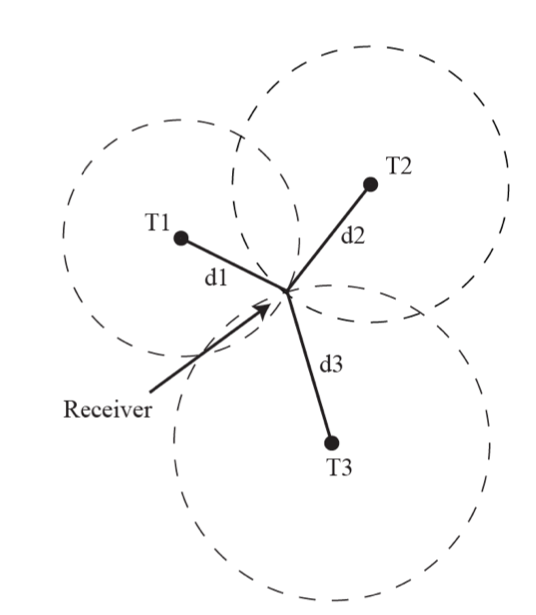
\includegraphics[width=6cm]{ch2pic/multilateration.png}
            \caption{多點定位法\cite{survey_light2020}}
            \label{pic:multilateration}
        \end{figure}
    
        \item[- 三角測量(Triangulation)] \hfill 
        
        \qquad
        三角測量法如圖\ref{pic:triangulation}所示,需要在環境中建立多個參考點,藉由量測目標物與各參考點之間的角度關係,推算目標物位置。
        \begin{figure}[htpb]
            \centering
            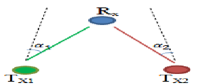
\includegraphics[width=9cm]{ch2pic/triangulation.png}
            \caption{三角測量法\cite{survey_light2018}}
            \label{pic:triangulation}
        \end{figure}
        
        \item[- 指紋法(Fingerprinting)] \hfill 
        
        \qquad
        指紋法的流程圖如圖\ref{pic:fingerprinting},在環境中建立多個參考點,在實際進行測量前,需進行事先測量訓練的階段,此階段中需將目標物在環境中移動,蒐集大量訊號數據庫。量測階段則藉由接收訊號與訓練階段所建立的數據庫參照,尋找最有可能存在的位置\cite{survey_light2020},近年則是有許多以機器學習方法增加此演算法的精確度。
        \begin{figure}[htpb]
            \centering
            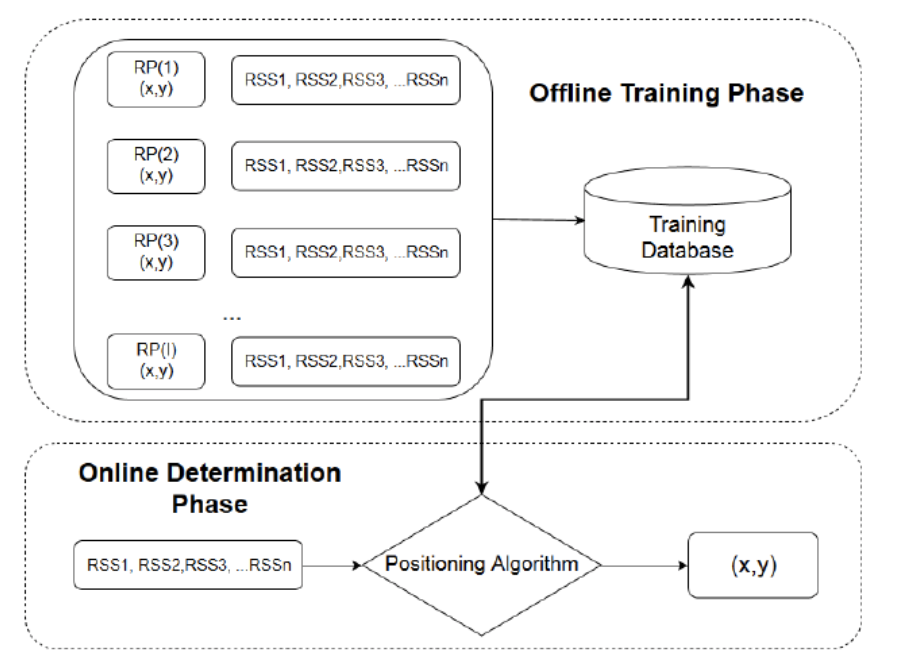
\includegraphics[width=13cm]{ch2pic/fingerprinting.png}
            \caption{指紋法流程圖\cite{pic:fingerprinting}}
            \label{pic:fingerprinting}
        \end{figure}
        
        \item[- 影像辨識]\hfill 
        
        \qquad
    如圖\ref{pic:image_processing},三維空間中的物體透過相機拍攝成為二維的影像時,為三維空間投影至二維影像平面上的幾何轉換。反之,利用影像辨識求解相對位置時,則是試圖將二維影像中的特徵點比對、轉換回三維空間中,利用PnP演算法(Perspective-n-Point)解出目標物相對影像感測器座標系的位置與方位\cite{pic:image_processing}。
        
        \begin{figure}[htpb]
            \centering
            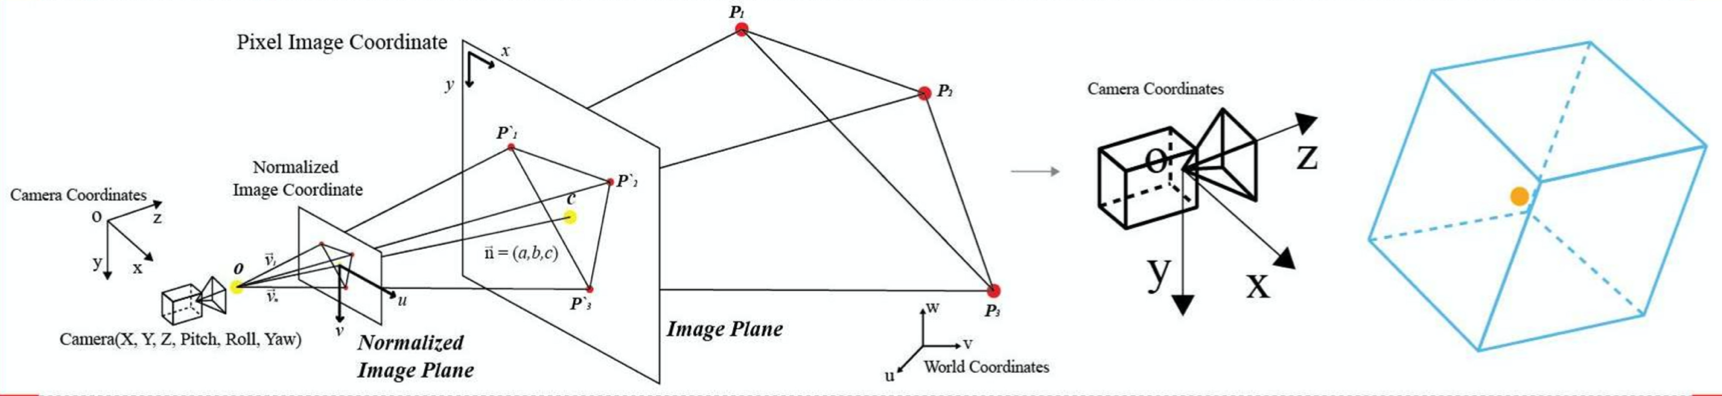
\includegraphics[width=15cm]{ch2pic/image_processing.png}
            \caption{影像辨識示意圖\cite{pic:image_processing}}
            \label{pic:image_processing}
        \end{figure}
        
        \qquad
        為了使辨識過程中辨識特徵點的難度降低,通常會設計特徵明顯的標記,例如常見OpenCV中的ArUco標記如圖\ref{pic:aruco},利用其快速得辨識ID以及距離、方位等資訊。
        
        \begin{figure}[htpb]
            \centering
            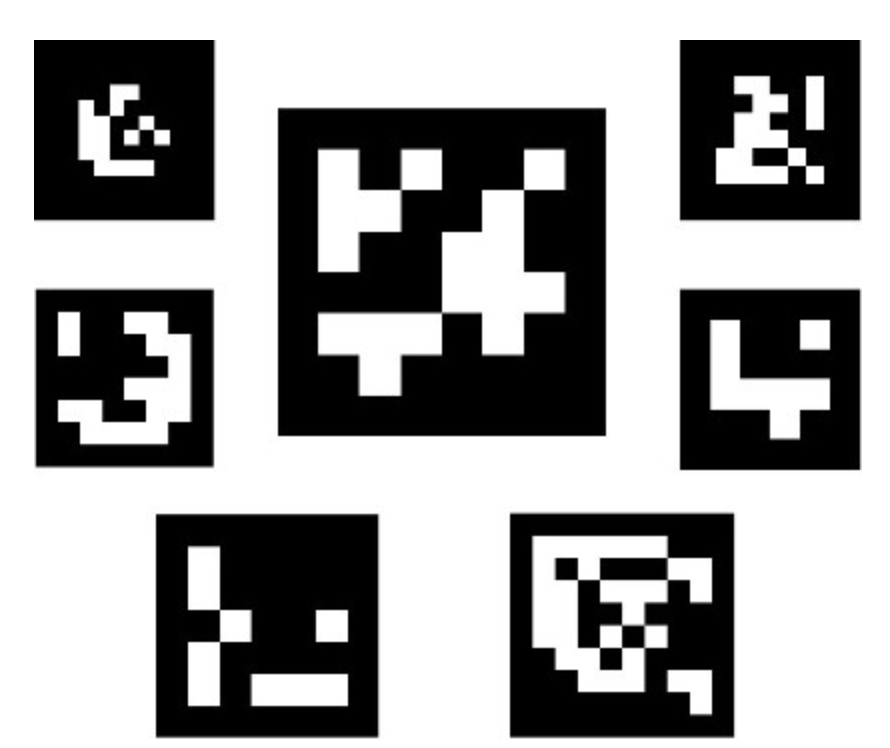
\includegraphics[width=5cm]{ch2pic/aruco.png}
            \caption{ArUco標記例子\cite{pic:aruco}}
            \label{pic:aruco}
        \end{figure}
        
        \item[- 幾何方法] \hfill 
        
        \qquad
        此類方法常見於LED與PD的定位方法,並沒有一通用的分類名稱,方法利用PD接收訊號強度與距離、出入社角度皆有關,因此需綜合角度與距離資訊,透過兩次系統間訊號強度與相對位置之間的幾何關係推算相對位置\cite{survey_light2020},詳述於\ref{chp:model}。
        
        \item[- 其他]\hfill 
        
        \qquad
        常見的其他種類演算法多會使用混合系統(Hybrid System)\cite{survey_indoor2018},除了使用量測距離、角度等位置資訊的感測器,多與其他量測姿態、速度的感測器結合使用,如動作捕捉(Motion Capture)領域中使用慣性量測單元(Inertial Measurement Unit,簡稱IMU)量測點的移動軌跡。

    \end{description}

    \subsection{小結}

    \ref{chp:motivate}章所總結對系統的需求中,演算法在單點對單點的定位上影響顯著,在常見演算法中,僅有影像辨識與幾何方法能夠達到單點對單點的定位,符合本研究需求。這兩種定位演算法,都是利用目標物與量測者之間的幾何關係來進行定位的判斷,能夠適應不同環境、不同系統設置位置的改變,做到「單位對單位的定位」。相較起來,多點定位、三角法、指紋法都需要多個固定的參考點以量測定位,屬於環境對單點的定位,無法符合可攜式單位與易於安裝單元的需求。




\section{依硬體技術分類}
\label{chp:technique}

    室內定位所使用的硬體技術(Technique)一樣十分多樣,其中,非電磁波段的定位主要為超聲波,應用訊號發射與接收之間的時間差,推算與目標物之間的距離。然而該技術受溫度影響,且對目標物的辨識能力不佳,因此目前著重在自駕車與載具中障礙物的有無偵測上\cite{survey_ultrasonic},並不符合研究目標,所以以下章節聚焦在電磁波段內的定位進行分析。

    電磁波段內有許多不同現今受到關注的量測技術,電磁波段內常見的技術於\ref{chp:intro}章內有簡單介紹,而電磁波以光速傳播,擁有高傳播速度與不受介質溫度與濕度影響的特性,減少可能對量測訊號造成影響的因素。

    \begin{figure}[htpb]
        \centering
        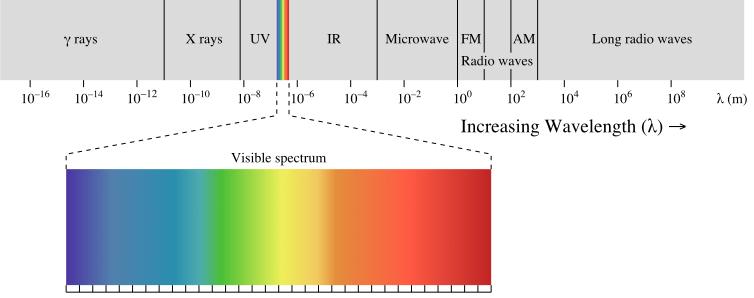
\includegraphics[width=15cm]{ch2pic/electro_spectrum.png}
        \caption{電磁波頻譜度\cite{Spectrum}}
        \label{pic:spectrum}
    \end{figure}

    我們由電磁波的頻率切入進行不同硬體技術的分類,頻譜圖如圖\ref{pic:spectrum},能夠用於定位的波段為頻率低於約790THz的波段,因為電磁波頻率越高所含能量越高使高頻波段對人體有害,因此高於此波段的電磁波具有過高能量,導致此波段中的X光、紫外線、伽瑪射線無法使用於日常應用,不予考慮。

    對人體無害的波段則分為兩部分探討:\ref{chp:radio}章探討頻率低於300GHz的低頻波段\cite{book_electromagnetic},使用此波段的硬體技術包含Wifi、藍芽、RFID;而在\ref{chp:light}章介紹頻率介於790THz與300GHz之間的光波段,此波段的硬體技術包含紅外線、可見光定位以及影像感測器定位。以下章節便以圖\ref{pic:electro_sort}為架構依序介紹。


    \begin{figure}[htpb]
        \centering
        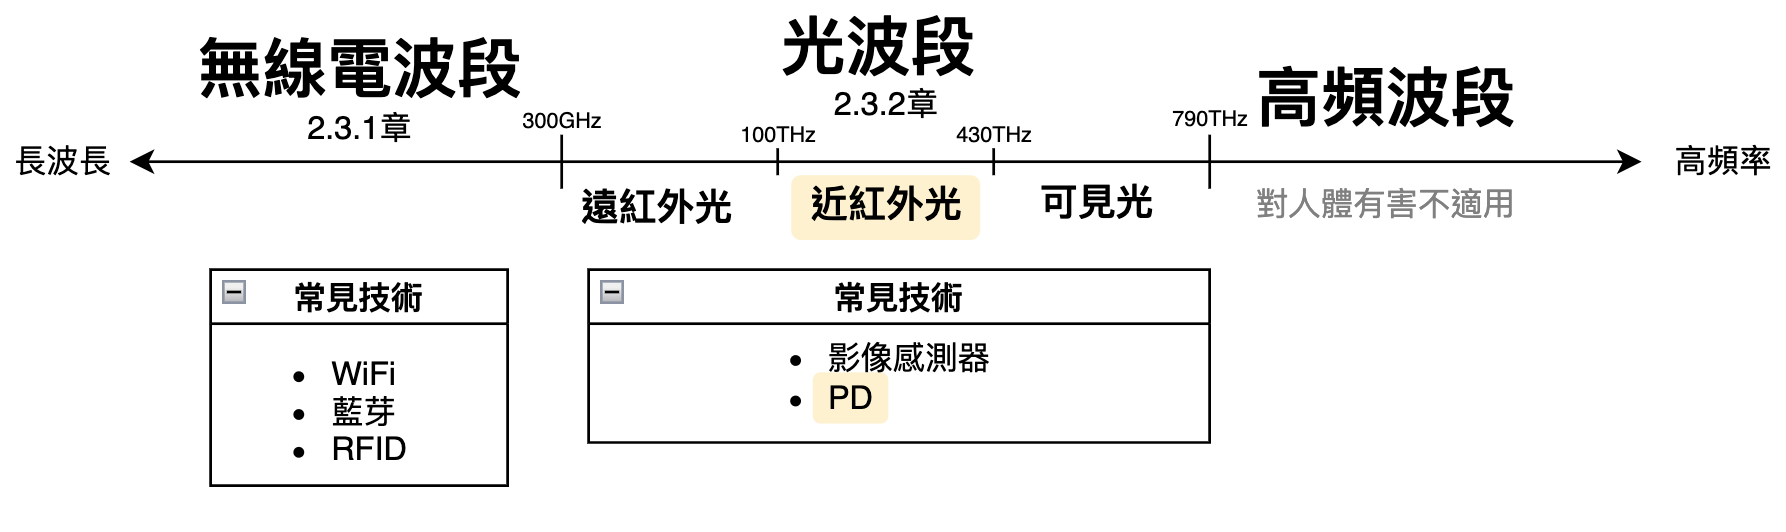
\includegraphics[width=15cm]{ch2pic/electro_sort.png}
        \caption{以電磁波頻率分類硬體技術}
        \label{pic:electro_sort}
    \end{figure}

    











    \subsection{無線電波段定位}
    \label{chp:radio}
    
        低頻波段也就是俗稱的無線電波(Radio Waves),應用發展歷史長,對於可使用的頻率有嚴格規範,台灣由國家通訊委員會訂定嚴格的可使用頻率波段\cite{rf_law},保證軍警、醫療、廣播等的傳播需求。常見使用無線電波段的定位技術包含WiFi與藍芽裝置,這兩種技術普遍於室內許多設施與手機,除此之外也包含技術較新的RFID定位技術。
    
        無線電波的主要特色包含可穿透大多障礙物,因此可用於跨房間非可視範圍(NLoS)的定位\cite{survey_indoor2018},增加了應用場域,然而也大大提升了訊號處理的難度,使感測器難以辨別訊號衰減原因為距離、角度、亦或是障礙物,因此選擇非可視範圍內定位即捨棄精度。除此之外,無線電波的傳遞距離很長,定位範圍較廣,WiFi甚至可達距離50公尺的定位\cite{survey_indoor2014}。所需面對的誤差處理包含電磁干擾、同頻道干擾(Co-channel Interference)、受障礙物與金屬影響的穿透效果等。

        至於無線電波段所使用的定位演算法,大多系統皆是利用指紋法、多點定位、三角法的方式,共通點是都需要多個參考點,事先的安裝與校正步驟相較複雜,應用場域著重在固定場域,而精度多為公尺量級。
    
        舉例來說,此波段大多應用在固定的場域中,常見的後處理方法包含指紋法的,或是利用大量的感測器與訊號發射器來判斷定位\cite{survey_rfid},系統設置皆與圖\ref{pic:rfid_system}相似,差異於感測器擺放的方法以及演算法。其中,最經典的LANDMARC例子\cite{landmarc}的環境如圖\ref{pic:landmarc}所示,也是將感測器散布於環境中。

        

        \begin{figure}[htpb]
            \centering
            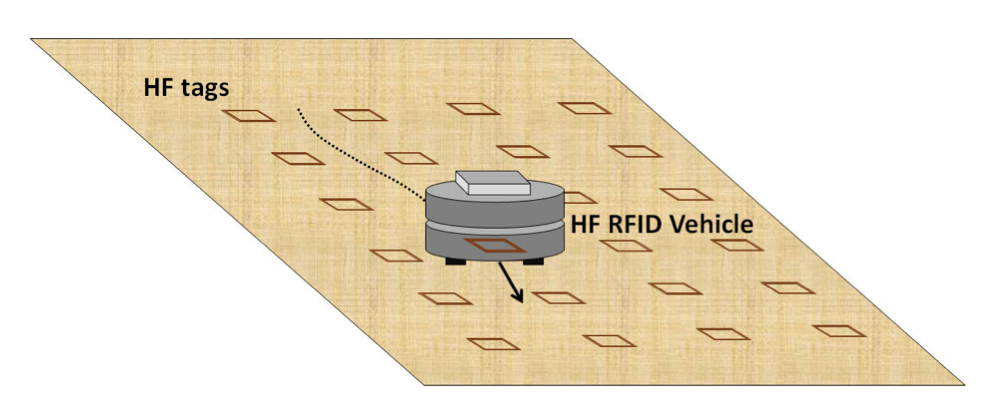
\includegraphics[width=6cm]{ch2pic/rfid_system.png}
            \caption{RFID定位系統示意\cite{survey_rfid}}
            \label{pic:rfid_system}
        \end{figure}

        \begin{figure}[htpb]
            \centering
            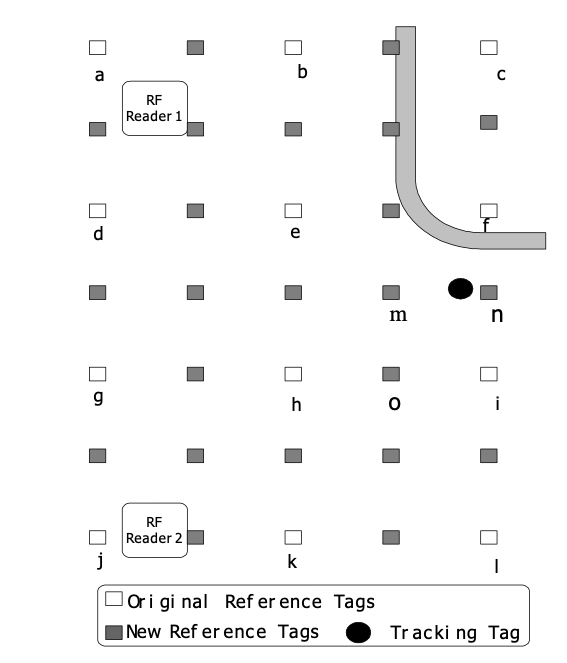
\includegraphics[width=8cm]{ch2pic/landmarc.png}
            \caption{LANDMARC系統環境\cite{landmarc}}
            \label{pic:landmarc}
        \end{figure}

        無線電波段也有少數例用\ref{chp:method-algorithm}章中所提到的三角法,如\cite{case:rfid_1to1}研究(圖\ref{pic:rfid_1to1}),例用RFID天線所接收到的訊號強度與入射角度的關係,在載具上放置兩天線,而擺放角度有90度的差異,藉由RFID發射器傳送訊號至天線的入射角度不同,計算出目標物的方位。此文獻提出了一種一對一定位的方法,然而其只能解出目標物的方位,也就是二維定位,並不包含距離。除此之外,由於可穿透障礙物的特色,隨著測試環境中添加障礙物、人、移動物品,皆會影響到訊號,造成誤差。

        \begin{figure}[htpb]
            \centering
            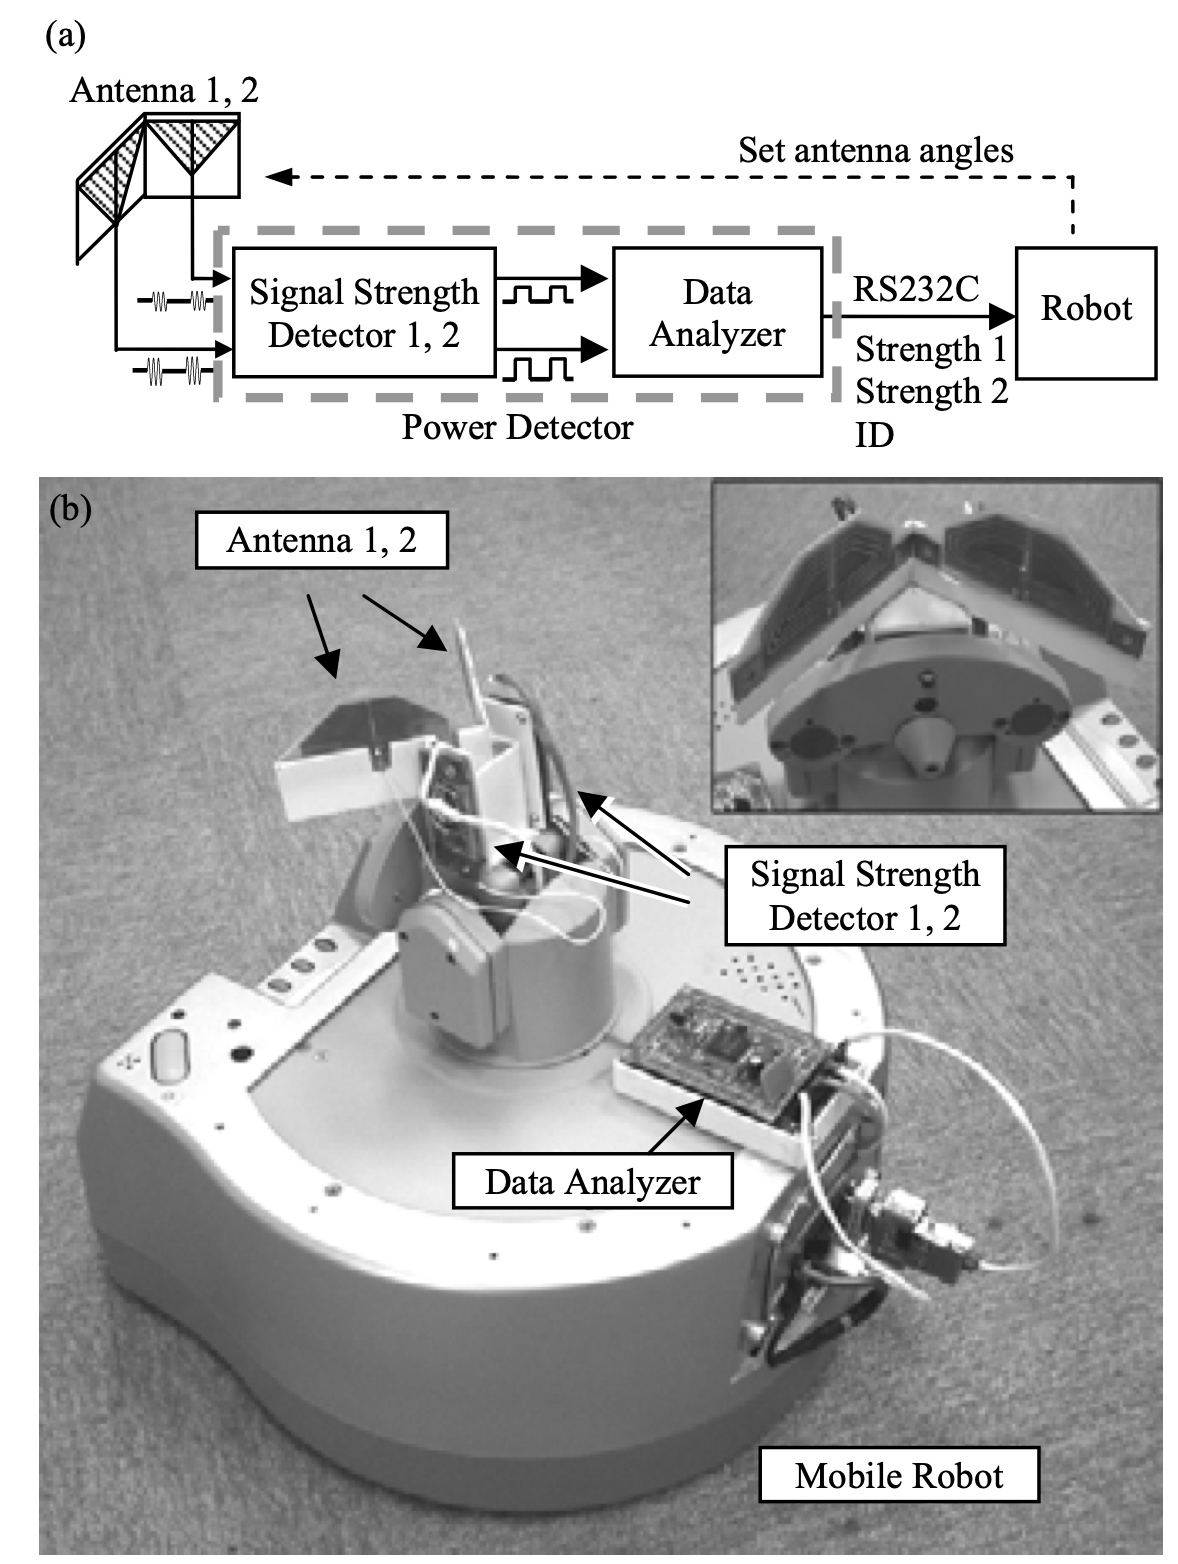
\includegraphics[width=8cm]{ch2pic/rfid_1to1.png}
           \caption{利用三角法定位的RFID系統\cite{case:rfid_1to1}(a)系統架構 (b)載具實驗}
            \label{pic:rfid_1to1}
        \end{figure}
        
        最後總結無線電波段的特色:此波段常使用於傳輸訊號的功能上,因此有成熟的編碼與解碼技術,能夠輕易達到辨識目標物的功能;而能夠穿透障礙物的以及傳輸距離長的特性,使得應用範圍大又不受視線範圍拘束;然而精度相較低,因此大多仰賴多個參考點或是事前建立數據庫的指紋法,應用的靈活度降低,較不符合本研究目標,因此著重在\ref{chp:light}章中的光波段定位。

       



       


        \subsection{光波段定位}
        \label{chp:light}
            
            光波段的定位發展近幾年來十分顯著,主要原因為光學硬體上的進步,促使光通訊(Light Communication)的發展,使發光與感光元件具有傳播ID、訊息等資訊的能力,因此光通訊與光定位便於近年得到研究關注\cite{survey_light2018}。光通訊流程如圖\ref{pic:vlc_flow}所示,利用驅動器調控光源的閃爍頻率、發光強度,來達到編碼的效果,最常見的編碼方式即為關閉調控(On-Off Keying,以下簡稱OOK),藉由開關光源傳送一段二進制訊號;感測器多以PD接收,接收後透過解碼取得資訊\cite{pic:vlc}。
            \begin{figure}[htpb]
                \centering
                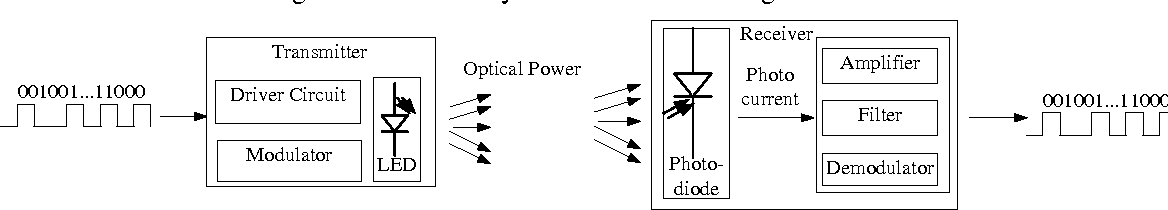
\includegraphics[width=15cm]{ch2pic/vlc_flow.png}
                \caption{光通訊流程圖\cite{pic:vlc}}
                \label{pic:vlc_flow}
            \end{figure}

            光波段在應用場域有一優勢,其可應用於無線電波限制的場域,如機場與醫院等特殊醫療場域\cite{case:vlc_mobile},且在如今無線電波訊號充斥環境的狀況下,而光波段即提供一替代方案。即使無線電波擁有很廣頻率選擇,然而隨著現今通訊需求的提升,無線電波段已被證實有塞車的狀況出現,光通訊便是一應對此困境之解決方法。
            
            
            再來,光波段無法穿透障礙物,僅能進行可視範圍內(Line-of-Sight,以下簡稱LoS)的定位,捨棄廣域的定位以獲得較為單純的量測數據。此特性同時增加光通訊的安全性以及穩定度,著重針對可視範圍進行通訊與定位,不受多餘訊號的干擾\cite{vlc_adv}。例如載具運行時,僅需著重分析於周遭的其他物體,位於隔壁房間的物體毫不重要,因此LoS通訊定位可忽略不重要的資訊,增加處理速度與訊號穩定度。即便如此,僅能進行LoS定位也限制了能夠量測的範圍,在環境阻擋物較多的情境會擋住光訊號的傳輸,使其無法進行定位。


            除此之外,電磁波有一特性為:波長愈短可達到的量測精度愈高,且感測器與訊號發射器的硬體大小也愈小,例如市售便宜常見的光波段感測器如PD感光二極體尺寸量級為mm或以下\cite{datasheet:led_sfh4545}且能耗低,相較之下使用低頻波段的RFID感測器常見量級為較大的cm\cite{datasheet:rfid_tag}。因此,選擇波長較短的光波段相較無線電波段具有硬體上的優勢。

            \begin{table}[htpb]
                \centering
                \caption{無線電波段與光波段的比較}
                \label{pic:method_compare}
                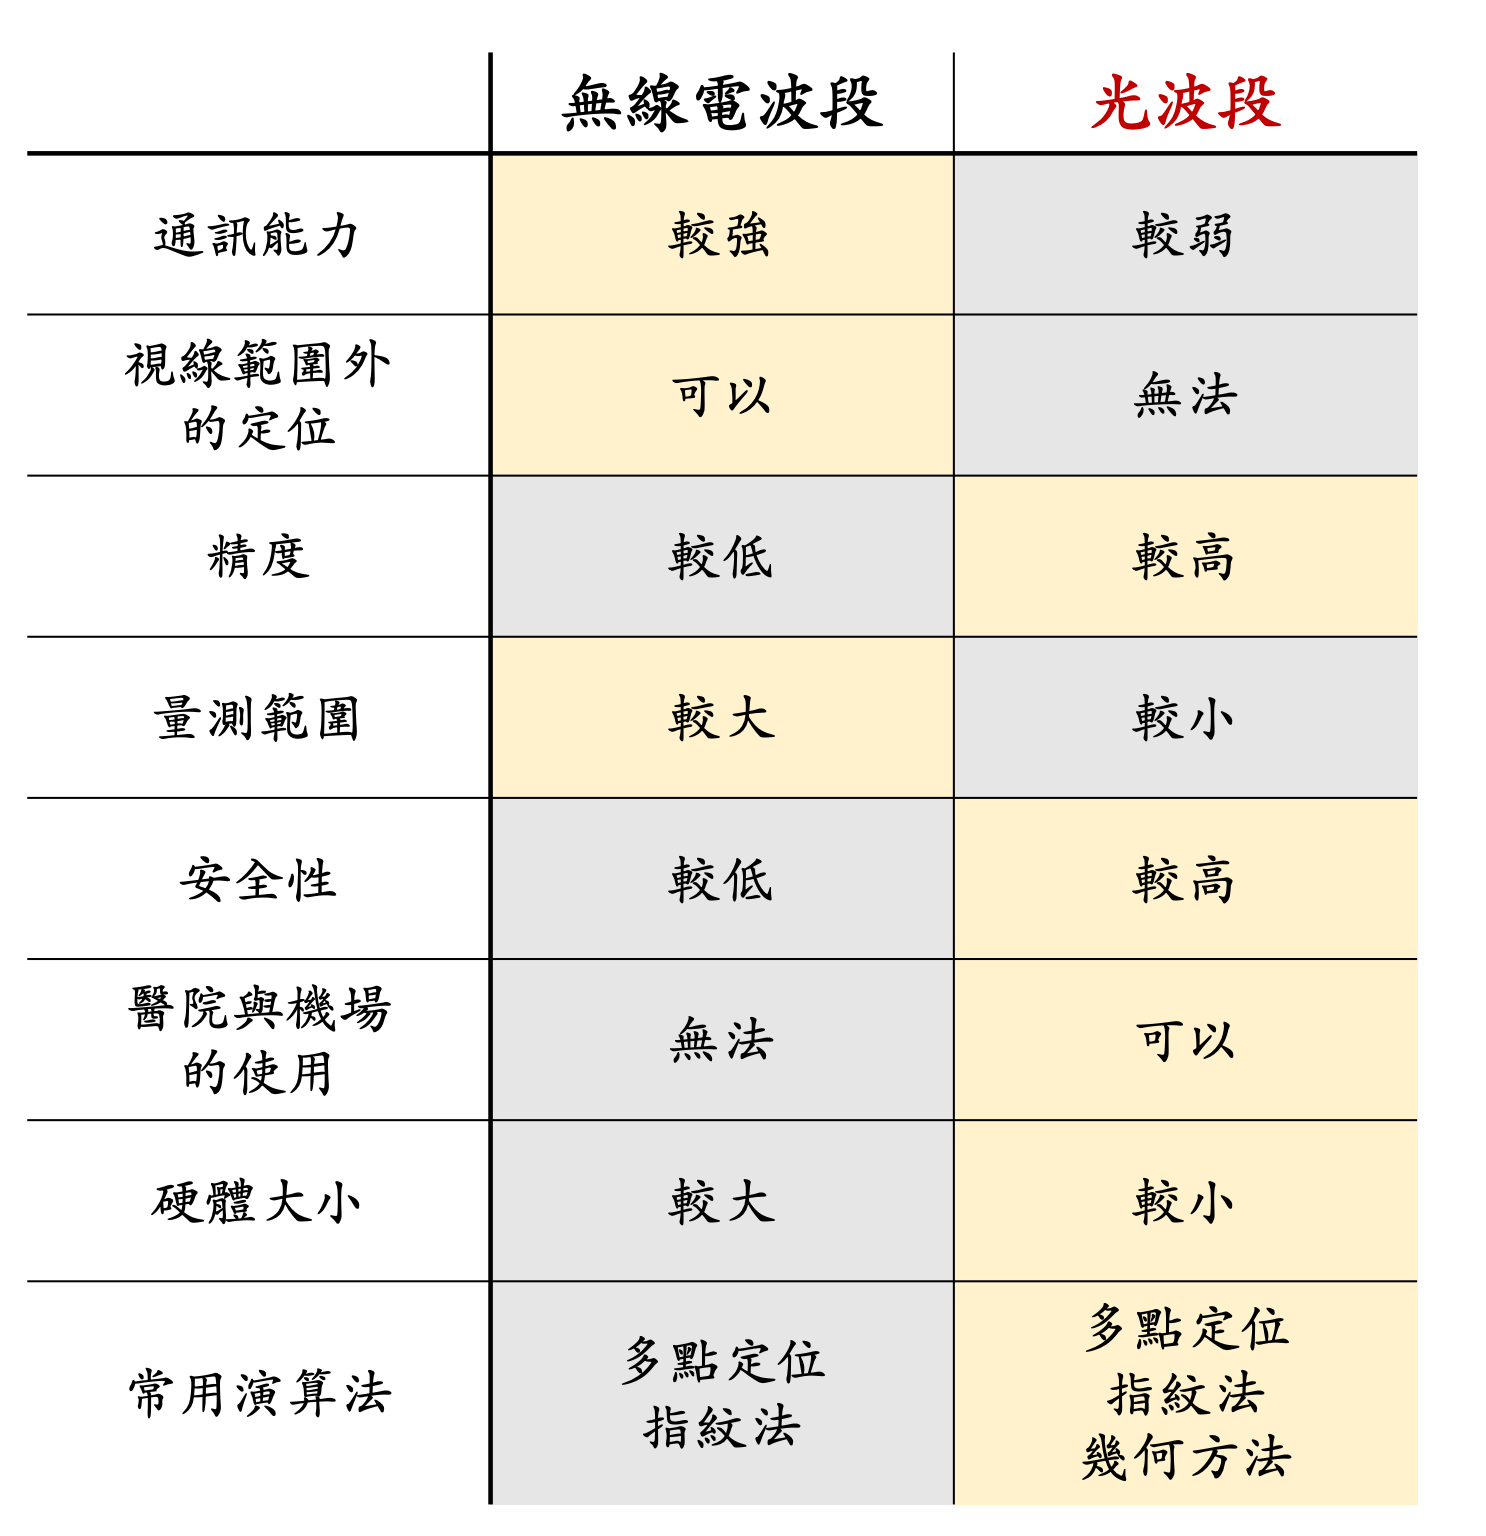
\includegraphics[width=11cm]{ch2pic/method_compare.png}   
            \end{table}


            光波段定位也可以依照使用波段與使用感測氣分類如圖\ref{pic:electro_sort},以下分別於\ref{chp:light_electro}章探討使用波段的差異,以及於\ref{chp:light_receiver}章介紹感測器硬體技術的選擇。


            \subsubsection{依照波段分類:紅外光、近紅外光與可見光}

            \label{chp:light_electro}

            如圖\ref{pic:electro_sort},光波段依照人眼可視與否分成可見光與紅外光兩類,而其中紅外光內由於硬體特性不同,又分為近紅外光與遠紅外光。以下依照不同面向條列討論:

            \begin{description}

                \item[- 人眼可視與否]\hfill 
                
                \qquad
                依照人眼可視區分為可見光與紅外光波段,而紅外光頻率低、能量較小,且於視網膜成像的難度也大,因此較為安全。而可見光的優勢於其可以照明,因此大多可見光定位會應用於需照明的場域,配合照明用的光線進行定位。但凡使用情境不想影響人們的感知,亦或是光源需移動,有直射眼境造成人眼不適的可能時,便會選擇使用紅外光波段。

                \qquad 
                本研究目標需應用於移動物體上,因此紅外光呈現優勢,紅外光無法在視網膜成像的特性讓使用者並不會感受到不適

                \item[- 成本] \hfill 
                
                \qquad
                光波段的光感測器常見的材料有矽(Si)、鍺(Ge)與III或V族元素,價格最便宜的是矽材料,而矽感測器的感光波段約在400-1000nm,也就是可見光與近紅外光(NIR)波段。若要量測波長較長的紅外光,硬體材料便需要使用到昂貴的鍺或其他三五族元素\cite{si_pd},這也是為什麼普遍紅外光波段的硬體的印象都較為昂貴。實際上,近紅外光波段的感測器可挑選與可見光感測器相同的矽材料,使成本維持低。

                \qquad
                除了硬體本身的成本以外,系統架設難易度也需納入考量。常見可見光定位的文獻會強調系統架設難易度低,因為可見光定位可以利用室內現有的照明光源,不需額外添置訊號發射器\cite{vlc_adv}。然而需注意的是,當可見光定位需利用光通訊分辨ID時,使用者需要在光源硬體加裝驅動器,且原有燈具需改成符合編碼需求的硬體,所需付出的成本不得被忽視。因此,在架設成本上,我認為波段的無論影響不大。
                
                \qquad
                因此,僅考量成本時,無論是PD還是影像感測器,挑選可見光與近紅外光波段較為合適。
        
                \item[- 環境光源的影響] \hfill 
                
                \qquad
                光波段的誤差來源主要包含多重路徑傳輸(Multipath effect)與環境光源(Ambious Light Source)\cite{survey_light2020},其中多路徑傳輸無關波段,影響程度皆相同。而環境光源的部分,強度過高可造成訊號偏移,甚至硬體飽和導致訊號失真,因此需有效的降低環境光源的強度以保持定位的準確度。
            
                

                \qquad
                環境光源包含了室內的光源以及太陽光源,室內的光源使用交流電的頻率約在120hz,可以針對頻率進行濾波。而太陽光源的強度與電磁波頻率有關,關係呈現於太陽輻射波譜(Solar Irradiance Spectrum)如圖\ref{pic:solar_spectrum},其顯示太陽光強度與波長的關係。其中,太陽光照射至地球並傳送至地表的能量與大氣層的吸收度有關,因此輻射波譜圖的高峰即為可見光波段,光波段中有幾個低谷,出現在760nm左右的氧氣吸收帶(Oxygen A-band)、與940nm和1550nm附近被水蒸氣吸收之波段\cite{book:solar_spectrum}。
                
                \begin{figure}[htpb]
                    \centering
                    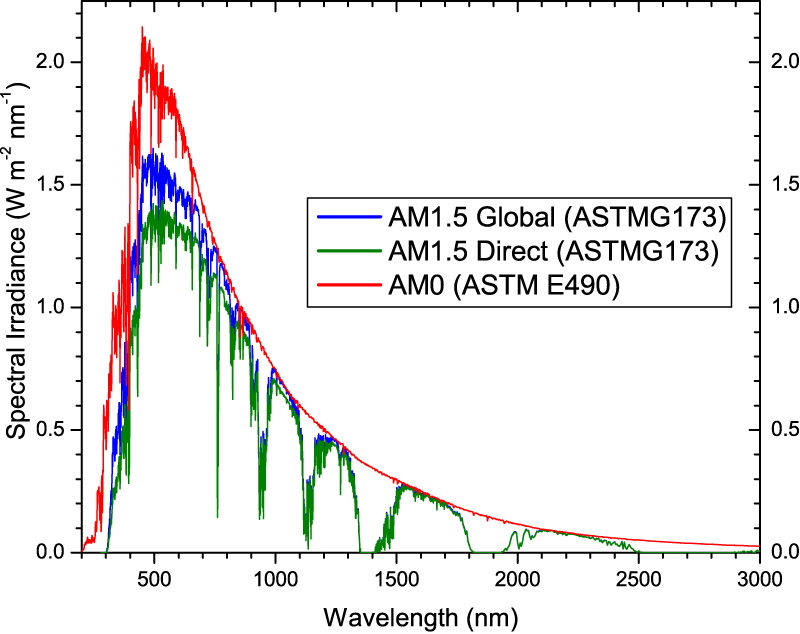
\includegraphics[width=10cm]{ch2pic/solar_spectra.png}
                    \caption{太陽輻射波譜\cite{astm}}
                    \label{pic:solar_spectrum}
                \end{figure}

                \qquad
                由於利用光波段定位最大誤差來源之一就是要克服其他光所造成的雜訊,因此在選擇工作波長時,需挑選太陽光能量較低的波段,例如於近紅外光波段中的760nm與940nm,以及遠紅外光波段內的1550nm。
        
                \end{description}
                


                \hfill
                綜上所述,根據本研究的需求,將各波段的優缺點簡單整理於表\ref{pic:light_freq_compare},最適合本研究需求的波段為近紅外光波段中的太陽能量低谷區。利用這些波段進行定位,可以同時節省硬體成本、降低環境光源的影響,也能夠不造成使用者的眼經不適。

                \begin{table}[htpb]
                    \caption{光波段中的波段特性比較}
                    \label{pic:light_freq_compare}
                    \centering
                    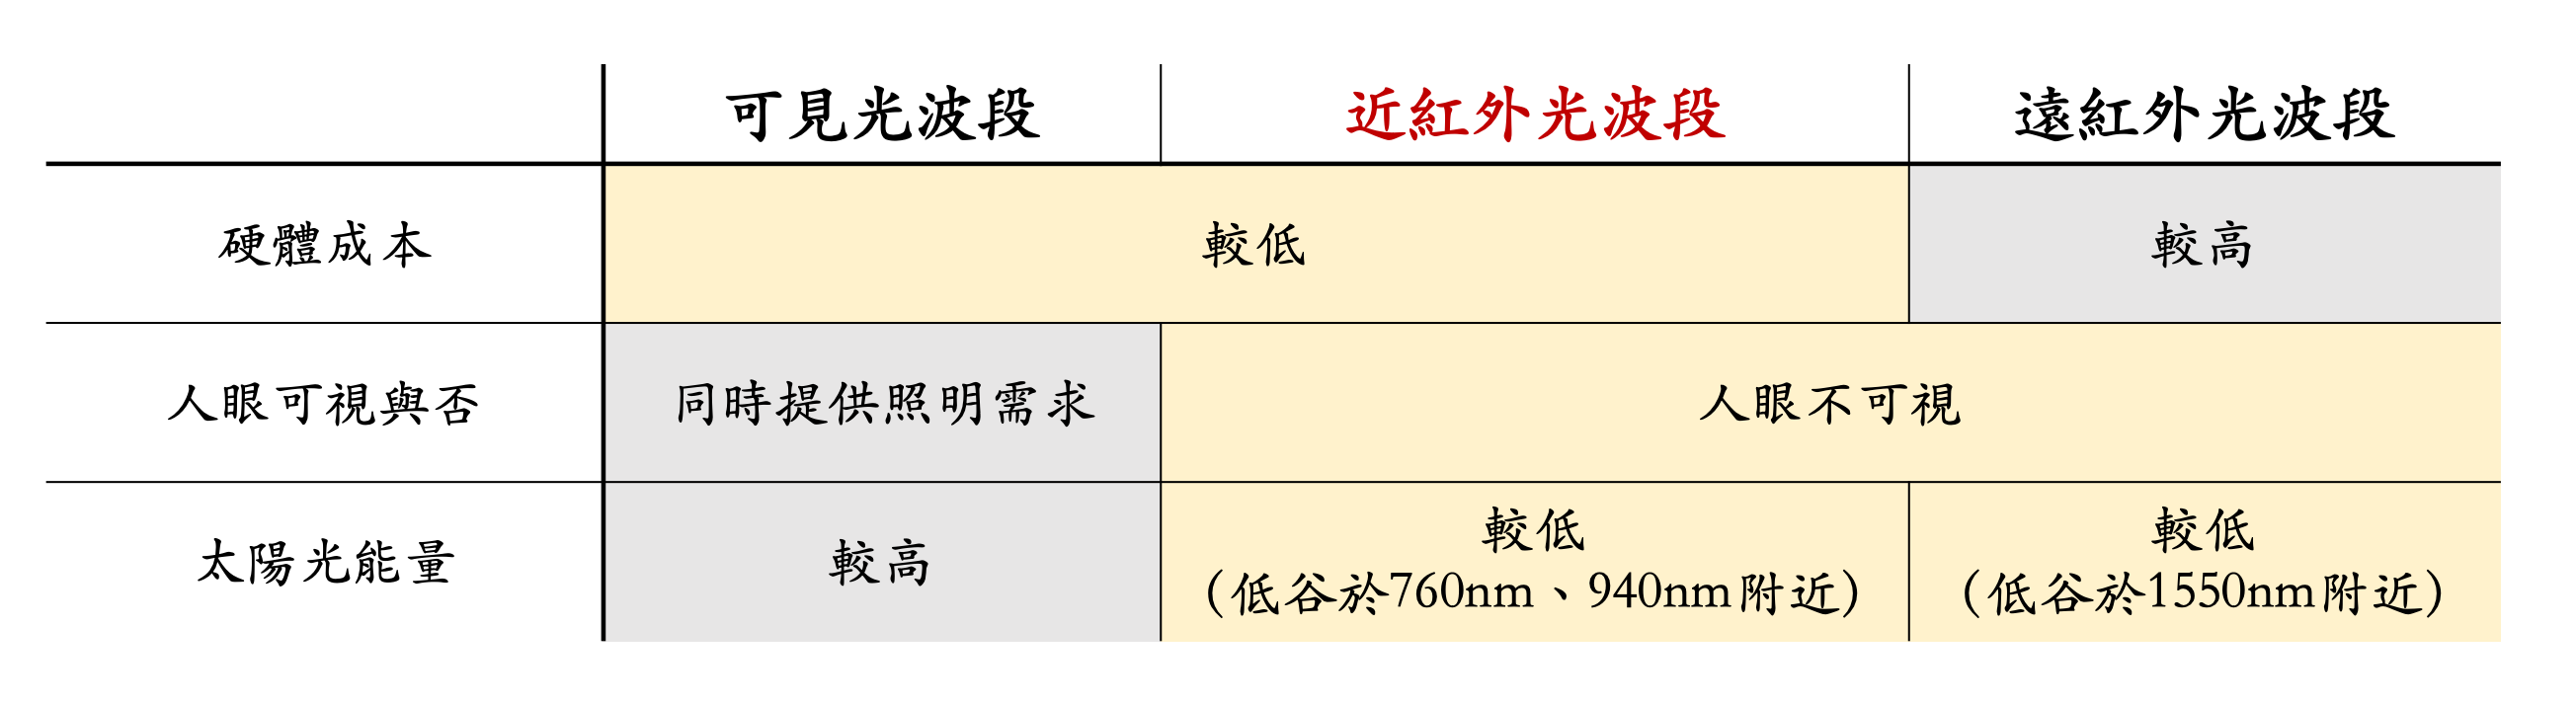
\includegraphics[width=16cm]{ch2pic/light_freq_compare.png}
                \end{table}


            \subsubsection{依接收子類型分類:PD與影像感測器}
            \label{chp:light_receiver}

                

                \ref{chp:light_electro}章中討論了光波段中不同波段的優缺點,而本小節中將討論光波段中常使用的兩種硬體差別,其分別為PD與影像感測器。

                \begin{description}

                    \item[- 影像感測器]\hfill 
                    
                    \qquad
                    影像感測器包含常見的相機,運作原理為每次取樣時,影像感測器擷取多個像素的光強度資訊,資訊量極多,是眾多定位技術中最消耗運算資源以及硬體成本最高的。其Step4.的定位演算法方是利用辨識已知的特徵圖案,進而將影像中特徵圖案的大小、變形量與特徵圖案的尺寸、形狀進行比對,利用PnP演算法推算目標物的距離以及姿態(如\ref{chp:method-algorithm}章)。其中,投射於影像平面上的圖案大小隨距離增加,以平方衰減,因此特徵圖案需要越大越好。除此之外,影像感測器的取樣頻率大多在百赫茲內,且視覺辨識所需要的運算資源多,因此成本高,且運算速度也較慢。

                    \qquad
                    影像感測器所辨識的特徵點又可分為主動與被動傳送訊號,被動傳送訊號的包含ArUco標誌(圖\ref{pic:aruco}),其需透過環境光源照射可見光波並反射至影像感測器,讓影像感測器得以看到標誌;若室內光源未開,則無法定位。反之,主動傳送訊號的標誌便是光源,大多室內定位會使用半徑15公分以上的崁燈,利用影像感測器的滾動式快門效應(Rolling Shutter Effect),將條紋圖案視為特徵辨識。其中,滾動式快門效應會造成條紋圖樣的原因如圖\ref{pic:rolling_shutter},因為CMOS感測器並非同時進行所有像素的成像,而是輪流一列一列的成像,搭配光源的閃爍,各列成像時便會各自呈現亮或暗的樣式進而產生條紋樣式。除此之外,透過調整光源的閃爍頻率,使用者可以調整條紋的粗細,進而達到編碼與解碼的效果,如圖\ref{pic:rolling_shutter_case}。

                    \begin{figure}[htpb]
                        \centering
                        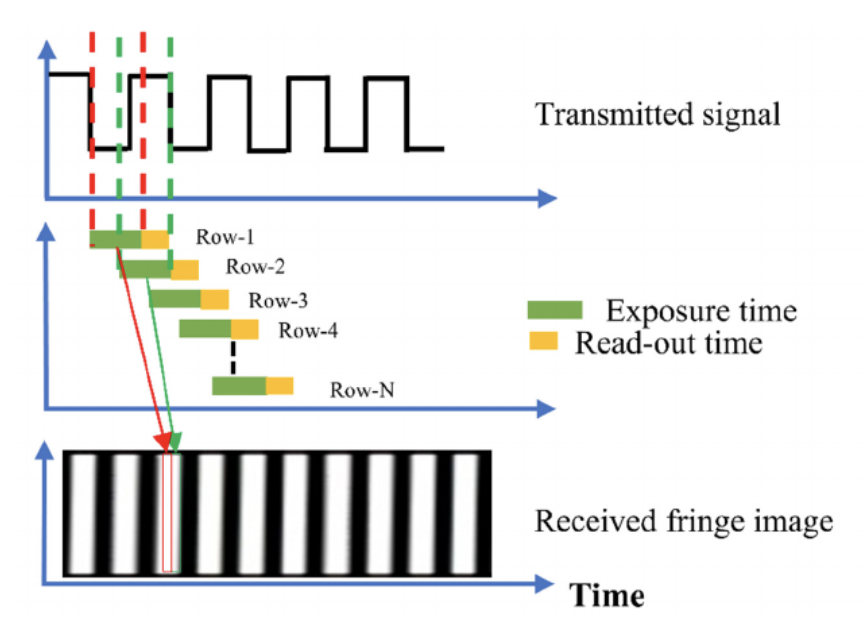
\includegraphics[width=12cm]{ch2pic/rolling_shutter.png}
                        \caption{滾動式快門效應的成因\cite{pic:rolling_shutter}}
                        \label{pic:rolling_shutter}
                    \end{figure}

                    \begin{figure}[htpb]
                        \centering
                        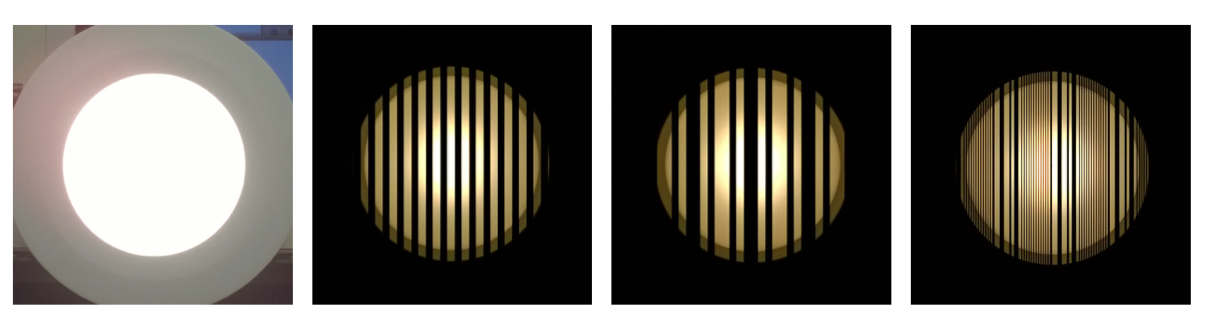
\includegraphics[width=10cm]{ch2pic/rolling_shutter_case.png}
                        \caption{滾動式快門效應產生的條紋樣式\cite{pic:rolling_shutter_case}}
                        \label{pic:rolling_shutter_case}
                    \end{figure}

                    \qquad
                    光波段中除了環境光源會造成誤差以外,誤差主要來源為多重路徑傳輸,如圖\ref{pic:multipath}所示,有部分訊號傳送至障礙物後遭反射傳入感測氣中,使得感測器接收的訊號除了LoS路徑以外,還包含了透過反射傳送而來的訊號,這些感測器量測到的NLoS訊號便會造成誤差。而影像感測器使用的為影像中的特徵點,因此較不受多重路徑傳輸的影響,在此項誤差上具有優勢。

                    \begin{figure}[htpb]
                        \centering
                        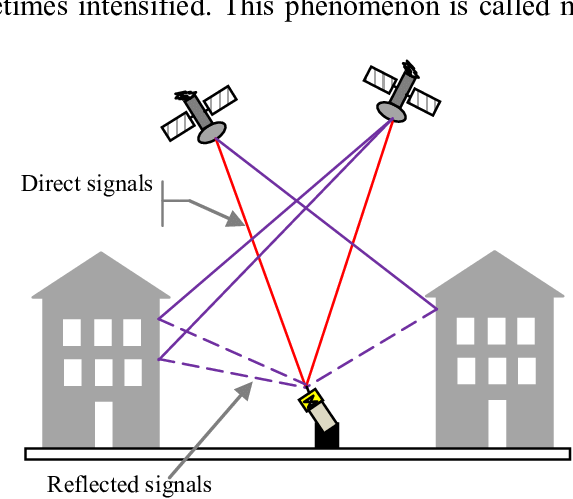
\includegraphics[width=8cm]{ch2pic/multipath.png}
                        \caption{多重路徑傳輸\cite{pic:multipath}}
                        \label{pic:multipath}
                    \end{figure}

                    \item[- Photodiode(PD)]\hfill
                    
                    \qquad
                    光電二極體(Photodiode,以下簡稱PD)能感測到資訊僅有強度資訊,而強度資訊受LED出射角度、PD入射角度、距離影響(於\ref{chp:LEDPD_hardware}章詳述),相較大多無線電波技術的訊號強度主要僅受距離影響,PD的變數較多,使得獲得相對定位的演算法也較複雜,需要多個PD或多個LED以進行定位。然而PD優勢為具有極高的取樣頻率,可高達千赫茲甚至萬赫茲,高取樣頻率即可使用光通訊進行編碼與解碼,且硬體成本相較影像感測器來說非常低。

                    \qquad
                    LED與PD定位的次系統常有多個硬體一同組成,而由於光強度同時與出入射角度和距離相關,因此Step1.次系統設置時可將多個硬體以不同姿態或位置擺設來進行定位的計算。以研究\cite{case:ml}為例的PD次系統設計如圖\ref{pic:ml_pd_config},其便將多個PD以不同指向擺放固定。

                    \begin{figure}[htpb]
                        \centering
                        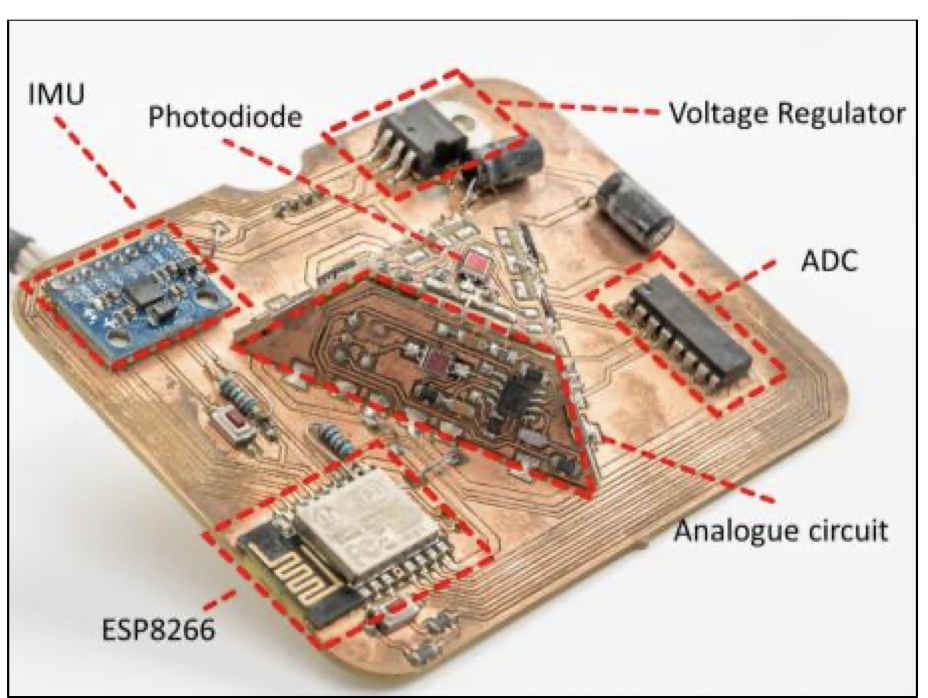
\includegraphics[width=10cm]{ch2pic/ml_pd_config.png}
                        \caption{文獻提供之PD次系統設計\cite{case:ml}}
                        \label{pic:ml_pd_config}
                    \end{figure}

                    \qquad
                    Step3.PD量測訊號的流程如圖\ref{pic:vlc_flow}所示,訊號發送是利用驅動器與LED進行光通訊訊號發送,PD接收訊號後進行解碼、取得LED的ID與光強度,再利用光強度以不同演算法解出相對位置。而LED與PD的定位系統中,硬體組成可以為單LED對多PD、多LED對多PD、或是多LED對多PD,其中,當系統內包含多個LED時,各PD會同時接收到來自多個LED,而多個LED訊號的解碼如圖\ref{pic:vlc_multi_pd},PD會將訊號轉換至頻域,以獲得各頻率下的強度,也就是各LED傳送至各PD的強度。

    
                    
                    \begin{figure}[htpb]
                        \centering
                        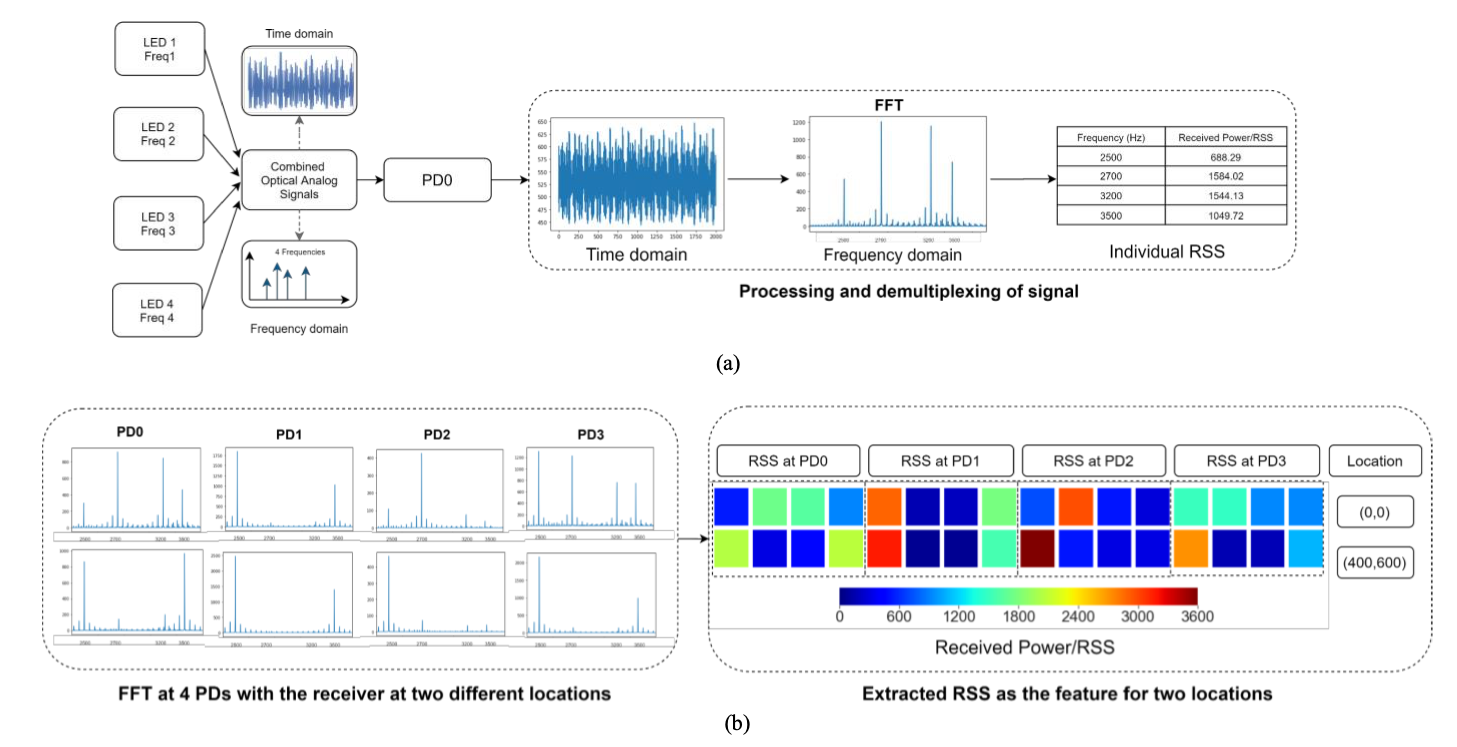
\includegraphics[width=15cm]{ch2pic/vlc_multi_pd.png}
                        \caption{多PD進行光通訊解碼\cite{case:ml}}
                        \label{pic:vlc_multi_pd}
                    \end{figure}

                    \qquad
                    利用光通訊獲得各LED傳送至各PD的強度後,Step4.解出定位的演算法分成兩類,一類型為使用指紋法或多點定位,這種類型的系統需在環境中放置多個參考點(如圖\ref{pic:env_finger}),為「環境對一點的定位」。除此之外,大多使用\ref{chp:method-algorithm}章中提到的幾何方法,如\cite{case:3d_layers}(如圖\ref{pic:env_1to1}),透過多PD量測強度後,利用多個PD強度與幾何之間的關係取得定位,方法詳述於\ref{chp:LEDPD_now}章中。

                    \begin{figure}[htpb]
                        \centering
                        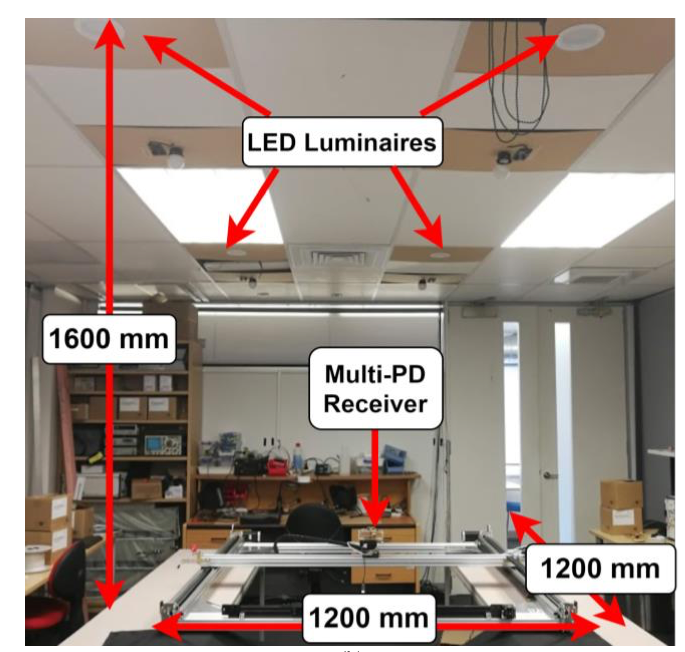
\includegraphics[width=8cm]{ch2pic/env_finger.png}
                        \caption{文獻\cite{case:ml}的系統架構(使用指紋法)}
                        \label{pic:env_finger}
                    \end{figure}

                    \begin{figure}[htpb]
                        \centering
                        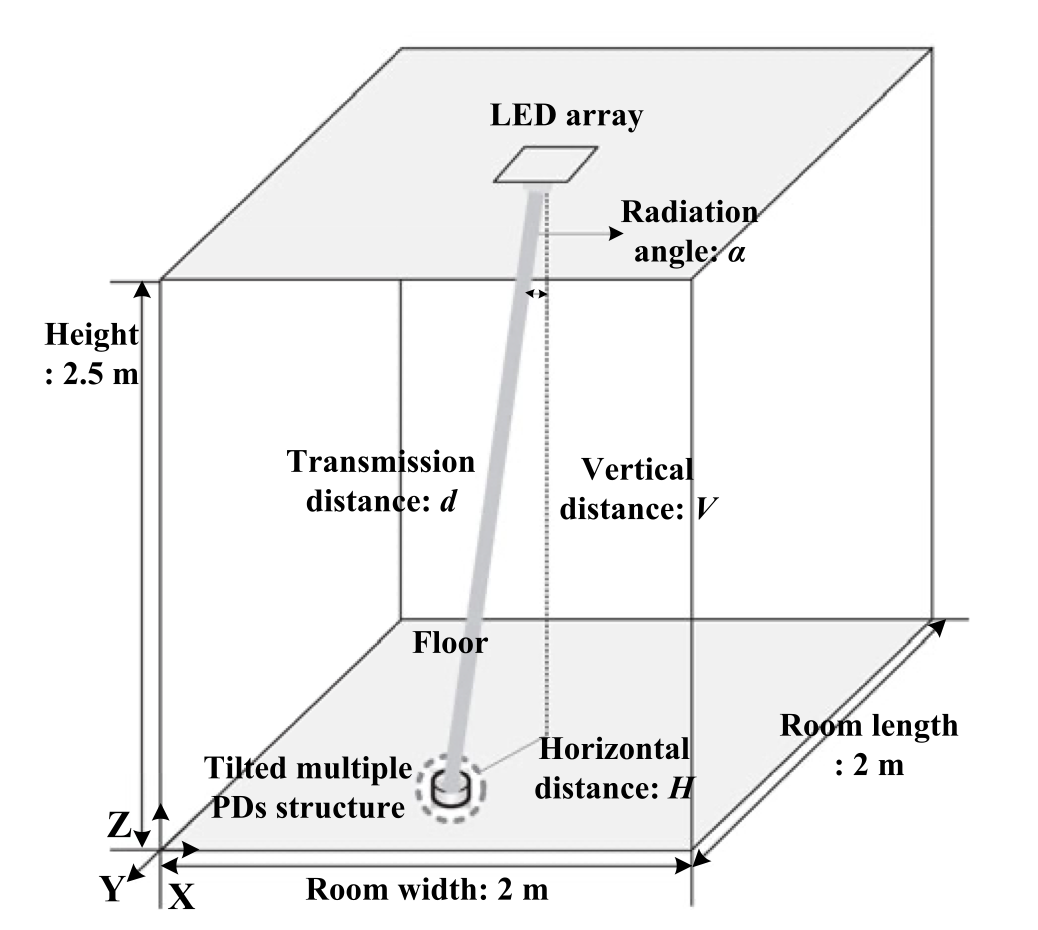
\includegraphics[width=10cm]{ch2pic/env_1to1.png}
                        \caption{文獻\cite{case:3d_layers}的系統架構(使用幾何方法)}
                        \label{pic:env_1to1}
                    \end{figure}

                \end{description}

                \hfill
                影像感測器與PD進行定位的方法差異非常大,前者演算法為影像辨識,利用特殊圖案分辨光源,以影像中的變形計算位置;PD常見的定位演算法則包含多點定位、指紋法、幾何方法,利用光通訊分辨光源。在兩者之間權衡時,本研究主要考量到成本以及硬體大小,為了能夠達到靈活、廣泛運用,取捨掉影像感測器具有高精度可能性的優勢。


                \begin{table}[htpb]
                    \centering
                    \caption{影像感測器與PD的特性比較}
                    \label{pic:pd_camera_sort}
                    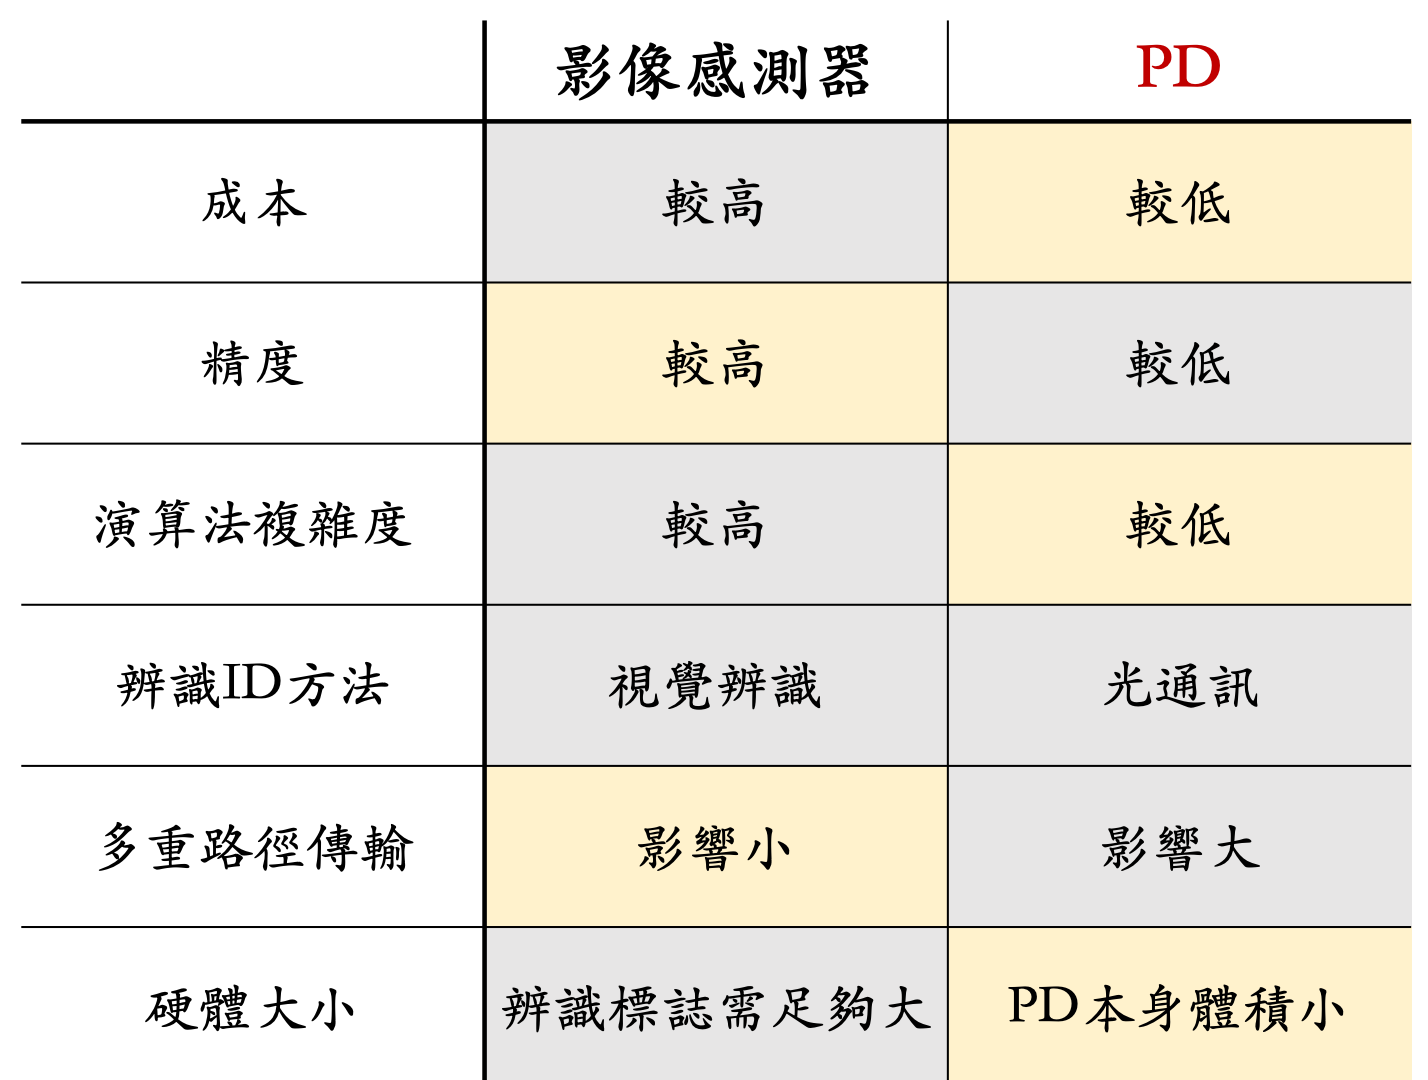
\includegraphics[width=10cm]{ch2pic/pd_camera_sort.png}     
                \end{table}

                


        
                

        \subsection{小結:本研究使用技術的選擇}
        

        在\ref{chp:technique}章中,由電磁波頻率分類為無線電波段與光波段,分別於\ref{chp:radio}章與\ref{chp:light}章中介紹無線電波與光波段的定位,並於圖\ref{pic:method_compare}中比較兩者,其中光波段較高的精度、較小的硬體、以及能夠靈活應用的幾何方法演算法,使光波段定位為更適合的選擇。

        光波段中,又依照使用波段與使用的硬體分類。使用波段於\ref{chp:light_electro}章中討論,分為可見光、近紅外光與遠紅外光,如表\ref{pic:light_freq_compare},近紅外光兼具低成本低干擾的特色,因此選用近紅外光波段中,位於輻射光譜低谷的760nm與940nm波段最為合適。硬體選擇則於\ref{chp:light_receiver}章中討論,如表\ref{pic:pd_camera_sort},權衡之下選擇PD,雖然捨棄精度,但得以換取較低的成本與較小的體積;另外,PD所使用的定位演算法需為具有單點對單點定位能力的幾何方法。
    
        
        綜上所述,本論文將使用LED與PD的定位方法,於後續的\ref{chp:LEDandPD}章中更深入的討論,分別介紹LED與PD的特性、光傳遞模型,以及現今文獻所遇困難與限制。


        

    

        

        

        

        


        

        

            

          
\section{LED與PD的定位系統}
\label{chp:LEDandPD}




\begin{figure}[htpb]
    \centering
    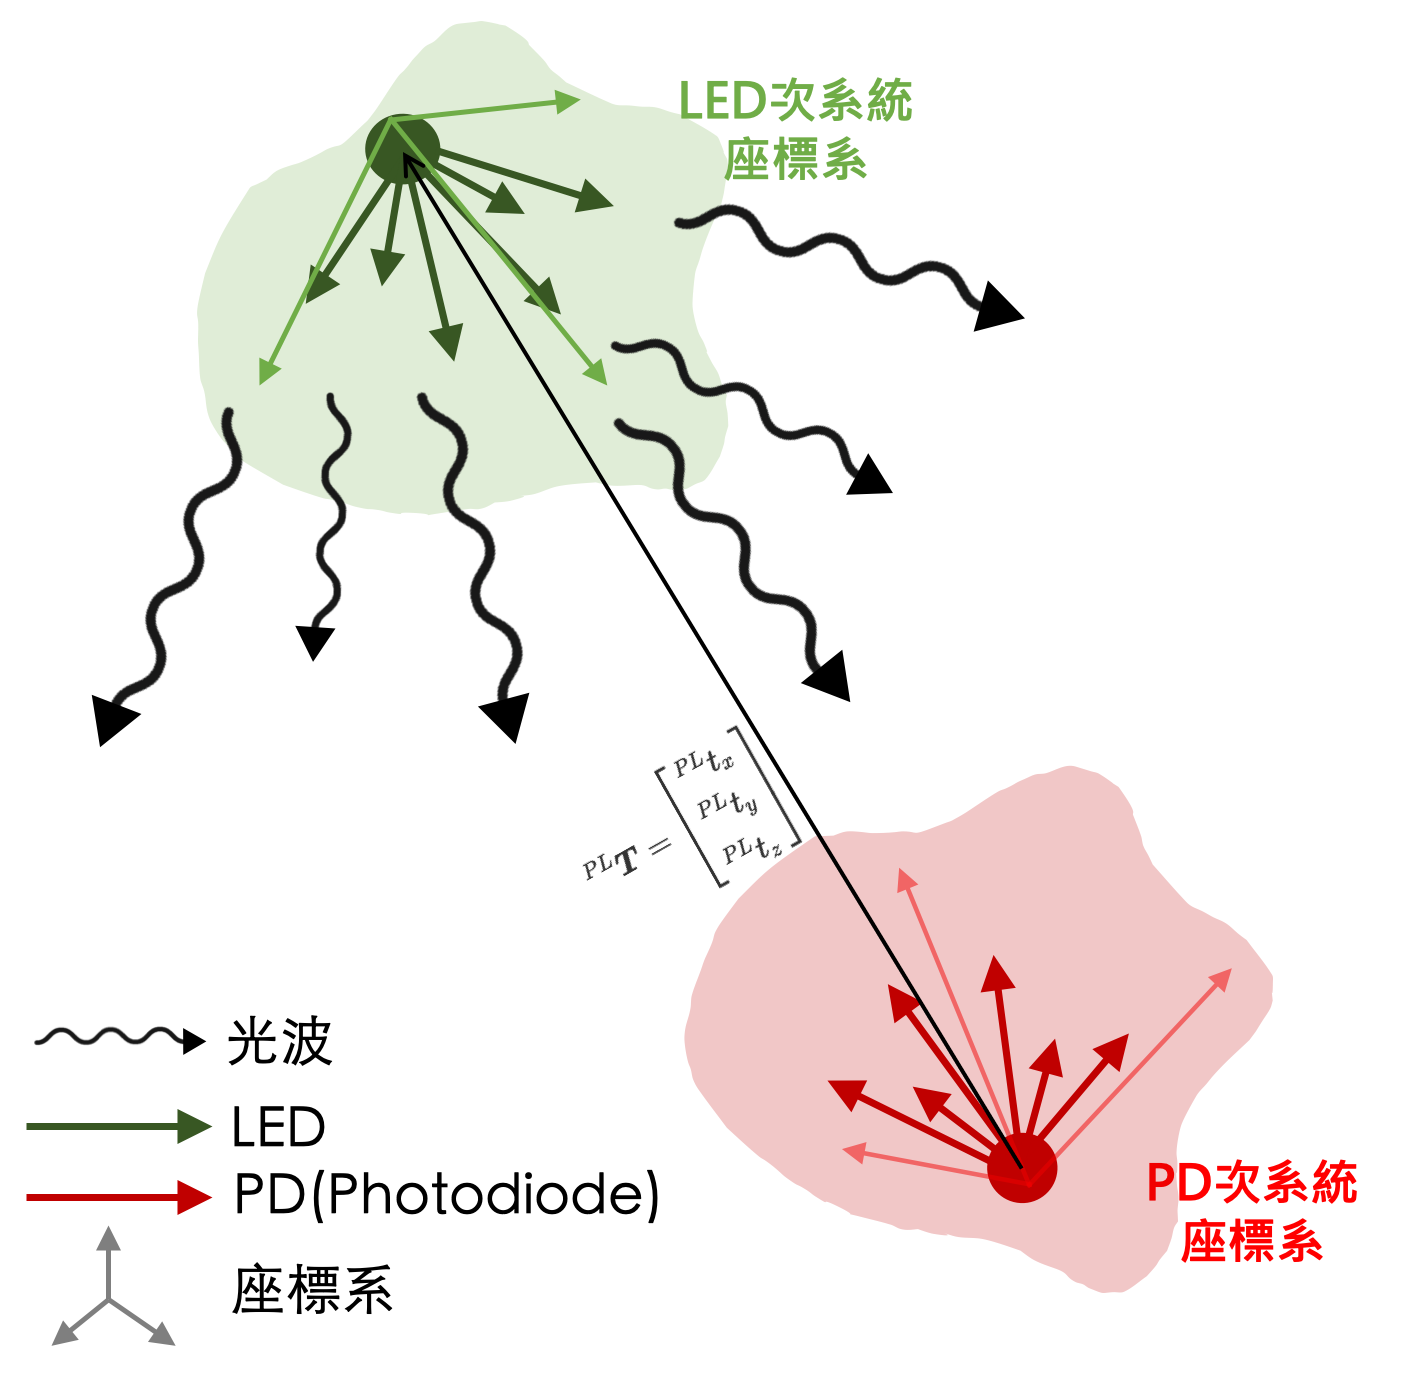
\includegraphics[width=11cm]{ch2pic/lp_system_structure.png}
    \caption{LED與PD定位系統架構}
    \label{pic:lp_system_structure}
\end{figure}




LED與PD的定位系統架構如圖\ref{pic:lp_system_structure},是由$L$個LED與$P$個PD組成,在文獻中,$L$與$P$的數量可為一也可為多個。根據\ref{chp:motivate}章中提到的使用情境,我們希望將LED與PD各自封裝成兩硬體單位,因此可用兩座標系表示兩硬體單位。其中,多個LED固定於LED座標系上,PD則是固定在PD座標系上,而兩座標系的相對關係可以自由的改變如\ref{chp:relative}章所述。實體的系統架構如圖\ref{pic:env_finger},其為\cite{case:ml}中的系統架構,而圖\ref{pic:ml_pd_config}則為該研究中的PD量測單位。

\begin{figure}[htpb]
    \centering
    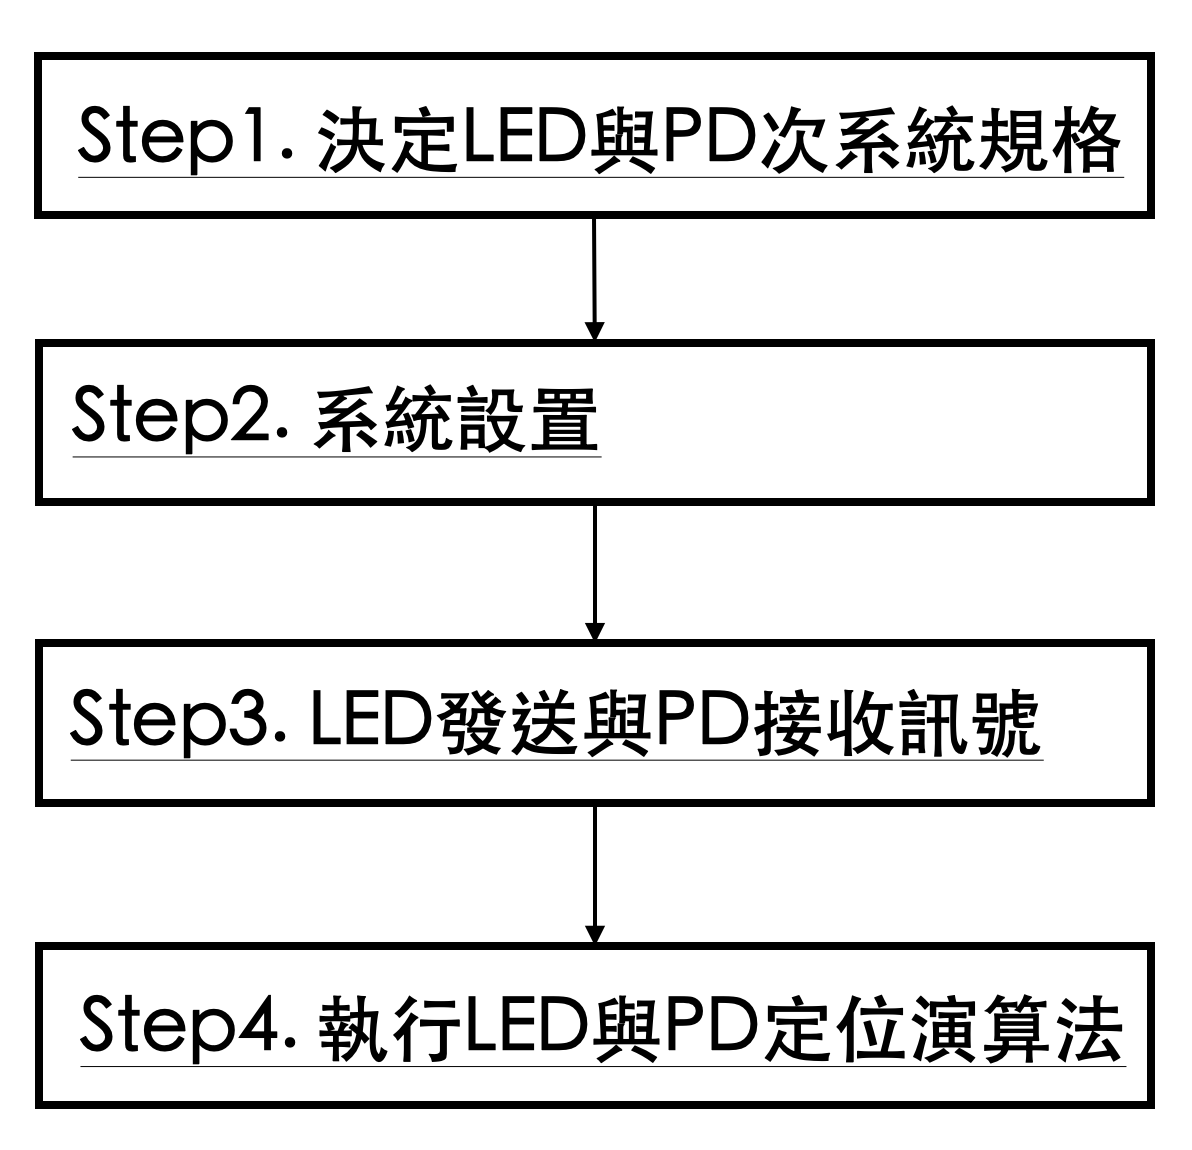
\includegraphics[width=7cm]{ch2pic/lp_system_flow.png}
    \caption{LED與PD定位系統流程}
    \label{pic:lp_system_flow}
\end{figure}

LED與PD系統的定位流程則如圖\ref{pic:lp_system_flow},步驟與圖\ref{pic:pos_flow}中的步驟相同,僅是針對LED與PD系統進行微調,以下分項介紹:
    

\begin{description}
    \item[Step1. 決定LED與PD次系統規格:]
    
    \hfill
    
        \begin{itemize}
            \item 決定使用的LED與PD硬體規格(詳述於\ref{chp:lambertian}章與\ref{chp:LEDPD_hardware}章)
            \item 將LED硬體與驅動器等電路連接
            \item PD需與放大器或是電阻連接完成感測電路  
            \item 設置兩次系統中硬體擺設的方式(詳述於\ref{chp:config}章)
        \end{itemize}

    \item[Step2. 系統設置:] 
    
    \hfill
    
    \qquad 
    完成兩次系統的前置作業後,進行Step2.系統設置,也就是將兩次系統擺設於空間中欲量測的位置,呈現如圖\ref{pic:lp_system_structure}中呈現的系統架構,兩座標系之間的轉換如\ref{chp:relative}章中的齊次座標轉換矩陣。

    \item[Step3. LED發送與PD接收訊號]\hfill
    
    \begin{figure}[htpb]
        \centering
        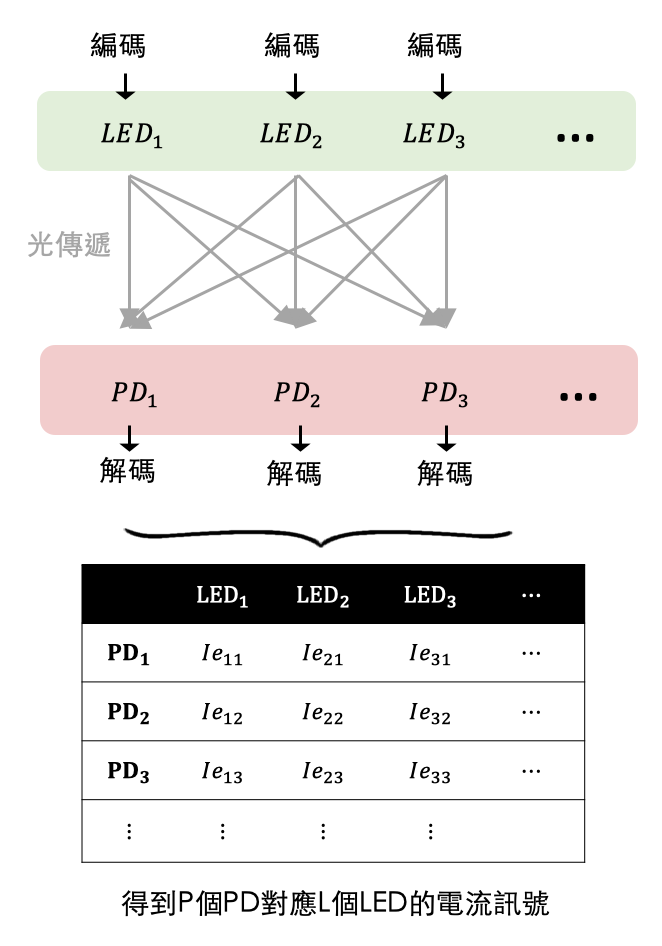
\includegraphics[width=10cm]{ch2pic/vlc_flow_draw.png}
        \caption{Step3.中的光通訊流程圖}
        \label{pic:vlc_flow_draw}
    \end{figure}

    \qquad
    為了能夠辨識是哪個LED發出的訊號,系統需要透過光通訊技術進行邊解碼。光通訊流程圖如圖\ref{pic:vlc_flow_draw},由LED編碼傳輸特定模式的訊號,而在光定位上最常使用的編碼方式為OOK,其僅利用開關頻率將LED的ID傳輸。LED發出的光訊號透過光傳遞至PD,每個PD將所收到的訊號進行光通訊解碼,將訊號拆成訊號來自哪個LED以及該LED所造成的電流大小,綜合$P$個PD解碼後的資訊,即可獲得一$L\times P$的表格,顯示各PD對應各LED的電流強度,而理論上的電流強度可以用光傳遞模型描述,詳述於\ref{chp:model}章中。
    
    \item[Step4. 執行LED與PD定位演算法] \hfill
    
    \qquad
    執行定位演算法則是透過Step3.所獲得的$L\times P$各PD對應各LED的電流表格,回推出兩座標系的相對位置,如同\ref{chp:method-algorithm}章敘述,PD能使用的定位演算法種類包含多點定位、三角法、指紋法與幾何類型,前三種都為多點對一目標物的定位,系統環境與架構如圖\ref{pic:env_finger},並不符合本研究目標欲達到的兩單位之間的互相定位,如圖\ref{pic:env_1to1};因此,以下針對幾何類型介紹。

    \qquad
    使用幾何方法的演算法,主要是仰賴光傳播模型中(式\ref{eqn:model}),PD的電流與距離、出入射角相關,利用多個LED與PD之間的交互關係,得到相對位置。光傳遞模型中,變數除了距離以外,還包含出入射角,使得PD具有獲得但點對單點定位的能力,例如PD得以透過特殊的限制與組態,得到目標物的姿態\cite{case:orient},是除了影像感測器以外能得到姿態資訊的方法。然而也因為變數較多,使得模型較為複雜,如同式\ref{eqn:model_coor_extend}呈現,因此需透過適當的限制簡化模型複雜度,常見的限制於\ref{chp:LEDPD_restrict}章中介紹。


\end{description}

\onehalfspacing

為深入了解LED與PD定位系統,我們先於\ref{chp:LEDPD_theorum}中介紹LED與PD的定位理論,再於\ref{chp:LEDPD_now}章中介紹現今LED與PD定位方法與應用,以及\ref{chp:LEDPD_problem}章中整理現今所遇困難。


\subsection{LED與PD的定位理論}  
\label{chp:LEDPD_theorum}

    在進入LED與PD定位系統的現況前,我們需先對LED與PD定位系統的原理有所了解。本章節依續從\ref{chp:light_unit}章光領域常用的單位介紹開始,有了基本理解後則進入\ref{chp:lambertian}章介紹朗博次方模型與\ref{chp:LEDPD_hardware}章中的LED與PD硬體特性,最後則於\ref{chp:model}章介紹光傳遞模型。

    \subsubsection{光領域常用單位介紹}
    \label{chp:light_unit}
    
    由於光領域中,單位與術語經常有口語或混用的情況,令人感到困惑,因此在進入PD與LED定位的探討之前,先對光領域的一些術語與單位進行介紹,方便\ref{chp:lambertian}章以及\ref{chp:model}章中敘述朗博輻射模型與光傳播模型。

    首先,描述光照的單位分為兩種系統:輻射測量學(Radiometry)與光度測量學(Photometry),兩領域以不同單位描述光源如表\ref{tab:photometry},其中輻射測量學著重在電磁波輻射的量測,描述通量單位為瓦特(Watt);而光度測量學著重在人眼可見之可見光波段的研究,通量單位為流明(Lumen),同樣物理量下單位定義不同\cite{radiometry_and_photometry}。
    

    \begin{table}[htpb]
        \centering
        \caption{輻射測量學與光度測量學的物理量比較}
        \label{tab:photometry}
        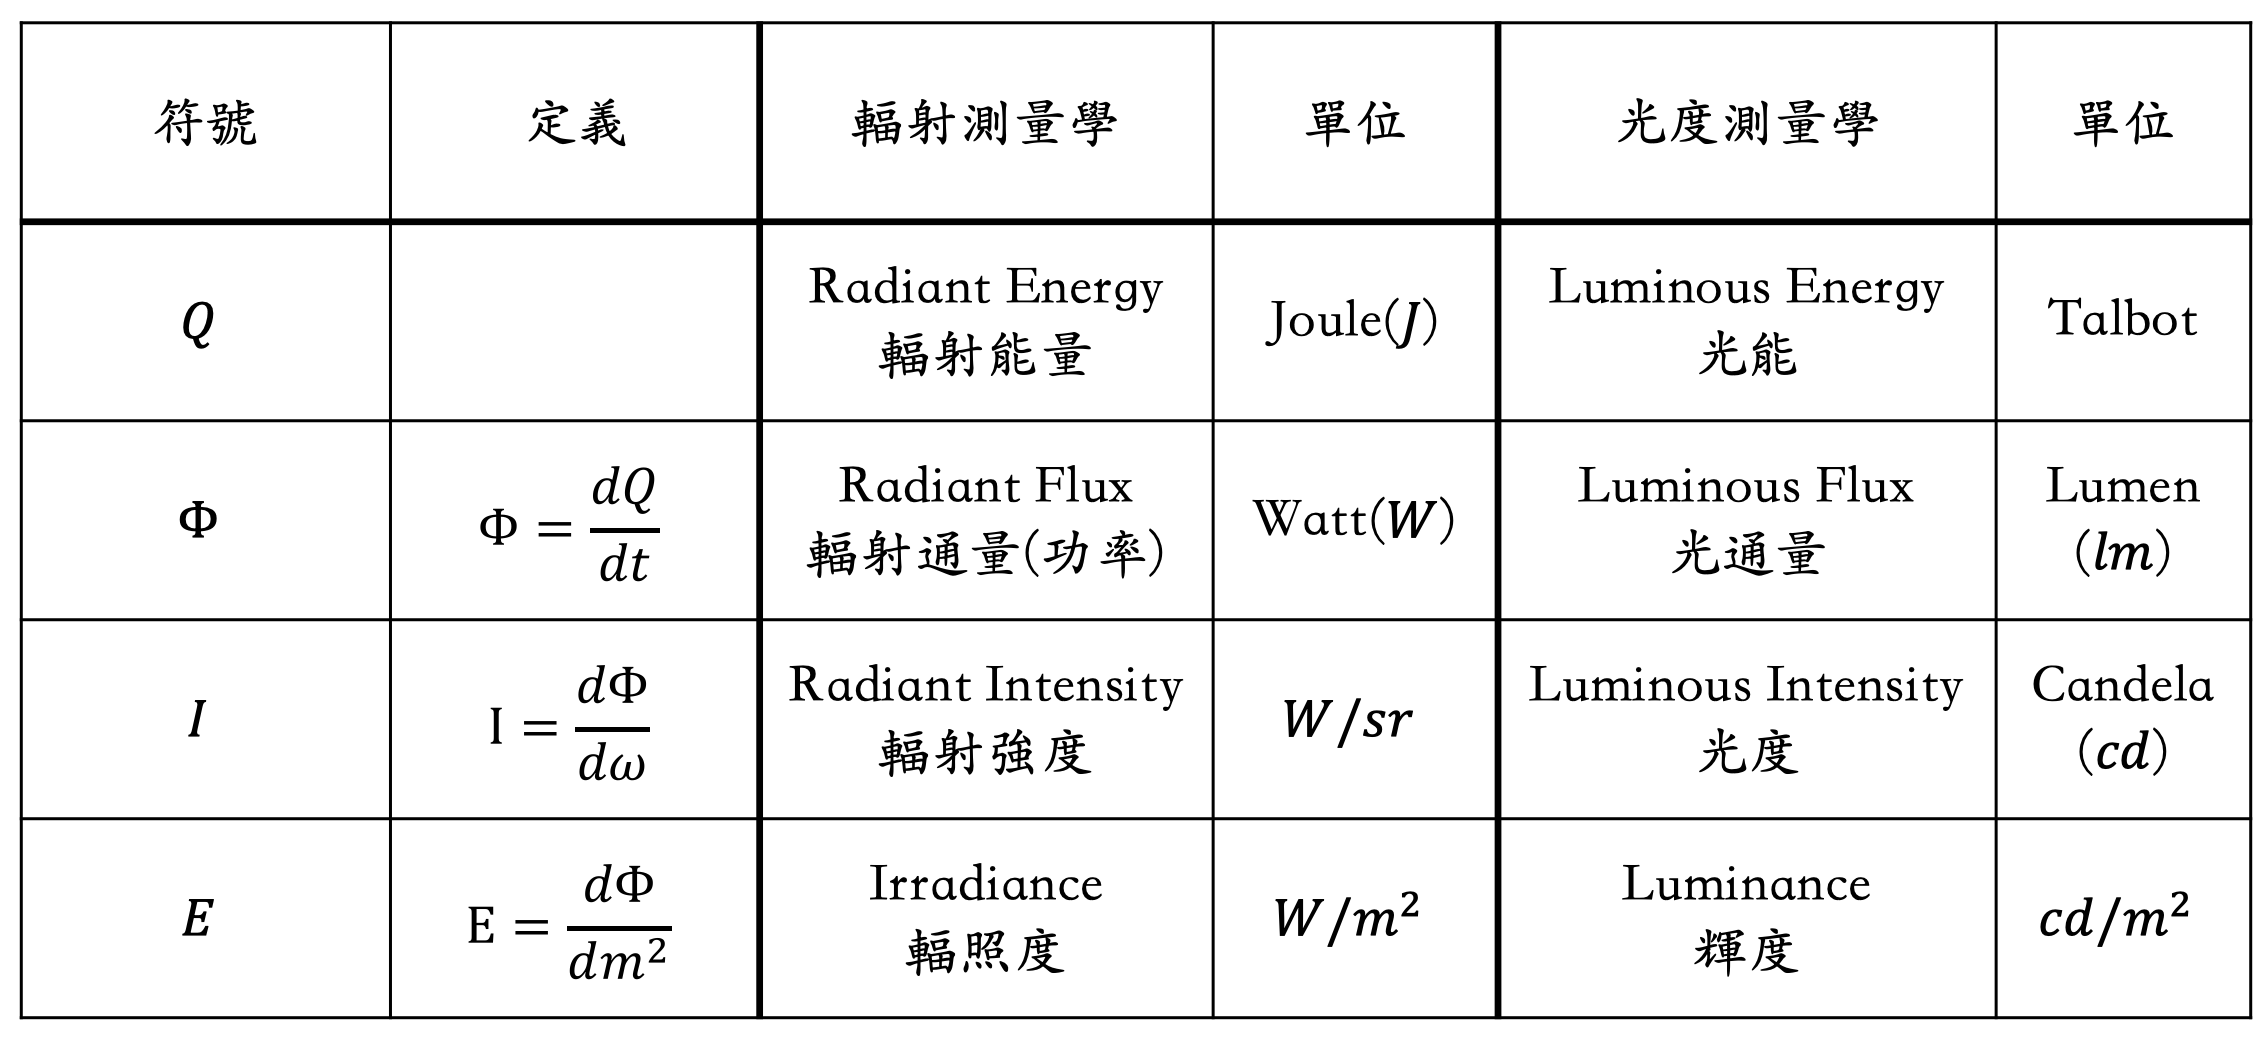
\includegraphics[width=15cm]{ch2pic/photometry_table.png}      
    \end{table}


    本研究聚焦在近紅外光波段,因此本論文會使用輻射測量學的系統,然而文獻上可見光定位數量較多,因此在單位的換算上需特別注意。以下針對光領域常用物理量分項簡單介紹:

    
    \begin{description}
        \item[- 立體角 Solid Angle $\Omega$] \hfill
            
            \qquad
            描述二維空間中的角度單位為弧度,代表夾角內的弧長與半徑比例,而單位弧度的定義是半徑與圓弧長度相等時的圓心角。

            \qquad
            然而光源存在於立體空間中,而空間中描述角度的物理量即為立體角$\Omega$(Solid Angle),該物理量代表一光束投影於單位球面上時,表面積與半徑平方的比例,如圖\ref{pic:solid_angle}所示。立體角的單位為球面度(steradians, 簡寫$sr$)代表在半徑為$r$的球體中,立體角投射出的表面積為$r^2$。

            \begin{figure}[htpb]
                \centering
                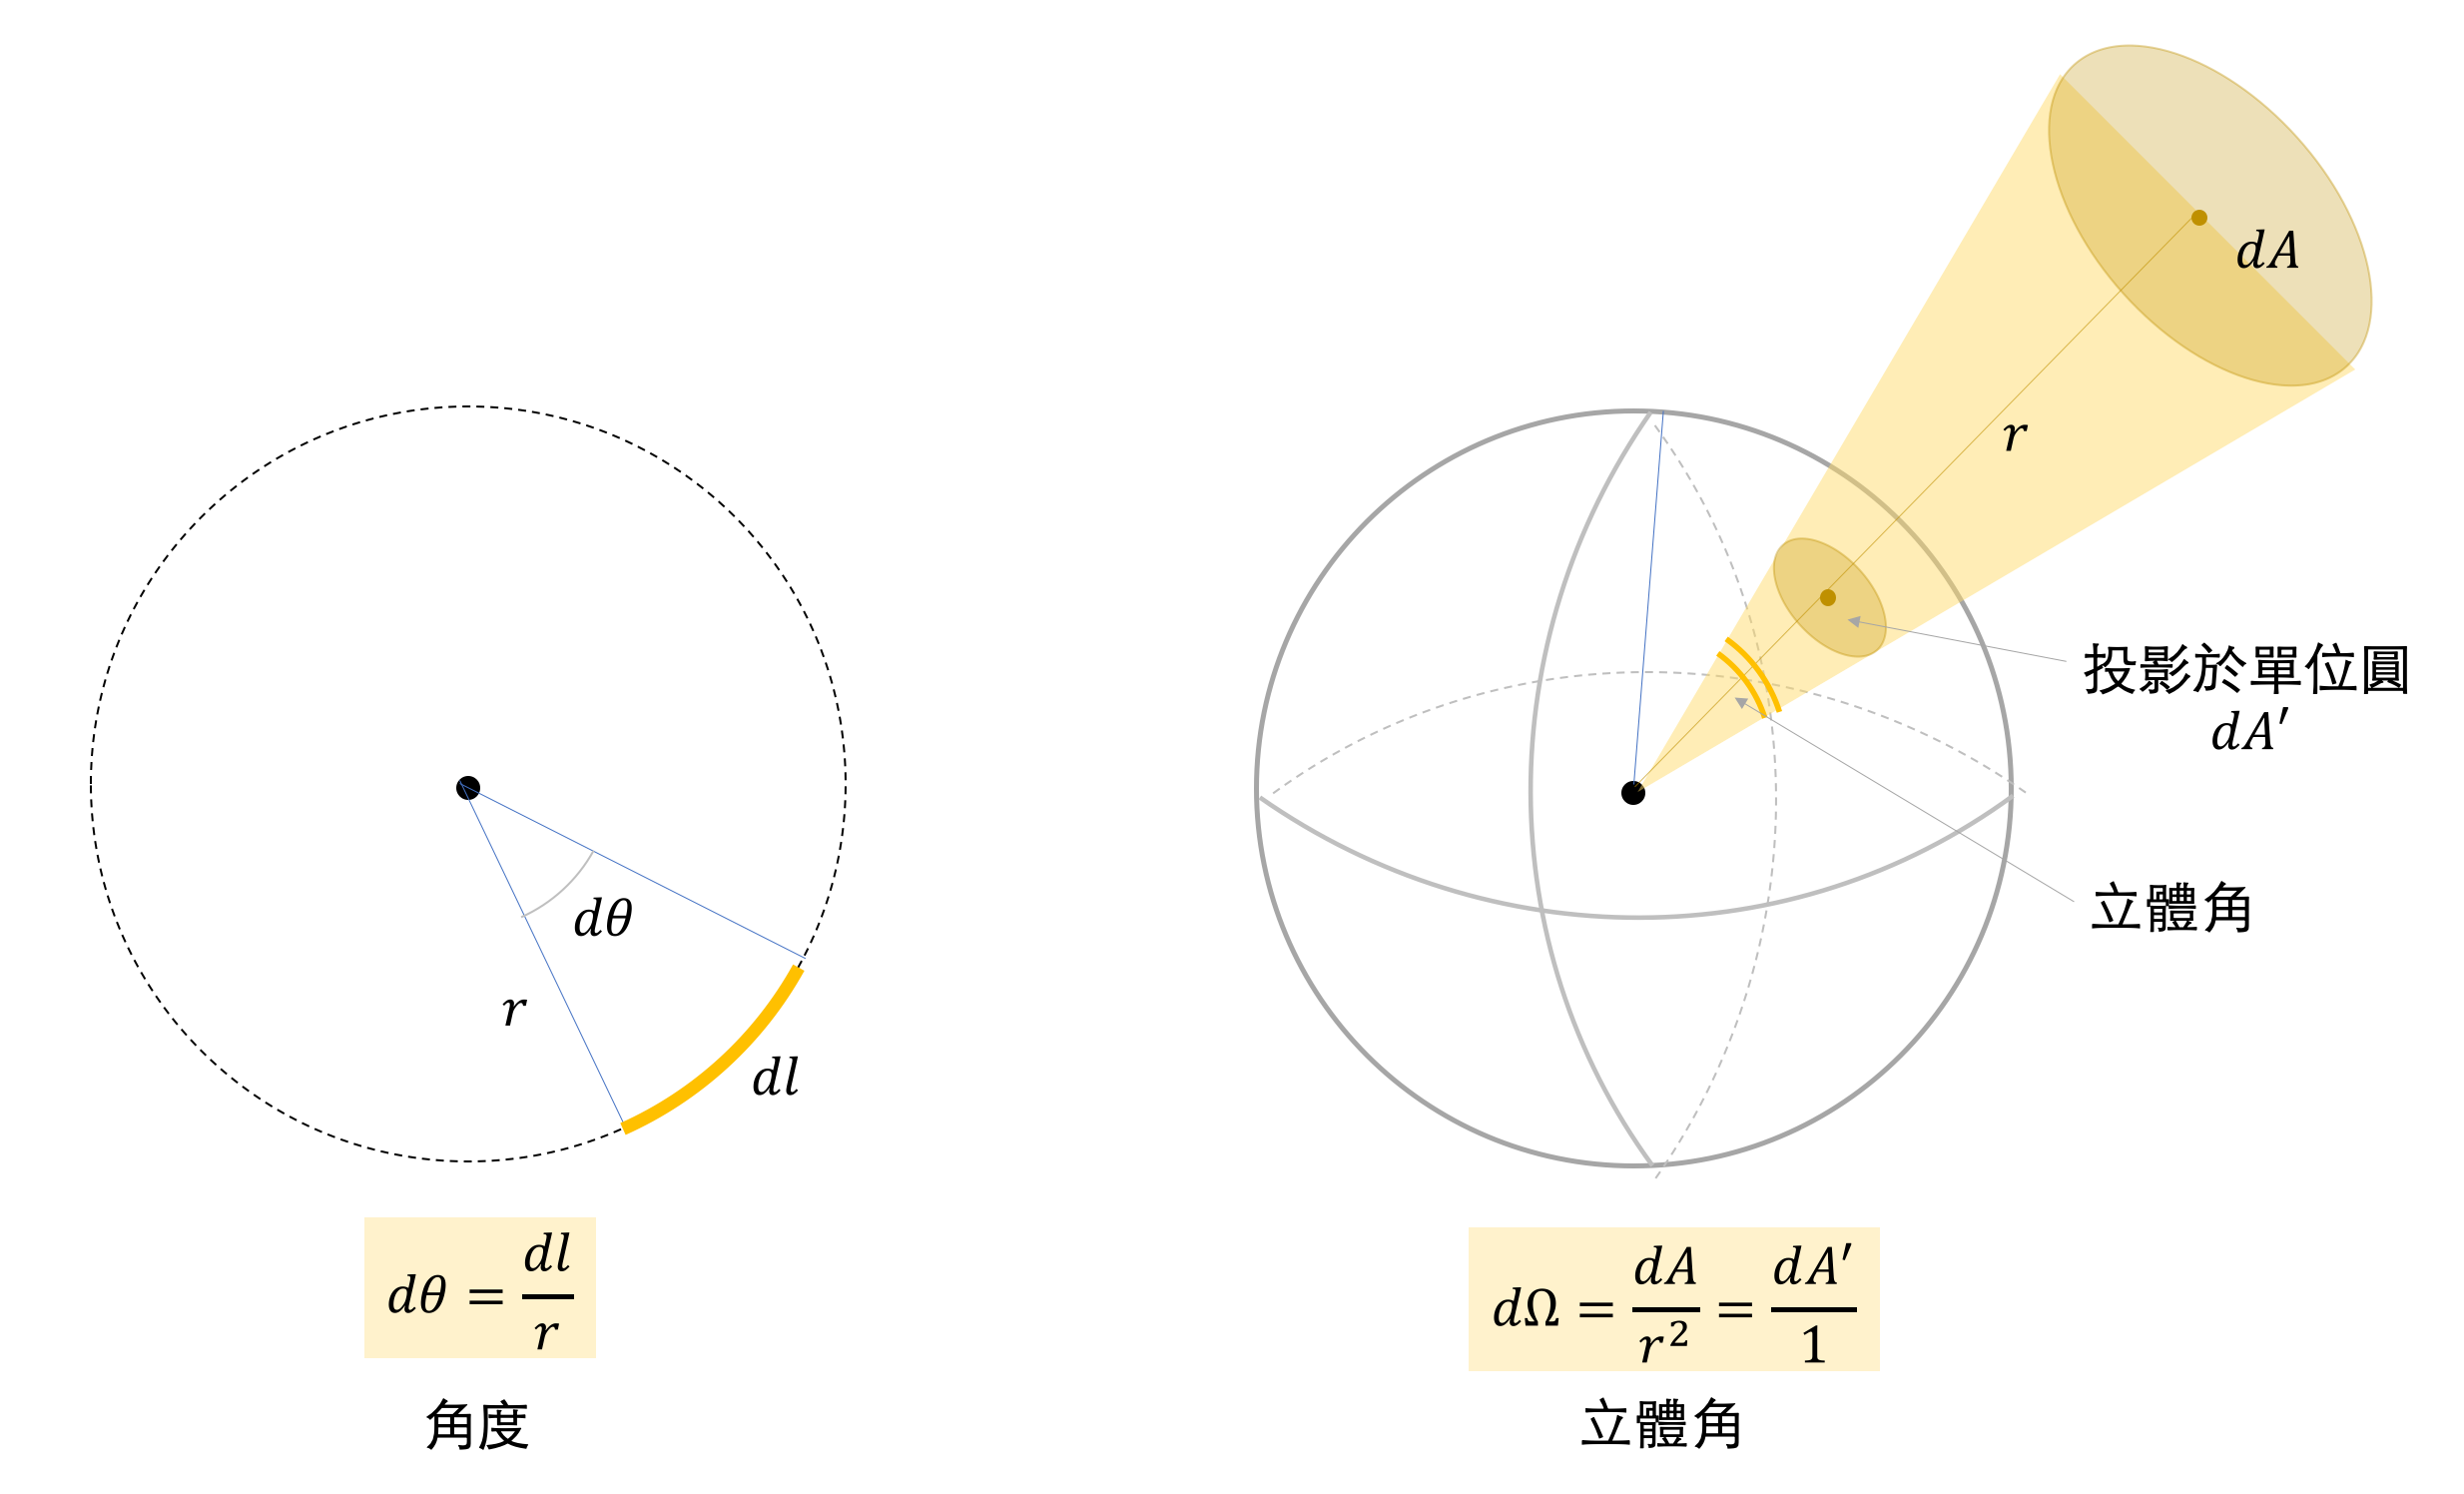
\includegraphics[width=15cm]{ch2pic/solid_angle.png}
                \caption{角度與立體角}
                \label{pic:solid_angle}
            \end{figure}

        \item[- 輻射通量 Radiant Flux $\Phi$]  \hfill
            
            \qquad
            描述光照功率的物理量為通量(Flux)或稱輻射功率(Power),用符號$\Phi$表示,代表每單位時間的輻射能量,單位為瓦特,而大多LED規格表上以此物理量來描述LED在指定電流下可產生的最大光功率。

        \item[- 輻射強度 Radiation Intensity $I$] \hfill
            
            \qquad
            每單位立體角所含的通量稱為輻射強度$I$,此物理量常用於描述光與立體角之關係,在同一光束內,輻射強度僅與立體角有關,與距離無關。

            \begin{figure}[htpb]
                \centering
                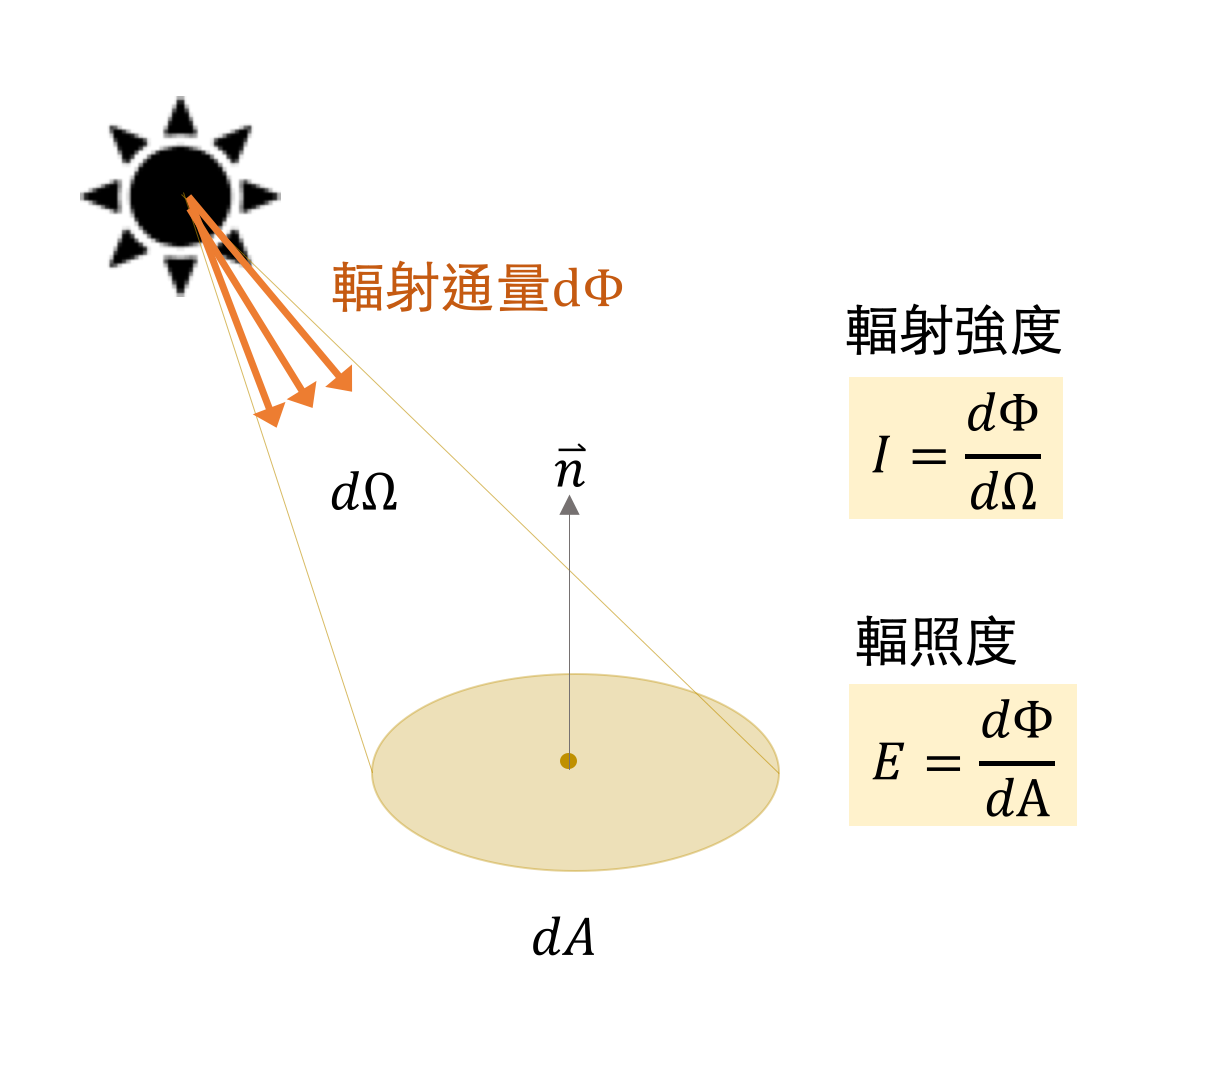
\includegraphics[width=10cm]{ch2pic/intensity_irradiance.png}
                \caption{輻射強度與輻照度}
                \label{pic:intensity_irradiance}
            \end{figure}

        \item[- 輻照度 Irradiance $E$] \hfill
            
            \qquad
            每單位面積所含的通量稱為輻照度(如圖\ref{pic:intensity_irradiance}),其中照射面積隨著距離$D$增加而平方遞增。

            
            % \begin{equation}
            %     \label{eqn:I2E}
            %     E=I\cos\omega/D^2
            % \end{equation}      
            
    \end{description}

    % \subsubsection{LED與PD次系統的規格與特性}
    % \label{chp:LEDPD_character}

    



    
    \subsubsection{朗博輻射模型}
        \label{chp:lambertian}

        \begin{figure}[htpb]
            \centering
            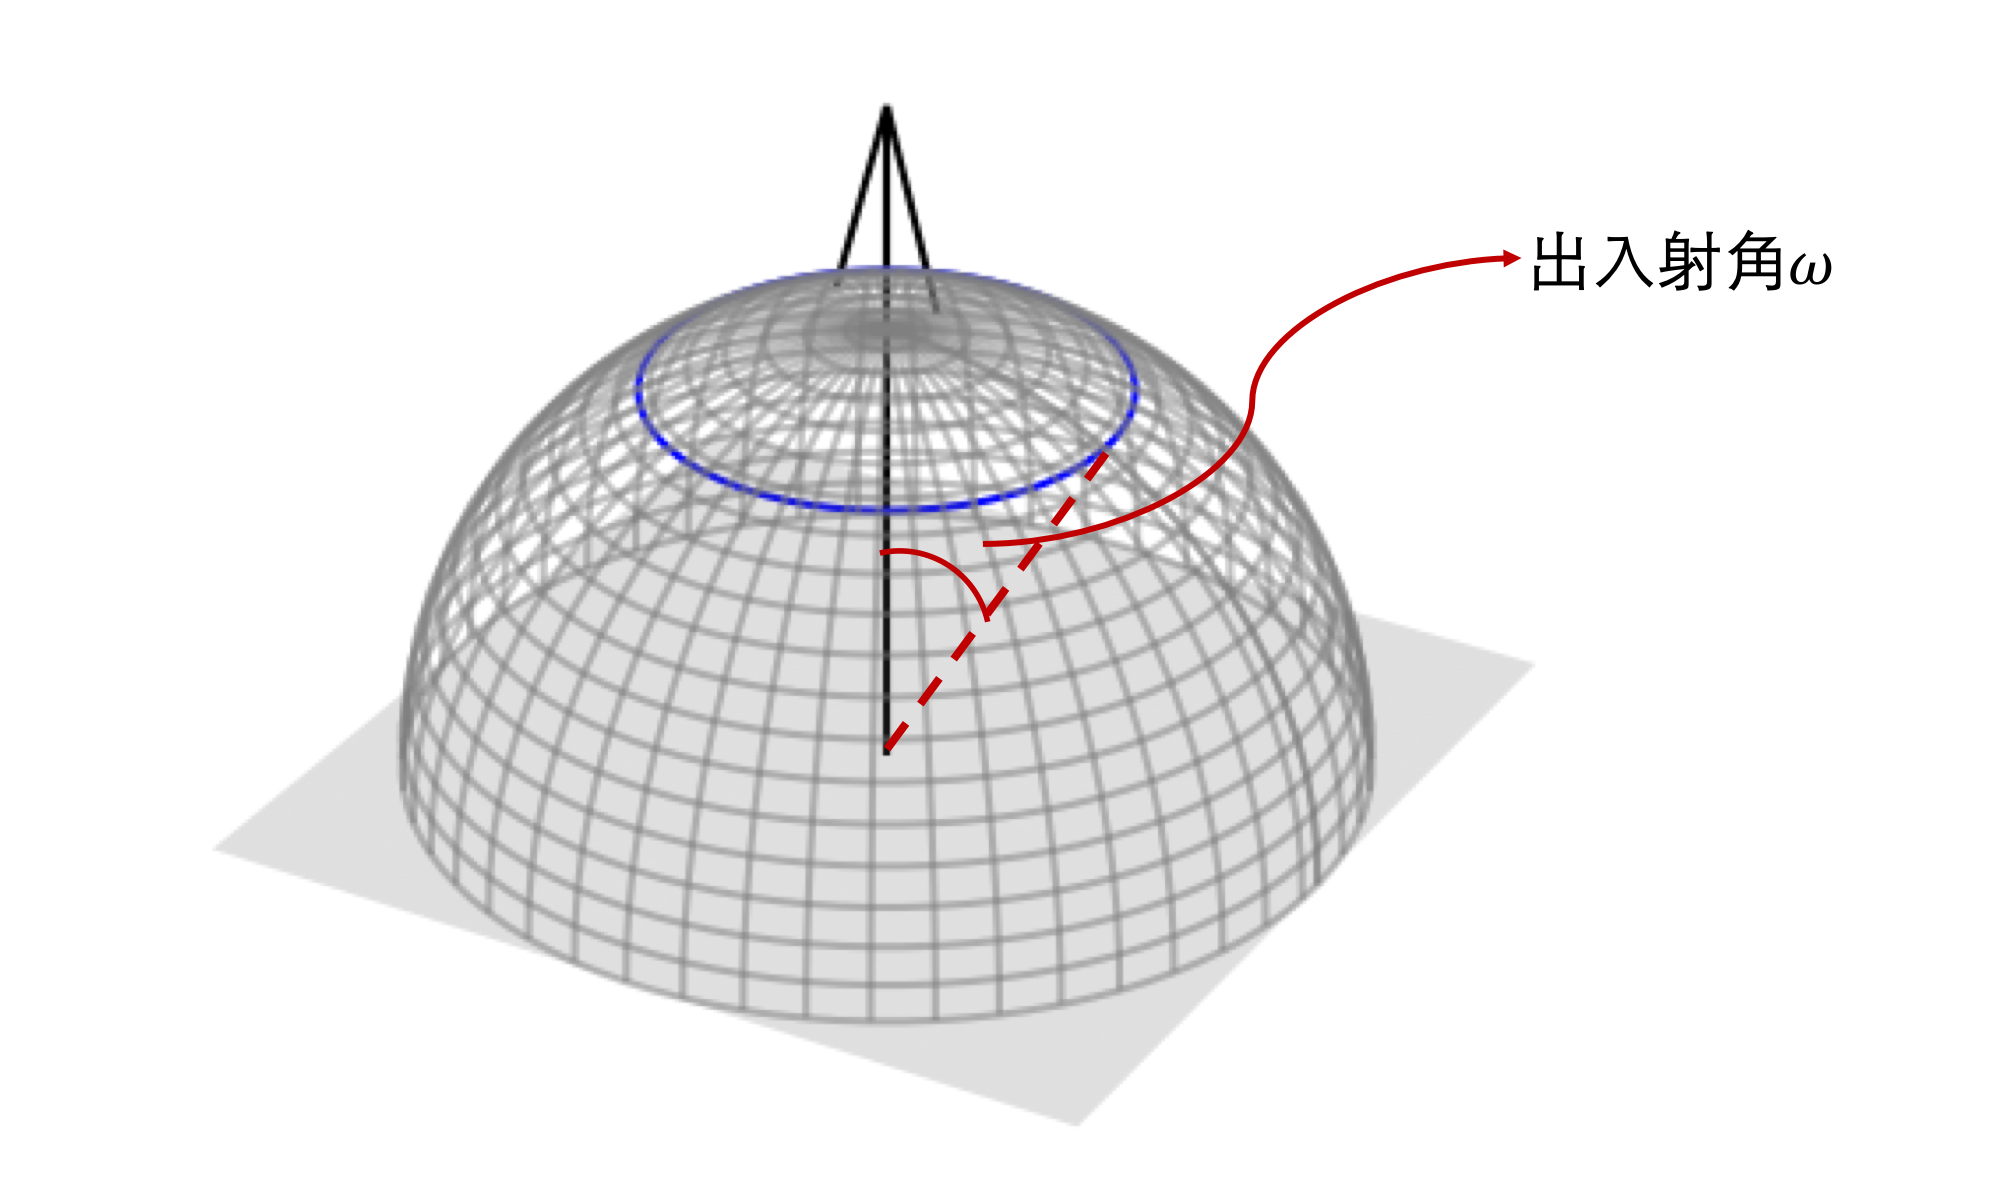
\includegraphics[width=12cm]{ch2pic/3d_angle.png}
            \caption{LED與PD三維空間中的出入射角}
            \label{pic:angle_3d}
        \end{figure}
        

        LED與PD硬體有許多種類,最常見的市面上LED與PD為軸對稱並滿足朗博輻射模式(Lambertian Radiation Pattern),本論文僅考慮此類硬體。其中軸對稱如圖\ref{pic:angle_3d}所示,圖中黑色向量表示硬體指向,輻射強度僅為出入射角$\omega$的函數,而出入射角為硬體指向與出入射角向量之間的夾角;以圖\ref{pic:angle_3d}來看,藍色圓圈上的所有出入射角位置都擁有相同的輻射強度,與方位角無關,呈現軸對稱的特性。

        \begin{figure}[htpb]
            \centering
            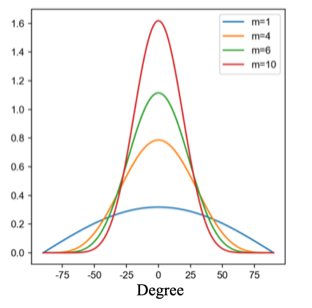
\includegraphics[width=10cm]{ch2pic/lambertian.png}
            \caption{輻射強度與出入射角的關係}
            \label{pic:lambertian}
        \end{figure}

        LED與PD的照射與接收模式(Pattern)皆可以用朗博輻射模式描述(圖\ref{pic:lambertian}),其代表感(發)光強度隨著LED出射角(PD入射角)的增加而衰減,如式\ref{eqn:lambertian_pattern}描述,感(發)光強度於中心軸時最大,其衰減模式可用餘弦函數(cosine)的$M$次方(power)表示,$M$代表的是朗博次方(Lambertian Order),需注意的是輻射強度與距離無關(詳述於\ref{chp:light_unit}章)。

        \begin{equation}
            \label{eqn:lambertian_pattern}
            I(\omega)=I(\omega=0)\times\cos(\omega)^{M}\\
        \end{equation}


        上述為輻射強度與出入射角的關係,為了呈現出入射角於空間中的關係,我們以一向量描述LED與PD的中心軸方位,而由於LED與PD最大的可視範圍不會超過出射角$90^{o}$,因此用半球體描述LED與PD的可視範圍,呈現於圖\ref{pic:angle_3d}。如圖所示,出入射角在空間中僅與球座標系中的天頂角$\alpha$相關,在同樣天頂角時出入射角皆相同。

        以圖\ref{pic:angle_3d}作延伸,空間中的LED與PD,朗博輻射模式在朗博次方為一時如圖\ref{pic:lambertian_3d},在同樣出射角下,光輻射強度相同,呈現軸對稱,愈接近中心軸的輻射強度愈大。

        

        \begin{figure}[htpb]
            \centering
            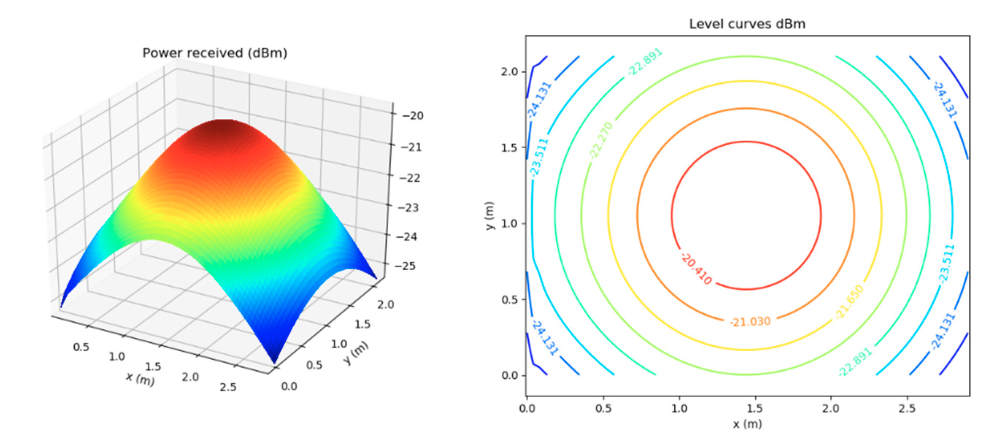
\includegraphics[width=12cm]{ch2pic/lambertian_3d.png}
            \caption{朗博次方為一時空間中輻射強度與出入射角方位的關係}
            \label{pic:lambertian_3d}
        \end{figure}

        而朗博次方所代表的意義,可視為在出入射角角度敏感度與照射範圍中的取捨:朗博次方較小時,其照射範圍較大,最大可以覆蓋半個球表面,光強度隨出射角度衰減的速度不大,也就是對不同入射角度的敏感度不高。反之,朗博次方較大的硬體雖然覆蓋範圍較小,但對覆蓋範圍內的角度變化敏感度高(如圖\ref{pic:lambertian})。因此,硬體的朗博次方是Step1.決定次系統規格中的重要參數,無論是目標物LED次系統還是量測者PD次系統都需要謹慎挑選合適朗博次方的硬體。
        
    \subsubsection{LED與PD的硬體特性}
            \label{chp:LEDPD_hardware}

            LED與PD在選購時,除了挑選朗博次方以外,也需注意其他特性以及影響發收光能力的硬體參數,也屬於Step1.決定次系統規格中的步驟。在此將硬體參數整理於表\ref{pic:hardware_para},以下將LED與PD的特性分項介紹。
            
            \begin{table}[htpb]
                \centering
                \caption{LED與PD的硬體參數}
                \label{pic:hardware_para}
                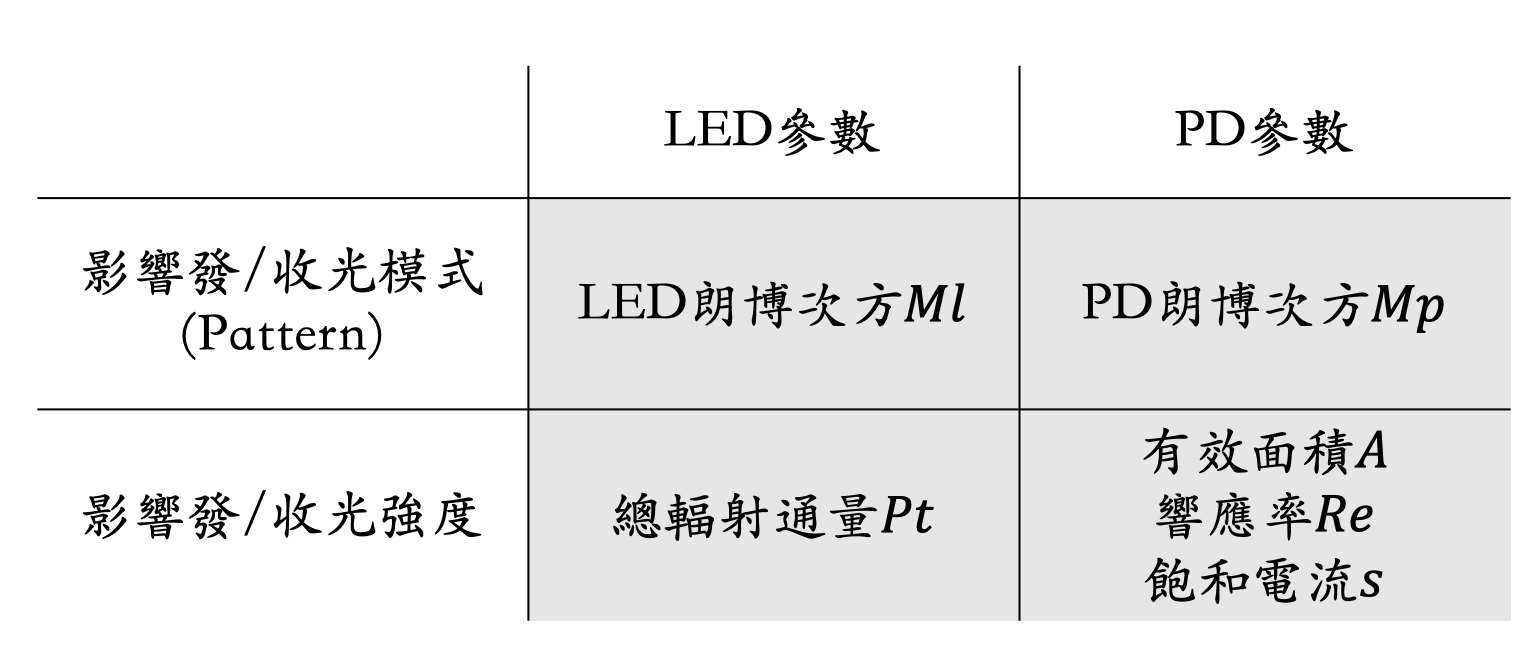
\includegraphics[width=12cm]{ch2pic/hardware_para.png}                
            \end{table}

            \paragraph*{- LED硬體特性}

            \hfill

                LED發出的輻射強度$I\ell$,會遵守式\ref{eqn:lambertian_pattern}描述的朗博輻射模式,其提供了LED光輻射強度$I\ell$與不同出射角$\theta$的關係。而由於描述LED特性時,多以總輻射通量$Pt$描述,而總輻射通量為半球面空間中的輻射強度$I\ell$積分,如式\ref{eqn:lambertian_integral}。

                \begin{equation}
                    \label{eqn:lambertian_integral}
                    Pt = I\ell(0)(M\ell+1)/2\pi
                \end{equation}
                
                \noindent
                透過式\ref{eqn:lambertian_integral}移項與式\ref{eqn:lambertian_pattern},即可完成式\ref{eqn:lambertian_led},描述LED輻射強度$I\ell$與出射角度$\theta$、LED總輻射功率$Pt$以及朗博次方$M\ell$的關係。
            
                \begin{equation}
                    \label{eqn:lambertian_led}
                    I\ell(\theta)=Pt\frac{(M\ell+1)}{2 \pi} \cos \theta^{M\ell}
                \end{equation}

                圖\ref{pic:lambertian_led}呈現了LED在總輻射通量$Pt$相同的情況下,輻射強度$I\ell$與出射角$\theta$的關係。圖中呈現了式\ref{eqn:lambertian_integral}積分的影響,在朗博次方較大時,中心軸的輻射強度比值突出,其原因為朗博輻射模式於半球面上積分的影響。以圖\ref{pic:angle_3d}為例,在半球面上入射角為$0^o$的點僅有與中心軸重疊的位置,相較之下入射角為$90^o$的點則包含z=0平面上半徑為一的整個圓形。由此可知,越大的入射角所含的立體角越大,在擁有固定輻射總通量時,將輻射強度分配給小的立體角度,來分總通量的立體角不多;反之當我們將輻射強度分配給大的入射角度時,入射角大所包含的立體角較多。因此,朗博次方較小時,隨著出入射角度增加,輻射強度衰減速度緩慢,出射角於45度仍有中心軸0.7071倍的強度,因此總通量需分配給大出射角度的部分,所包含的立體角範圍大,使相對輻射強度比值小;而朗博次方較大時,大出射角的輻射強度極小,僅用將總輻射通量分配給小出射角的部分,所含的立體角範圍也小,因此輻射強度對總輻射強度的比值較大。

                \begin{figure}[htpb]
                    \centering
                    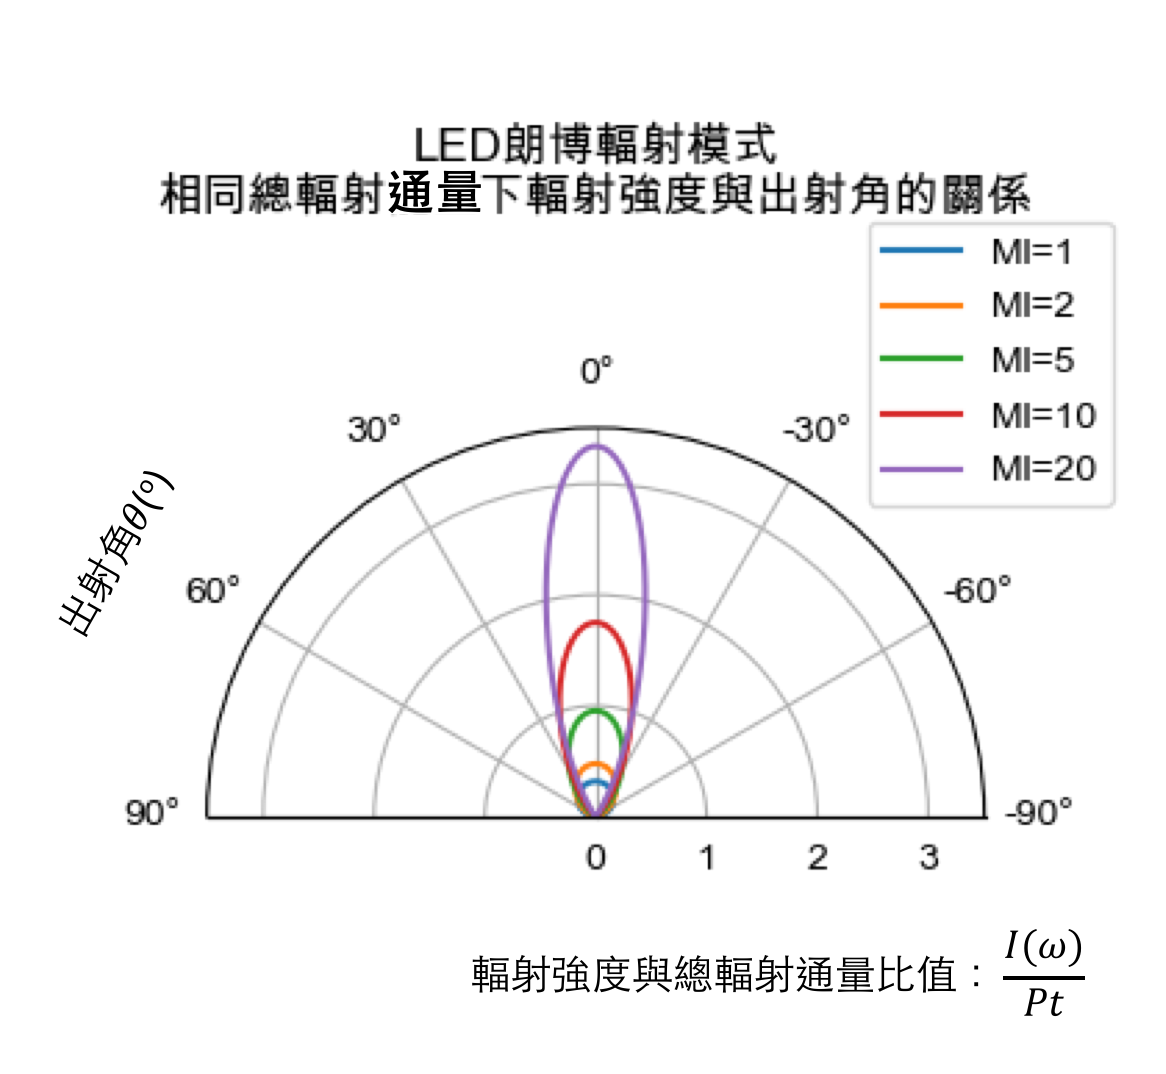
\includegraphics[width=10cm]{ch2pic/lambertian_led.png}
                    \caption{LED輻射強度與總輻射通量比值}
                    \label{pic:lambertian_led}
                \end{figure}




                \paragraph*{- PD硬體特性}

                \hfill
                
                \qquad
                首先,PD得到的輻射強度$Ip$也遵守朗博輻射模式,式\ref{eqn:pd_I}描述輻射強度與入射角度$\phi$以及PD朗博次方$Mp$的關係。

                \begin{equation}
                    \label{eqn:pd_I}
                    Ip(\phi) = Il \cos \phi^{Mp}
                \end{equation}

               \noindent
                而PD所量測到的為輻射通量$\Phi_p$,再將輻射通量轉換為電流輸出(式\ref{eqn:pd_current})。PD量測到的輻射通量呈現於式\ref{eqn:pd_flux},藉由圖\ref{pic:intensity_irradiance}中輻射通量$\Phi$與輻射強度$I$的關係以及立體角$\Omega$的定義,將式\ref{eqn:pd_I}的光強度轉換為PD接收的輻射通量$\Phi p$。其中,$A$為PD的硬體參有效面積,$D$為LED與PD之間的距離。

                \begin{equation}
                    \label{eqn:pd_flux}
                    \Phi p(Ip,D) = \frac{Ip}{\Omega} = \frac{IpA}{D^2}
                \end{equation}

                \noindent
                PD最終輸出電流$Ie$與輻射通量$\Phi p$的關係由式\ref{eqn:pd_current}描述,$s$為PD的飽和電流,也就是該PD能夠輸出的最大電流:在未達飽和之前,輸出電流$Ie$與輻射通量$\Phi p$成正比,比值為響應率$Re$。

                \begin{equation}
                    \label{eqn:pd_current}
                    Ie(\Phi) = \begin{cases}\Phi\times Re, & \text { if } Ie<S \\ S, & \text { otherwise }\end{cases}
                \end{equation}

                \noindent
                綜合式\ref{eqn:pd_I}、式\ref{eqn:pd_flux}、式\ref{eqn:pd_current},PD輸出的電流$Ie$與LED的輻射強度$I\ell$統整於式\ref{eqn:pd},式中的硬體參數如表\ref{pic:hardware_para}:

                \begin{equation}
                    \label{eqn:pd}
                    Ie(D,Il) = \begin{cases}Re \frac{A}{D^2}Il(\theta) \cos \phi^{Mp}, & \text { if } Ie<S \\ S, & \text { otherwise }\end{cases}
                \end{equation}
         

            
            
        

            

    \subsubsection{LED與PD於次系統中的硬體擺設}
        \label{chp:config}


        

        在決定完合適的硬體規格(\ref{chp:LEDPD_hardware}章)後,還需決定LED與PD次系統中的硬體如何擺設,也屬於Step1.決定次系統規格中的步驟。

        \begin{figure}[htpb]
            \centering
            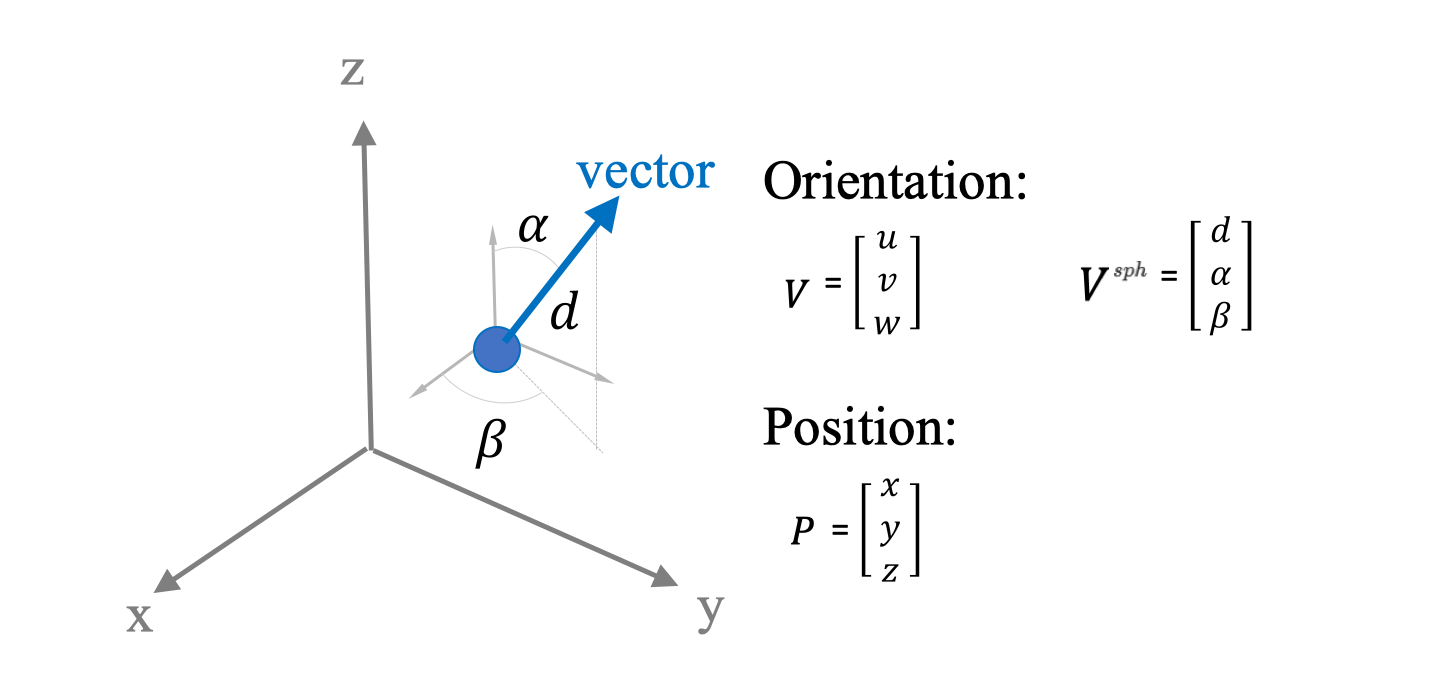
\includegraphics[width=13cm]{ch2pic/vec_config.png}
            \caption{三維空間中的向量}
            \label{pic:vec_config}
        \end{figure}
        
        首先,在描述次系統三維空間中的LED與PD時,需要描述硬體的擺放位置,而由於LED與PD皆有中心軸,因此需要用向量表示指向。如圖\ref{pic:vec_config},圓點代表硬體位置,而向量表示硬體指向,其中位置以$\boldsymbol{P}$表示,包含三個自由度$\left[\begin{array}{ccc}
            x &y&z
            \end{array}\right]^T$,指向則由$\boldsymbol{V}$表示,自由度包含$\left[\begin{array}{ccc}
                u &v&w
                \end{array}\right]^T$,而由於LED與PD指向只在乎方位不在乎距離,因此可將指向向量定義為單位向量:$||\boldsymbol{V}||=1$。指向也常以球座標系表示$\boldsymbol{V}^{sph}$,三個分量為$\left[\begin{array}{ccc}
                    d &\alpha&\beta
                    \end{array}\right]^T$,其中指向的距離分量$d$為一,而球座標系與卡氏座標系之間的換算可如式\ref{eqn:car2sph}。
        

        \begin{figure}[htpb]
            \centering
            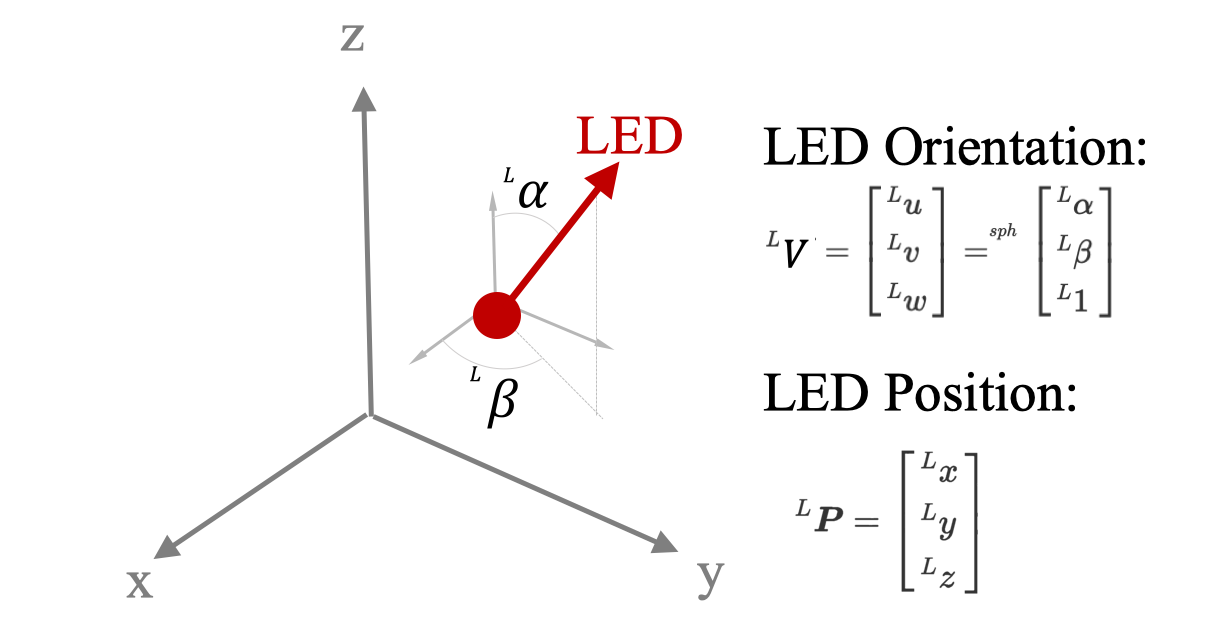
\includegraphics[width=12cm]{ch2pic/LED_config.png}
            \caption{LED在座標系中的擺放自由度}
            \label{pic:led_config}
        \end{figure}

        以LED為例(如圖\ref{pic:led_config}),我們需要定義LED硬體於LED次系統座標系中的位置$^{L}\boldsymbol{P}$與指向$^{L}\boldsymbol{V}$,,左上標$L$代表其定義於LED座標系中。一個LED的組態一共有五個自由度,包含擺放位置$^L \boldsymbol{P}$的三個自由度$\left[\begin{array}{ccc}
            ^Lx &^Ly&^Lz
            \end{array}\right]^T$,以及定義指向的單位向量$^L\boldsymbol{V}$所含兩個自由度:天頂角$^L\alpha$與方位角$^L\beta$,換算至卡氏座標系則為$\left[\begin{array}{ccc}
                ^Lu &^Lv&^Lw
                \end{array}\right]^T$。

        而PD的擺放自由度相同,唯一差別為定義的座標系為PD座標系,因此左上標為$P$,如擺放位置為$^P\boldsymbol{P}=\left[\begin{array}{ccc}
            ^Px &^Py&^Pz
            \end{array}\right]^T$,定義指向的單位向量$^P\boldsymbol{V}=\left[\begin{array}{ccc}
                ^Pu &^Pv&^Pw
                \end{array}\right]^T$。

    \subsubsection{光傳遞模型}
    \label{chp:model}


    本章節將以光傳遞模型描述Step3.LED發送與PD接收訊號中的電流訊號強度,透過綜合\ref{chp:LEDPD_hardware}章中呈現的LED與PD特性,依續介紹由單個LED光源將光波傳送至單個PD,並轉換成電流的完整模型;接著呈現多LED對多PD的光傳遞模型;最後則將光傳播模型中的距離$D$、出入射角$\theta\phi$變數轉換為用LED與PD的次系統座標系表示。
            
        % \subsubsection{單LED對單PD光傳遞模型}
    \paragraph*{- 單LED對單PD光傳遞模型}
        % \label{chp:model_1to1}

        \hfill
    
        光傳遞模型需建立由LED至PD的過程,LED與PD各自的輻射與接收特性可如\ref{chp:LEDPD_hardware}章中的介紹,綜合描述LED發光強度$Il$的式\ref{eqn:lambertian_led},以及描述PD輸出電流$Ie$的式\ref{eqn:pd},即可獲得一LED對一PD的光傳遞模型(式\ref{eqn:model_1to1})。
    
        \begin{equation}
            \label{eqn:model_1to1}
            Ie(D,\theta,\phi) = \begin{cases}Re \cdot A\cdot Pt\frac{M\ell+1}{2\pi}\frac{\cos \phi^{Mp}\cos \theta^{M\ell}}{D^2}, & \text { if } Ie<S \\ S, & \text { otherwise }\end{cases}
        \end{equation}
    
        在光傳遞模型中,與定位相關的變數包含三個:距離$D$、PD入射角$\phi$、LED出射角$\theta$,他們便是幾何方法演算法要使用的三個變數。其中出入射角如圖\ref{pic:interactive_1to1},分別為硬體中心軸與距離向量之間的夾角。
    
        \begin{figure}[htpb]
            \centering
            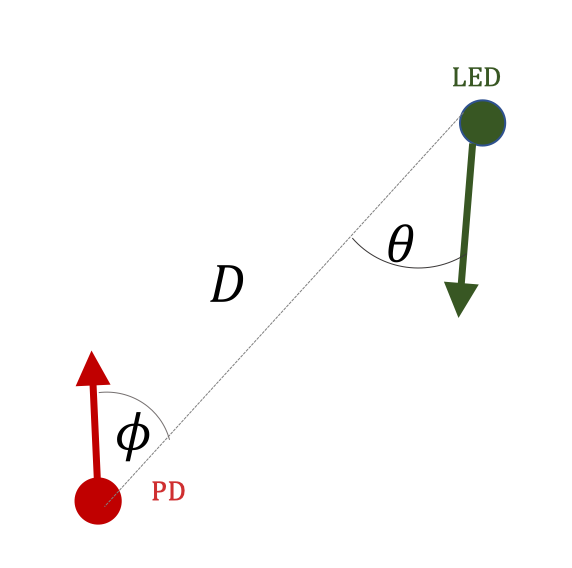
\includegraphics[width=5cm]{ch2pic/interactive_1to1.png}
            \caption{單LED與單PD的交互關係}
            \label{pic:interactive_1to1}
        \end{figure}

        \paragraph*{- 多LED對多PD光傳遞模型}
        % % \subsubsection{多LED對多PD光傳遞模型}
        % \label{chp:model_mul}

        \hfill
    
        由於LED與PD定位時數量通常不只一個,因此描述多LED對多PD的光傳遞模型時,需註明清楚(可參考第\pageref{chp:symbol}頁)。在此設定LED總數為$L$、PD總數為$P$,描述第$l$個LED與第$p$個PD的硬體參數時,於硬體參數的右下標加註,如$A_2$為第二個PD的有效面積;再來,描述第$l$個LED與第$p$個PD之間的交互幾何關係時,則將LED與PD的編號$lp$同樣加註於右下標,例如$D_{34}$為第三個LED與第四個PD之間的距離,如圖\ref{pic:interactive_mul}。
        
        \begin{figure}[htpb]
            \centering
            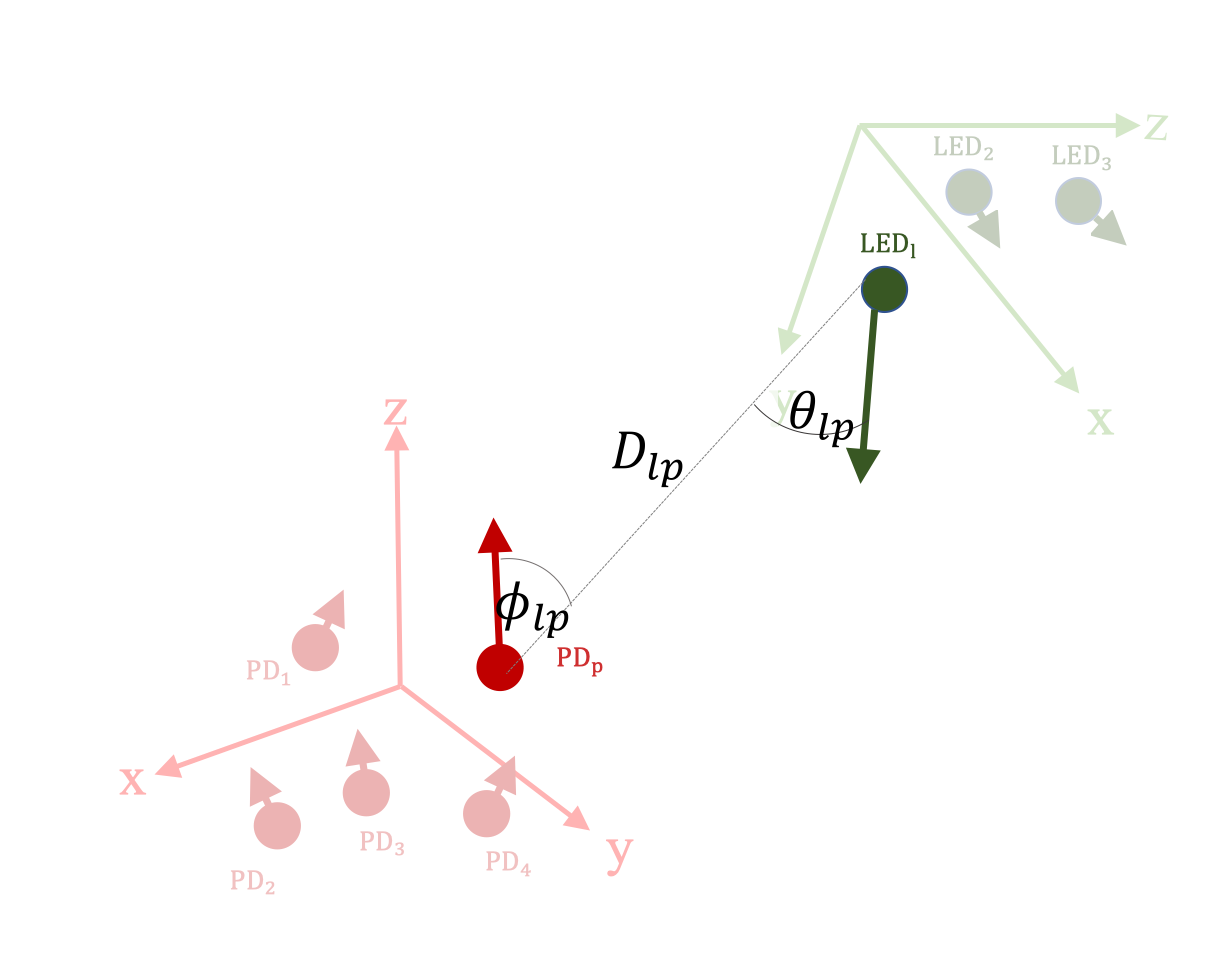
\includegraphics[width=12cm]{ch2pic/interactive_mul.png}
            \caption{多LED與多PD的交互關係}
            \label{pic:interactive_mul}
        \end{figure}
    
        而完整的多LED對多PD的的模型如式\ref{eqn:model},$Ie_{lp}$代表著第$p$個PD收到來自第$l$個LED所產生的電流大小。
        
        \begin{equation}
            \label{eqn:model}
            Ie_{lp}(D_{lp},\theta_{lp},\phi_{lp}) = \begin{cases}Re_p \frac{ A_p\cos\phi_{lp}^{Mp_{p}} }{D^2_{lp}}\times Pt_l\frac{(M\ell_{l}+1)}{2 \pi} \cos \theta_{lp}^{M\ell_{l}}, & \text { if } Ie_{lp}<S_p \\ S_p, & \text { otherwise }\end{cases}
        \end{equation}
    
        
    
    
    
    
        \paragraph*{- 以兩次系統座標之間相對關係為變數的光傳遞模型}
        % \label{chp:model_transform}

        \hfill
    
        雖然式\ref{eqn:model}已呈現了多LED對多PD的光傳遞模型,然而式子中的變數為距離$D_{lp}$與出入射角$\theta_{lp},\phi_{lp}$,如圖\ref{pic:relative_vs_coor},這三個變數為LED與PD各自於全域座標系中的交互幾何關係,並沒有將LED與PD定義於各自的次系統座標系中,呈現\ref{chp:relative}章中描述的兩次系統座標系各自移動的情境。而由於Step1.決定次系統規格中的硬體擺設方式都是定義於各自次系統座標系中,我們為了得到Step2.系統設置中兩次系統座標系相對位置,與Step3.PD接收電流強度之間的關係,因此需要將式\ref{eqn:model}中的三個全域座標系中的幾何變數$D_{lp},\phi_{lp},\theta_{lp}$,改以兩座標系轉換關係與硬體於次系統座標系中的擺設來表示,才能夠利用電流強度$Ie_{lp}$得到兩次系統之間的相對位置$^{PL}\boldsymbol{T}$關係。
    
        \begin{figure}[htpb]
            \centering
            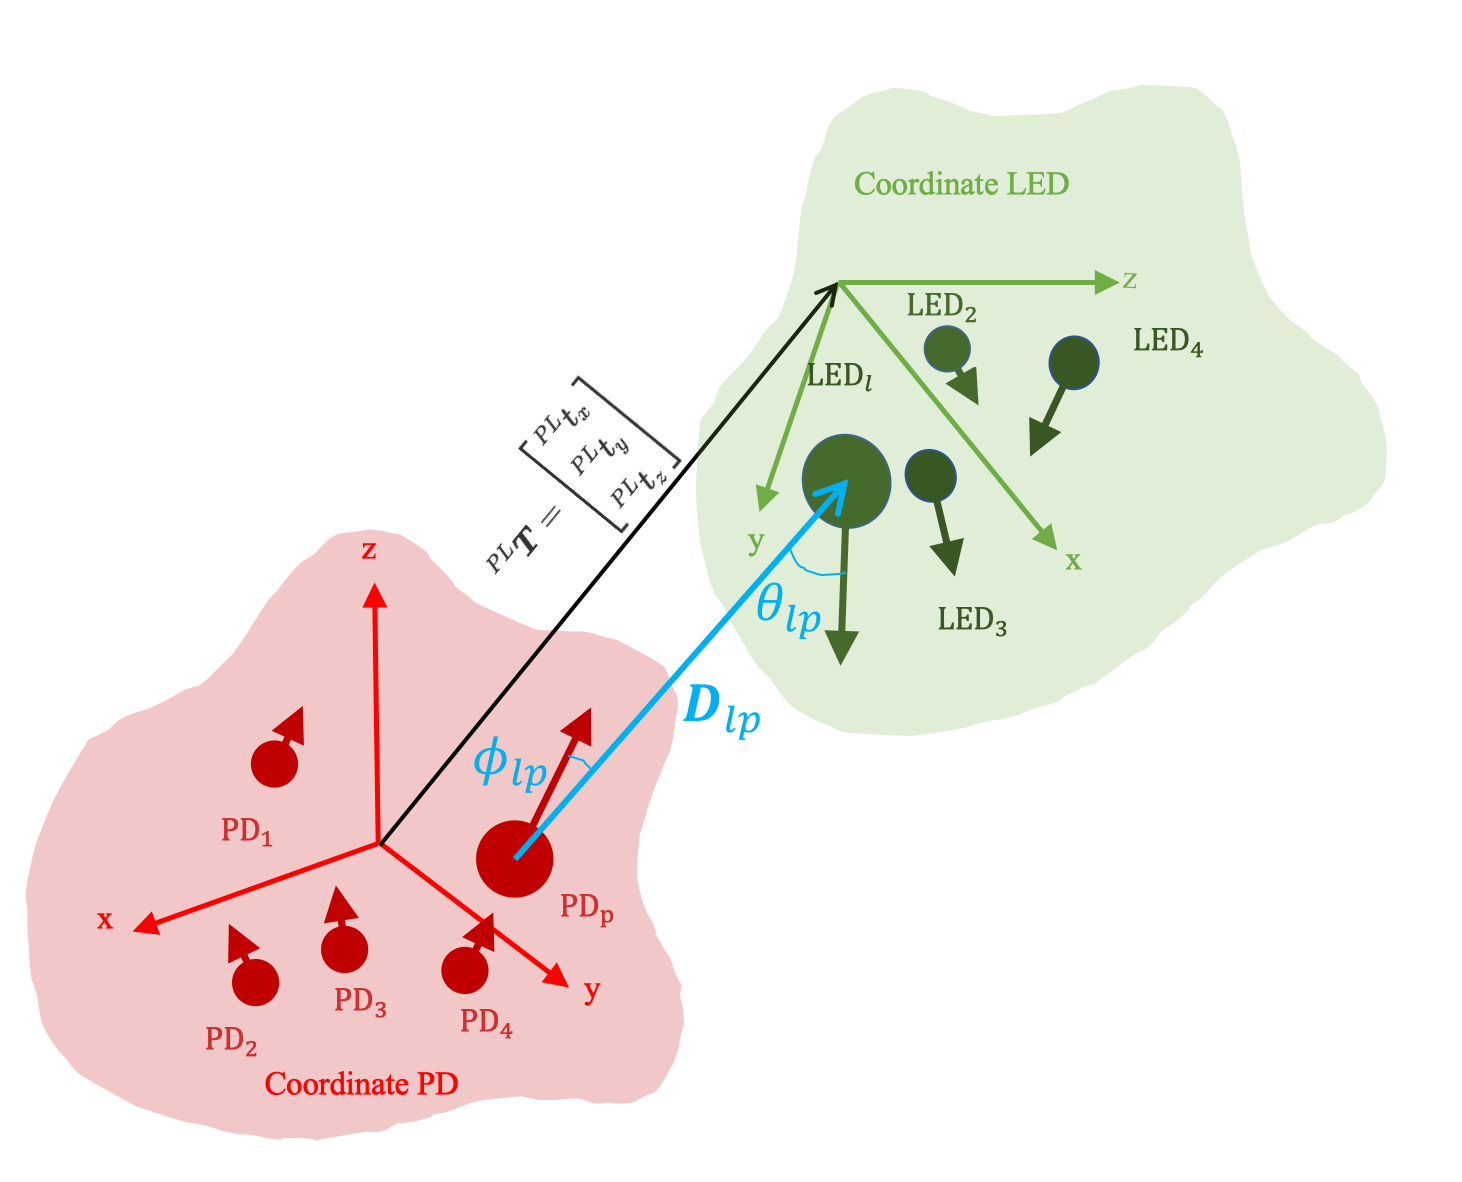
\includegraphics[width=15cm]{ch2pic/relative_vs_coor.png}
            \caption{LED與PD次系統中座標系的LED與PD交互關係}
            \label{pic:relative_vs_coor}
        \end{figure}
    
        為了達到此目的,以下,我們需先獲得兩次系統座標系上的硬體,於全域座標系中的幾何交互關係:$D,\theta,\phi$,此步驟中需將LED次系統座標系中的硬體擺設位置$\boldsymbol{P}$與指向$\boldsymbol{V}$,透過\ref{chp:relative}章中定義的齊次座標轉換矩陣$^{PL}\boldsymbol{H}$投影至PD次系統座標系上,於PD座標系中計算幾何交互關係。接著,透過以次系統座標表示的幾何交互關係$D,\theta,\phi$,即可帶入光傳遞模型中取得以次系統座標系相對關係為變數的光傳遞模型。
        
        
 
        % \end{figure}
        
        % \begin{description}
    
        %     \item[A. 次系統座標系相對關係呈現硬體幾何交互關係$D,\theta,\phi$]
            
        %     \hfill

        %     \begin{description}

        %     \item[a. 將LED次系統中的硬體擺設投影到PD座標系上]\hfill 
            
        %         \qquad
                首先是LED位置$^L \boldsymbol{P}_l$與指向$^L \boldsymbol{V}_l$需由LED次系統座標系中投影至PD座標系上,我們透過式\ref{eqn:homogeneous_point}將$^L \boldsymbol{P}_l$經過齊次座標轉換至PD座標系上,以$^{PL} \boldsymbol{P}_l$描述被投影至PD座標系上的LED位置。而$^L \boldsymbol{V}$為單位指向向量,僅用旋轉矩陣$\boldsymbol{Ro}$轉換投影至PD座標系上如式\ref{eqn:homogeneous_vector},$^{PL}\boldsymbol{V}$描述被投影至PD座標系上的LED指向。
        
                \begin{equation}
                    \label{eqn:homogeneous_point}
                    \begin{aligned}
                    \left[\begin{array}{cc}
                    { }^{P L} \boldsymbol{P} \\
                    1
                    \end{array}\right]&={ }^{P L} \boldsymbol{H}\left[\begin{array}{c}
                    { }^{L} \boldsymbol{P} \\
                    1
                    \end{array}\right] &=\left[\begin{array}{cc}
                    { }^{P L} \boldsymbol{R} \boldsymbol{o} & { }^{P L} \boldsymbol{T} \\
                    0 & 1
                    \end{array}\right]\left[\begin{array}{c}
                    { }^{L} \boldsymbol{P} \\
                    1
                    \end{array}\right] \\
                \end{aligned}
                \end{equation}
                
                \begin{equation}
                    \label{eqn:homogeneous_vector}
                    \begin{aligned}
                    ^{P L} \boldsymbol{V} &=^{P L} \boldsymbol{R} \boldsymbol{o} ^{L}\boldsymbol{ V} 
                    \end{aligned}
                \end{equation}
    
    
    
    
                % \item[b. 於PD座標系中計算各LED與PD之間的距離、出入射角]\hfill 
                
                %     \qquad
                \noindent
                    有了在同一個PD座標系中的LED與PD位置和指向,則可以利用兩硬體位置相減,以式\ref{eqn:distance_to_coor}計算第$l$個LED與第$p$個PD之間的距離向量$\boldsymbol{D}_{lp}$,向量以粗體表示,距離純量大小則以${D}_{lp}$表示。
                    
                    \begin{equation}
                        \label{eqn:distance_to_coor}
                        \begin{aligned}
                        \boldsymbol{D}_{lp} = ^{PL}\boldsymbol{P}_l- ^{P}\boldsymbol{P}_p \\
                        D_{lp} = ||\boldsymbol{D}_{lp}||
                        \end{aligned}
                    \end{equation}
            
                    \noindent
                    再來,第$l$個LED對第$p$個PD出射角$\theta_{lp}$與入射角$\phi_{lp}$,可透過餘弦與內積的關係求得,於式\ref{eqn:angle_to_coor}表示。
            
                    \begin{equation}
                        \label{eqn:angle_to_coor}
                        \begin{aligned}
                        \theta_{lp} = \arccos(-\frac{^{PL}\boldsymbol{V}_l \cdot {\boldsymbol{D}_{lp}}}{D_{lp}})\\
                        \phi_{lp} = \arccos(\frac{^{P}\boldsymbol{V}_p \cdot {\boldsymbol{D}_{lp}}}{D_{lp}})\\
                        \end{aligned}
                    \end{equation}
            %     \end{description}
    
            % \item[B. 將次系統座標系相對關係呈現硬體幾何交互關係帶入光傳遞模型]\hfill
            
            %     \qquad
                將距離、出入射角三個幾何交互關係,都以兩座標系之間的相對關係作為變數表示後,於式\ref{eqn:model_coor}將整個光傳播模型(式\ref{eqn:model})以兩座標系之間的相對關係作為變數表示:
        
                \begin{equation}
                    \label{eqn:model_coor}
                    \begin{aligned}
                        \text { if } Ie_{lp}<s_p \\
                        Ie_{lp} &= \frac{Re_pA_pPt_l(M\ell_{l}+1)}{2 \pi} \frac{ {\cos\phi_{lp}}^{Mp_{p}} \times{\cos \theta_{lp}}^{M\ell_{l}}}{D^2_{lp}}\\
                            & = \frac{Re_pA_pPt_l(M\ell_{l}+1)}{2 \pi} \frac{ {{(^{P}\boldsymbol{V}_p \cdot {\boldsymbol{D}_{lp}})}}^{Mp_{p}} {(-^{PL}\boldsymbol{V}_l \cdot {\boldsymbol{D}_{lp}})}^{M\ell_{l}}}  {{||{\boldsymbol{D}_{lp}}||}^{2+M\ell_l+Mp_p}}
                    \end{aligned}
                \end{equation}
        
                \noindent
                其中,${\boldsymbol{D}_{lp}}$、$||{\boldsymbol{D}_{lp}}||$、$^{PL}\boldsymbol{V}_l$都還未完全展開,我們將其完全展開呈現於式\ref{eqn:model_coor_extend}。
        
        
                \begin{equation}
                    \label{eqn:model_coor_extend}
                    \begin{aligned}
                        &\text { if } Ie_{lp}<s_p \\
                        &Ie_{lp}(^{PL}\boldsymbol{T},^{PL}\boldsymbol{Ro}) \\&= \frac{Re_pA_pPt_l(M\ell_{l}+1)}{2 \pi} 
                        \\
                        &\qquad \times
                            \frac{ 
                            {(
                                ^{P}\boldsymbol{V}_p 
                                \cdot 
                                (
                                    ^{PL}\boldsymbol{P}_l- ^{P}\boldsymbol{P}_p
                                )
                            )}
                            ^{Mp_{p}}
                            \times 
                            {(
                                -^{PL}\boldsymbol{Ro}^{L}\boldsymbol{V}_l 
                                \cdot 
                                ({
                                    ^{PL}\boldsymbol{P}_l
                                    - ^{P}\boldsymbol{P}_p
                                })
                            )}^{M\ell_{l}}
                        } 
                            {{||^{PL}\boldsymbol{P}_l- ^{P}\boldsymbol{P}_p||}^{2+M\ell_l+Mp_p}}\\
                            &= \frac{Re_pA_pPt_l(M\ell_{l}+1)}{2 \pi}\\
                            &\qquad\times 
                            {( ^{P}\boldsymbol{V}_p \cdot 
                                    (
                                        (
                                            ^{PL} \boldsymbol{Ro}^{P}\boldsymbol{P}_l
                                            + ^{PL}\boldsymbol{T}
                                        )
                                        - ^{P}\boldsymbol{P}_p
                                    )
                                )}^{Mp_{p}}\\
                        &\qquad\times
                        {
                                    (
                                        -^{PL}\boldsymbol{Ro}^{L}\boldsymbol{V}_l 
                                        \cdot 
                                        (
                                            (
                                                ^{PL}\boldsymbol{Ro}^{P}\boldsymbol{P}_l
                                                +^{PL}\boldsymbol{T}
                                            )
                                            - ^{P}\boldsymbol{P}_p
                                        )
                                    )
                                }^{M\ell_{l}}   \\
                        & \qquad \times
                            \frac{     
                                1   
                            } 
                            {
                                {
                                    ||
                                        (^{PL}\boldsymbol{Ro}^{P}\boldsymbol{P}_l+^{PL}\boldsymbol{T})
                                        - ^{P}\boldsymbol{P}_p
                                    ||
                                }^{2+M\ell_l+Mp_p}
                            }\\
                    \end{aligned}
                \end{equation}
    
        % \end{description}   
    
    
            
        透過式\ref{eqn:model_coor_extend},我們已經將Step3.LED發送與PD接收訊號步驟中PD量測到的電流訊號強度,以兩次系統座標系之間的相對關係$^{PL}\boldsymbol{T}$、$^{PL}\boldsymbol{Ro}$描述,而由式中的複雜度我們可以進而得出結論:無論是硬體擺設方式$\boldsymbol{P}$或$\boldsymbol{V}$改變,亦或是兩座標系相對關係$^{PL}\boldsymbol{H}$改變,皆會影響到輸出電流,是一個牽一髮動全身的模型,我們難以輕易透過輸出電流,獲得相對位置$^{PL}\boldsymbol{T}$。\textbf{因此,所有的研究皆需利用不同的限制方式,使式\ref{eqn:model_coor}簡化,以取得相對位置資訊}。
    
    
    
    
    
        
        


\subsection{現行LED與PD的定位方法與應用}
\label{chp:LEDPD_now}
            


由於\ref{chp:model}章中呈現的光傳遞模型,在完整考慮Step1.中的硬體擺設自由度與硬體規格的選擇,以及Step2.系統設置時兩次系統座標系六個自由度的相對關係時,會使模型非常複雜如式\ref{eqn:model_coor_extend},難以從中獲得PD電流強度與相對位置$^{PL}\boldsymbol{T}$的關係。因此現有文獻都會透過適當限制Step1.與Step2.的自由度以簡化模型,常見限制於\ref{chp:LEDPD_restrict}章中介紹,而在\ref{chp:LEDPD_case}章中則介紹幾個與本研究較相近的文獻的定位方法。

    \subsubsection{常見的次系統規格與系統設置的限制}
    \label{chp:LEDPD_restrict}

    現今文獻需加諸系統限制以求得兩次系統之間的相對位置,而常見的限制以下條列呈現:

    

    \begin{description}
        \item[$\cdot$ 忽略朗博次方] \hfill
        
        \qquad
        朗博次方是一個影響輻射模式的重要參數(如\ref{chp:lambertian}章),LED與PD兩者皆有各自的朗博次方,代表著訊號對角度敏感度與覆蓋範位的取捨。大多文獻將LED與PD的朗博次方皆假設為一,降低系統複雜度,使式\ref{eqn:model_coor_extend}簡化於式\ref{eqn:model_no_lamb}。

        \qquad
        然而,假設朗博次方為一在實際上是不符合現實的,因為實際上在挑選硬體時朗博次方時有許多選擇,如\cite{datasheet:led_vsma}的朗博次方約為5.57。為了降低複雜度而省略朗博次方,會侷限Step1.決定次系統規格時能夠挑選使用的硬體,也限制了系統的自由度\cite{survey_light2018}。即便如此,大多研究仍將其省略,其中將PD的朗博次方納入考量的文獻極少\cite{survey_light2018},相較起來,LED朗博次方有少部分研究將其納入計算,如\cite{case:cart2d}\cite{case:cart3d}。
        
        

        \item[$\cdot$ 硬體種類限制]\hfill
        
        \qquad
        文獻上,在Step1.決定次系統規格中的硬體規格時,$L$個LED皆會選擇同一規格,也就是同一系統下,並不會出現不同規格的LED,PD亦然。因此,LED與PD的硬體參數(如表\ref{pic:hardware_para})並不會隨LED與PD的編號改變,綜合此限制與朗博次方為一的限制,將式\ref{eqn:model_coor_extend}簡化為式\ref{eqn:model_no_lamb}。

        \begin{equation}
            \label{eqn:model_no_lamb}
            \begin{aligned}
                &\text{Let }
                \begin{cases}
                    Mp_p=Mp\\M\ell_l=M\ell\\Re_p=Re\\A_p=A\\Pt_l=Pt\\S_p=S
                \end{cases}
                \text{ for}
                \begin{cases}
                    p = 1,2,...,P\\
                    l = 1,2,...,L\\
                \end{cases}\\
                &\text { When } Ie_{lp}<S ,\\
                &Ie_{lp} \\
                    &= \frac{ReAPt}{ \pi}
                    {( ^{P}\boldsymbol{V}_p \cdot 
                            (
                                (
                                    ^{PL} \boldsymbol{Ro}^{P}\boldsymbol{P}_l
                                    + ^{PL}\boldsymbol{T}
                                )
                                - ^{P}\boldsymbol{P}_p
                            )
                        )}\\
                & \qquad \times
                    \frac{  
                        (
                            -^{PL}\boldsymbol{Ro}^{L}\boldsymbol{V}_l 
                            \cdot 
                            (
                                (
                                    ^{PL}\boldsymbol{Ro}^{P}\boldsymbol{P}_l
                                    +^{PL}\boldsymbol{T}
                                )
                                - ^{P}\boldsymbol{P}_p
                            )
                        )
                    } 
                    {
                        {
                            ||
                                (^{PL}\boldsymbol{Ro}^{P}\boldsymbol{P}_l+^{PL}\boldsymbol{T})
                                - ^{P}\boldsymbol{P}_p
                            ||
                        }^{4}
                    }\\
            \end{aligned}
        \end{equation}

        \item[$\cdot$ 限制PD擺設自由度]\hfill
        
        \qquad
        Step1.決定次系統規格中,也常限制硬體的擺設方式,其中最常見的硬體擺設限制為所有PD的擺放位置於同一點:$^P\boldsymbol{P}_p=
        \left[\begin{array}{ccc}0&0&0\end{array}\right]^T$,則擺設自由度僅剩下朝向$^P\boldsymbol{V}_p^{sph} = \left[\begin{array}{ccc}1&^P\alpha&^P\beta\end{array}\right]^T$的兩個自由度,擺法如圖\ref{pic:config_orient},實際的硬體擺法則如圖\ref{pic:ml_pd_config}\cite{case:ml}。
        
        \begin{figure}[htpb]
            \centering
            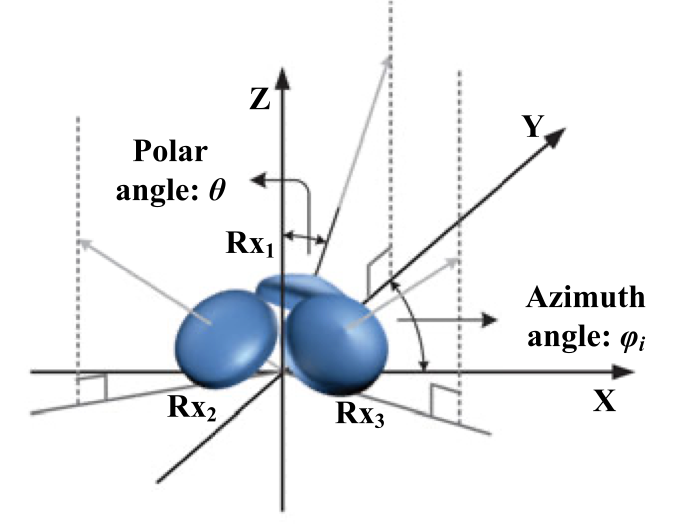
\includegraphics[width=8cm]{ch2pic/config_orient.png}
            \caption{文獻\cite{case:3d_layers}各PD於同一位置的擺設}
            \label{pic:config_orient}
        \end{figure}

        
        \qquad
        現今幾乎所有幾何方法的PD組態都是此種類型\cite{survey_light2018}。通過此限制,式\ref{eqn:model_no_lamb}可進一步簡化為式\ref{eqn:model_config_restrict}。

        \begin{equation}
            \label{eqn:model_config_restrict}
            \begin{aligned}
                &\text{Let }
                ^P\boldsymbol{P}_p=
                \left[\begin{array}{ccc}0&0&0\end{array}\right]^T
                \text{ for } p = 1,2,...,P\\
                &\text { If } Ie_{lp}<S ,\text{ then }Ie_{lp} \\
                    &= \frac{ReAPt}{ \pi}
                \frac{
                        {( ^{P}\boldsymbol{V}_p \cdot 
                            (
                                ^{PL} \boldsymbol{Ro}^{P}\boldsymbol{P}_l
                                + ^{PL}\boldsymbol{T}
                            )
                        )}
                {
                            (
                                -^{PL}\boldsymbol{Ro}^{L}\boldsymbol{V}_l 
                                \cdot 
                                (
                                    ^{PL}\boldsymbol{Ro}^{P}\boldsymbol{P}_l
                                    +^{PL}\boldsymbol{T}
                                )
                            )
                        } } 
                    {
                        {
                            ||
                                ^{PL}\boldsymbol{Ro}^{P}\boldsymbol{P}_l+^{PL}\boldsymbol{T}
                            ||
                        }^{4}
                    }\\
            \end{aligned}
        \end{equation}

        \qquad
        除了位置的限制,PD指向在文獻中也常將兩自由度降至一個自由度,也就是將$^P\boldsymbol{V}_p^{sph}$的方位角平均分配:$^P\beta_p = 2\pi/P$,而各PD的天頂角則限制為相同:$^P\alpha_p = ^P\alpha$,圖\ref{pic:config_orient}便屬於此種。在此限制下,$P$個PD擺設的自由度由$P\times5$各自由度降低至只剩一個變數:$^P \alpha$天頂角,使用此限制的文獻包含\cite{case:cart2d}\cite{case:cart3d}\cite{case:3d_layers}等。另外一種常見的擺設方法則是將上述擺法加上一個於中間的PD,如\cite{case:ml}。

        \item[$\cdot$ 限制定位維度]\hfill
        
        \qquad 
        現今使用幾何方法的LED與PD系統,大多定位維度僅到二維\cite{survey_light2018},將欲解的相對位置$^{PL}\boldsymbol{T}=\left[\begin{array}{ccc}^{PL}t_x&^{PL}t_y&^{PL}t_z\end{array}\right]^T$中的$^{PL}t_z$限制為已知,如圖\ref{pic:case_parallel}。由於大多LED與PD的定位系統使用室內原有的光源,因此此限制代表的意義,便是目標物僅能於室內地面的水平高度移動,垂直距離已知,無法定位不在地面上的目標物。此限制在數學模型上的意義,則是將相對位置欲解的變數由三個減少為兩個。

        \begin{figure}[htpb]
            \centering
            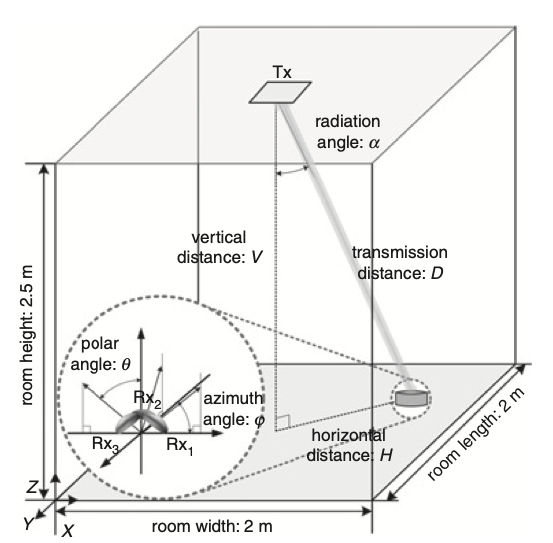
\includegraphics[width=10cm]{ch2pic/case_parallel.png}
            \caption{室內限制垂直距離的LED與PD定位系統架設\cite{case:aoa}}
            \label{pic:case_parallel}
        \end{figure}
        
        \qquad
        少數達到三維定位的LED與PD定位系統,大多是利用指紋法\cite{case:ml},然而指紋法為環境對單點的定位,不符合本研究需求。利用幾何方法達到三維定位的研究較少,其中\cite{case:cart3d}透過一已知$x,y$位置的參考點,來進行垂直距離的計算;\cite{case:3d_layers}則是使用複雜的演算法,利用迭代計算垂直距離;\cite{case:hypercube}則需使用兩平行且之間有距離的LED,利用PD兩兩比較電流大小,計算出三維相對位置;以上三篇研究皆有限制使用情境,而這些研究於\ref{chp:LEDPD_case}章詳述。



        \item[$\cdot$ 限制接收與發射平面平行]   \hfill
        
        \qquad
        在使用幾何類型演算法的研究中,常限制Step2.系統設置時,兩次系統的目標平面與量測者平面需平行,也就是LED與PD次系統座標系中的Z軸恆需平行,如圖\ref{pic:case_parallel}所示。舉例來說,展場內的光源中心軸朝地面,此時利用手機前鏡頭進行定位的使用者,便需將手機平放,以使其中心軸垂直地面朝上達到平行。

        \qquad
        透過此限制,光傳遞模型中的出射角$\theta$必與入射角$\phi$相等或是相關,即可將光傳播模型的變數降低至兩個,利用$\cos\theta=\cos\phi$可將式\ref{eqn:model_config_restrict}簡化至式\ref{eqn:model_parallel_restrict},其中的$^{PL}\boldsymbol{Ro}$也僅剩一個自由度,大大的簡化了模型複雜度。


        \begin{equation}
            \label{eqn:model_parallel_restrict}
            \begin{aligned}
                &\text { If } Ie_{lp}<s ,\text{ then }Ie_{lp} \\
                    &= \frac{ReAPt}{ \pi}
                \frac{
                        {( ^{P}\boldsymbol{V}_p \cdot 
                            (
                                ^{PL} \boldsymbol{Ro}^{P}\boldsymbol{P}_l
                                + ^{PL}\boldsymbol{T}
                            )
                        )}^2
                    } 
                    {
                        {
                            ||
                                ^{PL}\boldsymbol{Ro}^{P}\boldsymbol{P}_l+^{PL}\boldsymbol{T}
                            ||
                        }^{4}
                    }\\
            \end{aligned}
        \end{equation}

        \qquad
        雖然此限制常見,但是也造成很大的使用不便,除了室內光源搭配於地面上不改變垂直距離的移動載具以外,基本上沒有其他應用場域,大幅度限制了使用的情境,難以達到具有靈活度的應用,因此本研究的主要目標之一便是去除此限制。
    

    \end{description}
    






    \subsubsection{LED與PD定位系統文獻案例}
    \label{chp:LEDPD_case}

    

    \begin{table}[htpb]
        \begin{center}
          \caption{比較與本研究相似的文獻}
          \label{tab:LEDPD_case}
          \begin{tabular}{c||c|c|c|c|c} 

             文獻 &
              \textbf{目標物與量測者}&
              \textbf{定位}&
              \textbf{定位}& 
              \textbf{硬體}&
              \textbf{備註}\\

             & \textbf{平面平行}&\textbf{維度}&\textbf{範圍(m)}&\textbf{驗證} &\\
            \hline
            
            % \cite{case:hypercube}&
            % 限制&
            % 三維&
            % $0.5\times 0.5\times 0.3$&
            % 有(紅外光波段)\\
            
            \cite{case:3d_layers}&
            限制&
            三維&
            $2\times 2\times 2.5$&
            有&
            演算法迭代執行\\
            
            \cite{case:cart3d}&
            限制&
            三維&
            $1\times 1\times 1.5$&
            無&
            需有參照高度的參考點\\

            \cite{omg_new}&
            \textcolor{red}{不限制}&
            二維&
            $20\times 20\times 10$&
            無&
            \\

            % 本研究&
            % \textcolor{red}{不限制}&
            % 三維&
            % $3\times 3\times 3$&
            % 無&
            % \\
          \end{tabular}
        \end{center}
      \end{table}

      本段落將對介紹現行LED與PD文獻實例,其中針對本研究中單點對單點定位、兩次系統可自由移動定位的這些目標,篩選出幾篇與本研究目標較為接近的文獻舉例介紹,文獻特色呈現於表\ref{tab:LEDPD_case},根據是否限制目標物與量測者平面平行、定位維度、定位範圍、是否有硬體驗證等特性分類,並於以下進行分項介紹各文獻的細節與特色。

    \begin{description}
        % \item[\cite{case:hypercube}:使用紅外光且易於攜帶但量測範圍小的案例]\hfill 
        
        % \qquad
        % \cite{case:hypercube}研究利用2個LED與3個PD進行光通訊,光通訊流程如圖\ref{pic:vlc_flow},其將朗博次方假設為一,使用與圖\ref{pic:config_orient}相同的PD組態,實體圖為圖\ref{pic:hypercube_pd},為達到三維定位而限制目標物與量測者需為平行。

        % \begin{figure}[h]
        %     \centering
        %     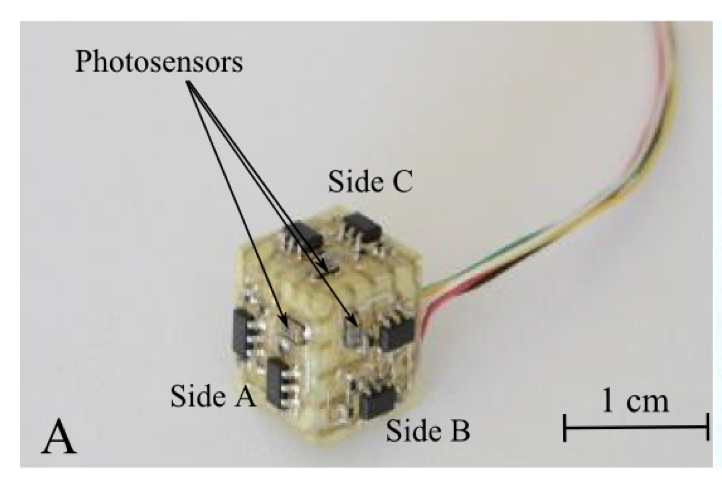
\includegraphics[width=6cm]{ch2pic/hypercube_pd.png}
        %     \caption{\cite{case:hypercube}的PD組態}
        %     \label{pic:hypercube_pd}
        % \end{figure}
        % \begin{figure}[h]
        %     \centering
        %     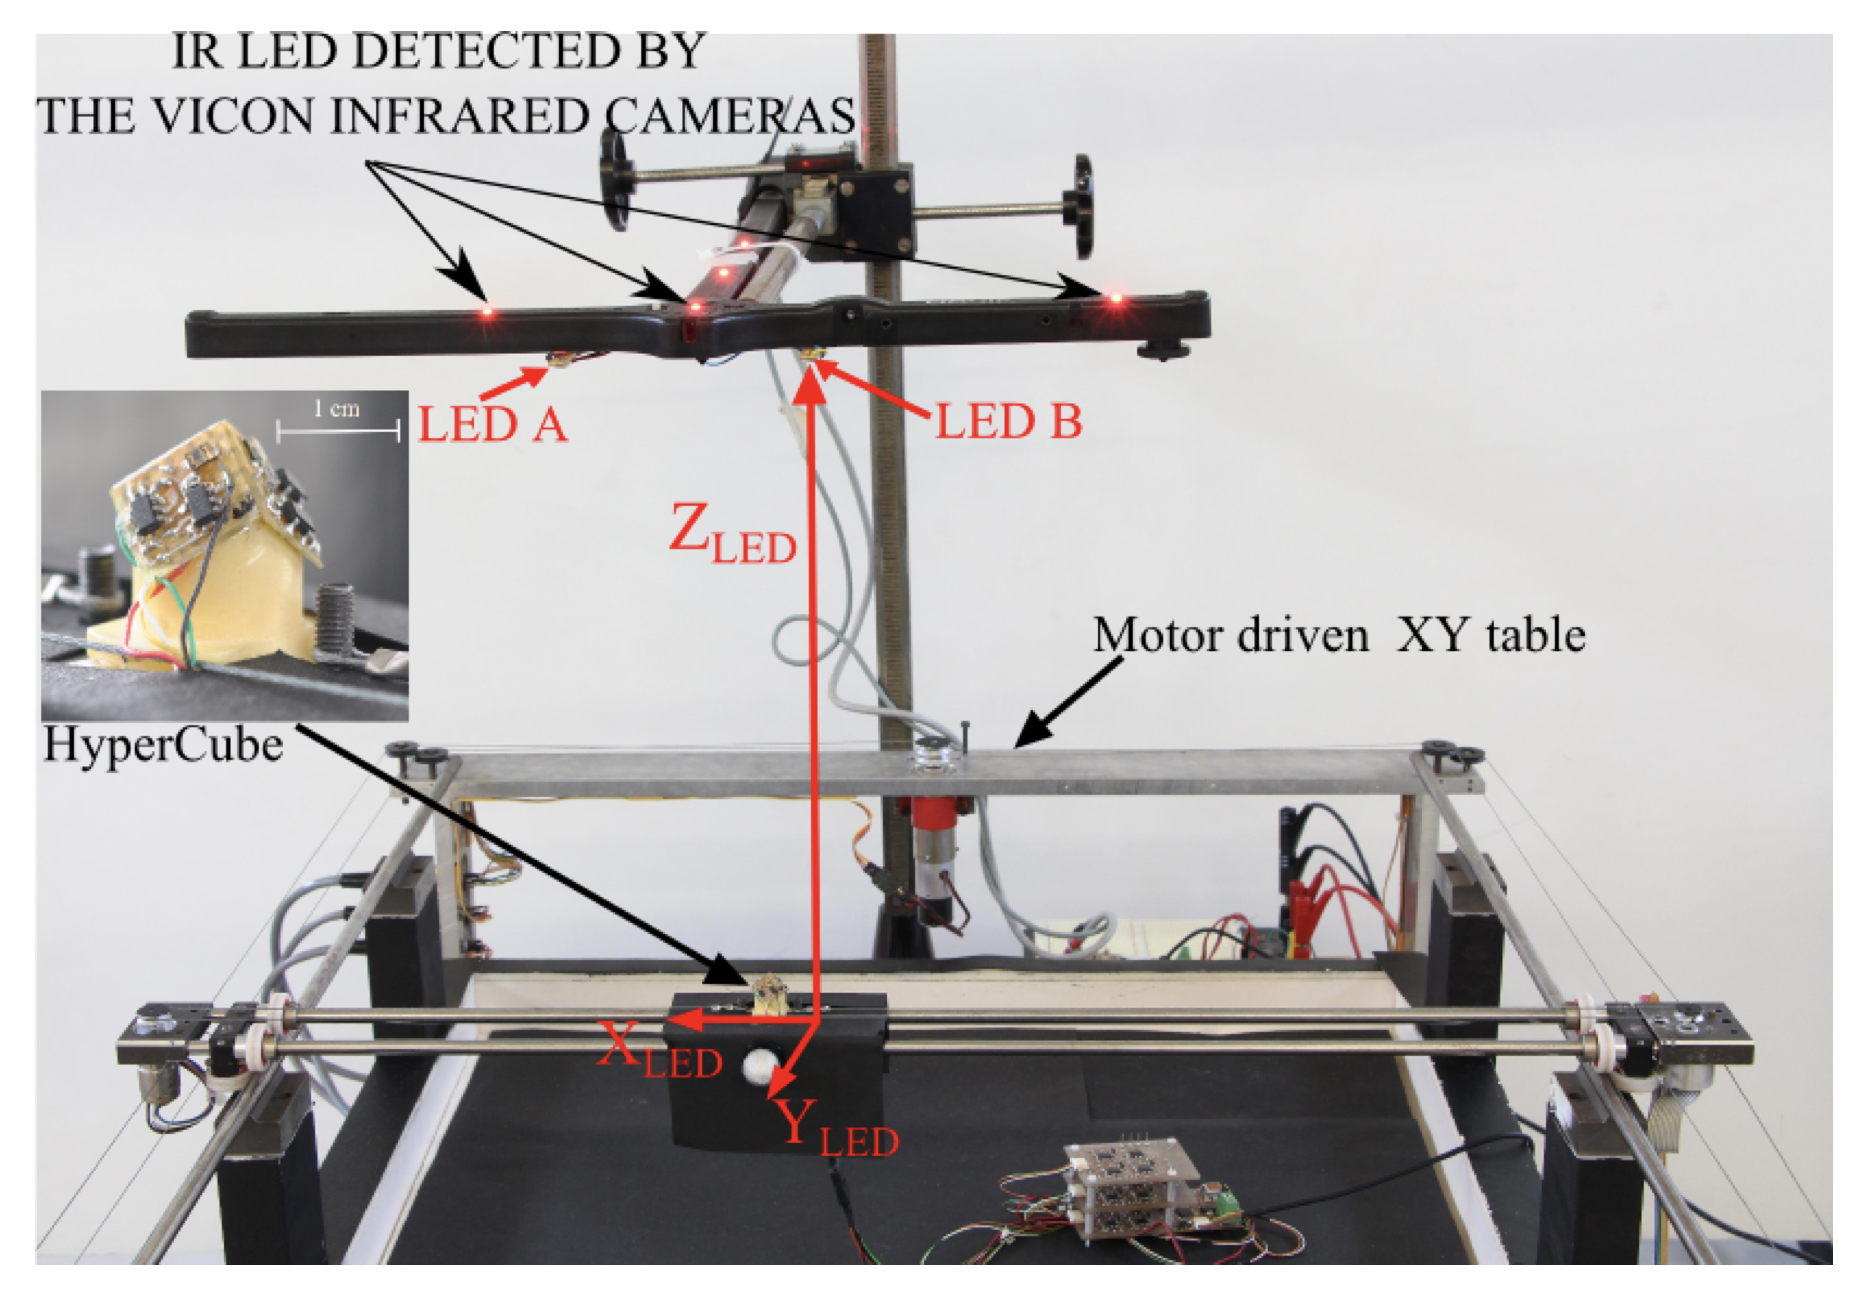
\includegraphics[width=9cm]{ch2pic/hypercube_setup.png}
        %     \caption{\cite{case:hypercube}的系統架構}
        %     \label{pic:hypercube_setup}
        % \end{figure}
        


        % \qquad
        % 簡單介紹此研究使用的演算法:首先,三個PD指向分別為:
        
        % $$^P\boldsymbol{V}_1=[1,0,0]^T,^P\boldsymbol{V}_2=[0,1,0]^T,^P\boldsymbol{V}_3=[0,0,1]^T$$
        
        % 因此,當只考慮一LED時,PD入射角餘弦分別為:
        % $$\cos\phi_{l1} = t_x/t_d,\cos\phi_{l2} = t_y/t_d,\cos\phi_{l3} = t_z/t_d$$
        
        % 而方位角$t_\beta = \arctan(t_y/t_x) = \arctan(\cos\phi_{l2}/\cos\phi_{l1})=Ie_{l2}/Ie_{l1}$。至於天頂角,此論文則是利用多項假設,例如假設$\cos\omega=\omega$以及$\cos(\omega+\pi/4)+\cos(\omega-\pi/4)=1$等條件,來使天頂角可透過$Ie_{l3}$獲得。有了出入射角之後,三維定位的部分是透過兩個放置距離已知的LED,如圖\ref{pic:hypercube_2led},利用AOA方式距離$t_d$,值得注意的是,兩LED距離越大可提高精度,但也同時會變成環境對單點的定位,不符合本研究目的。

    

        % \begin{figure}[h]
        %     \centering
        %     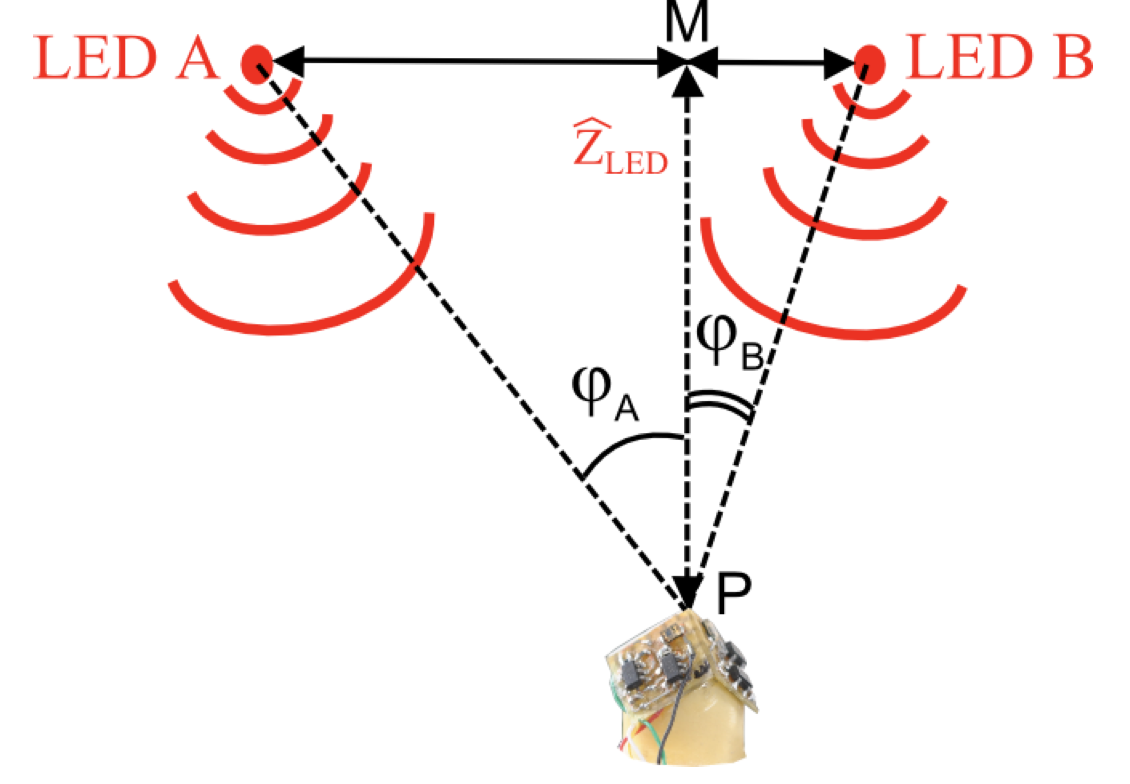
\includegraphics[width=7cm]{ch2pic/hypercube_2led.png}
        %     \caption{\cite{case:hypercube}利用兩個LED達到三維定位}
        %     \label{pic:hypercube_2led}
        % \end{figure}
        
        % \qquad
        % 此研究針對僅有$50\times 50mm$的範圍,垂直距離也僅有$300mm$,範圍非常小;而實驗中二維定位可達到平均誤差為1.6mm的精度,垂直距離的誤差最大來到50mm。該研究值得注意的是,他將PD封裝成一非常小的單位,完全符合易攜帶又成本低的特色,並進行實體系統的搭建與實驗。除此之外,其利用的波段為紅外光,為少數不利用可見光與室內現成光源的LED與PD系統,使LED與PD定位不侷限於室內照明光源的應用上。




        \item[文獻\cite{case:3d_layers}:迭代獲得三維定位的案例] \hfill 
        
        \qquad
        本研究的系統架構如圖\ref{pic:env_1to1},利用單個LED與三個PD達到三維定位並進行實際硬體系統搭建與驗證,測試範圍為$2\times 2\times 2.5m$,不考慮朗博次方,而PD擺設如圖\ref{pic:config_orient},屬於\ref{chp:LEDPD_restrict}章中PD次系統最常見的擺設限制,除此之外也需限制目標平面與量測平面平行。
        
        \qquad
        此文現在Step4.執行定位演算法的部分,是將PD電流兩兩相除為入射角的餘弦比值,如式\ref{eqn:hypercube},當相對位置中的z分量$^{PL}t_z$為已知特定值時,餘弦比值呈現於圖\ref{pic:layers_2d},任兩PD可獲得一$^{PL}t_x,^{PL}t_y$與餘弦比值的關係圖。因此,PD兩兩計算訊號強度比值,各強度比值可於圖\ref{pic:layers_2d}中的子圖取得一條代表$^{PL}t_x,^{PL}t_y$可能位置的線段,三條線段交點即為二維定位的解$t^{PL}_x,^{PL}t_y$,其中,實驗中平均誤差小於3cm。三維定位的部分,則是將量測空間垂直距離每十公分切為一層如圖\ref{pic:layers_3d},每層皆利用上述二維定位的方法計算一次$^{PL}t_x,^{PL}t_y$,再將該位置$^{PL}t_x,^{PL}t_y$與利用光傳遞模型計算出各PD理論上該得到的電流值$Ie_{lp}$,將計算出的電流與實際PD電流比對,最接近的該層則為三維定位的垂直距離。

        \begin{equation}
            \label{eqn:hypercube}
            \begin{aligned}
                    \frac{Ie_{11}}{Ie_{12}}= 
                \frac{
                    ( ^{P}\boldsymbol{V}_1 \cdot 
                    ^{PL}\boldsymbol{T}
                    )
                } 
                    {
                        ( ^{P}\boldsymbol{V}_2 \cdot 
                                ^{PL}\boldsymbol{T}
                        )
                    }=\frac{\cos\phi_{11}}{\cos\phi_{12}}
            \end{aligned}
        \end{equation}

        \begin{figure}[htpb]
            \centering
            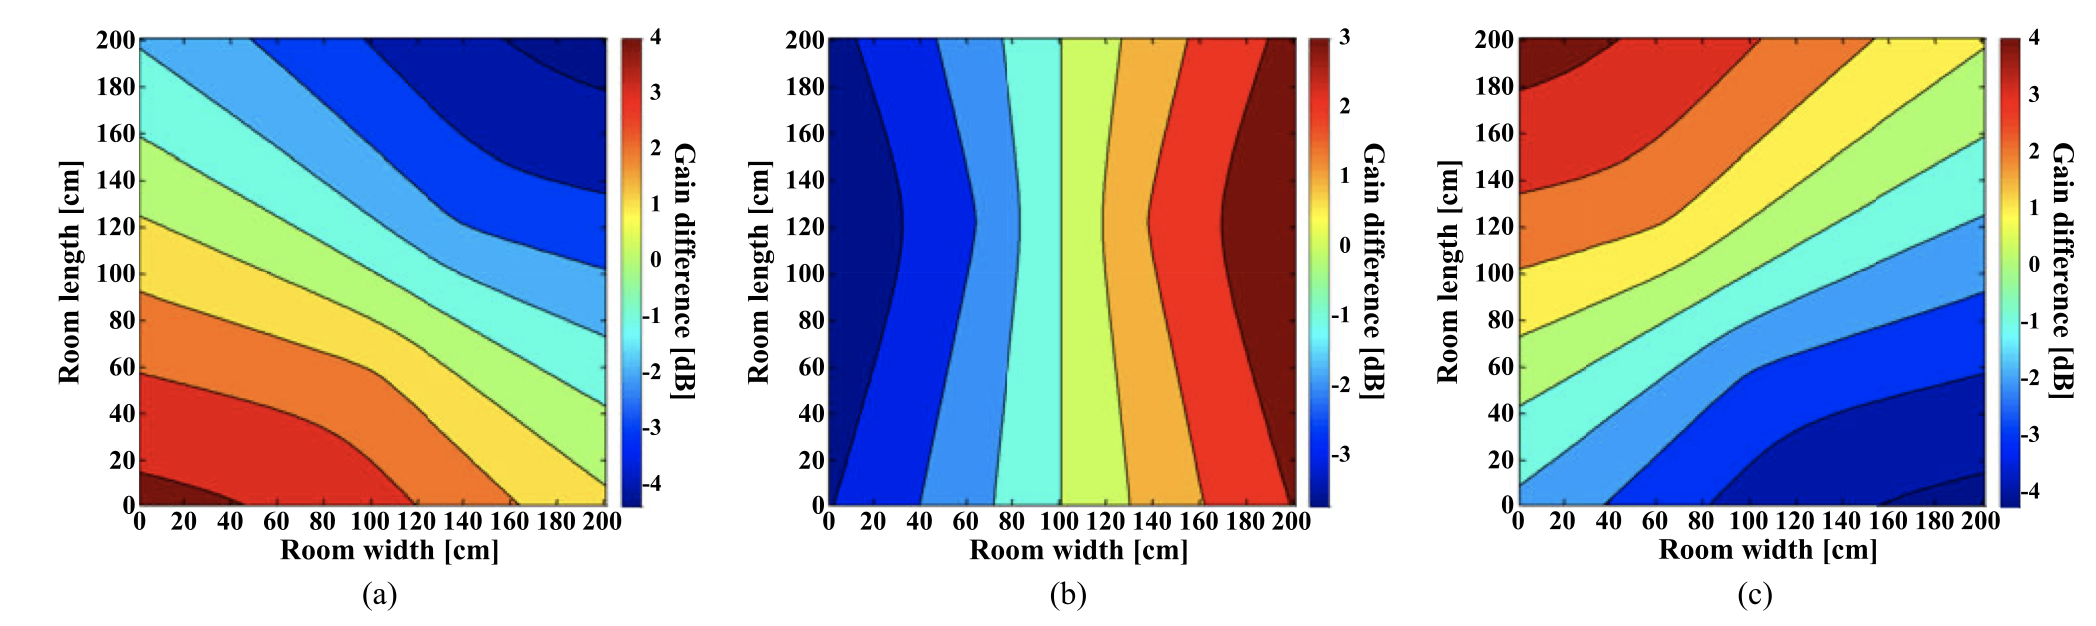
\includegraphics[width=15cm]{ch2pic/layers_2d.png}
            \caption{文獻\cite{case:3d_layers}中地面上PD電流強度比值(a)第一與第二個PD(b)第二與第三個PD(c)第一與第三個PD}
            \label{pic:layers_2d}
        \end{figure}

        \begin{figure}[htpb]
            \centering
            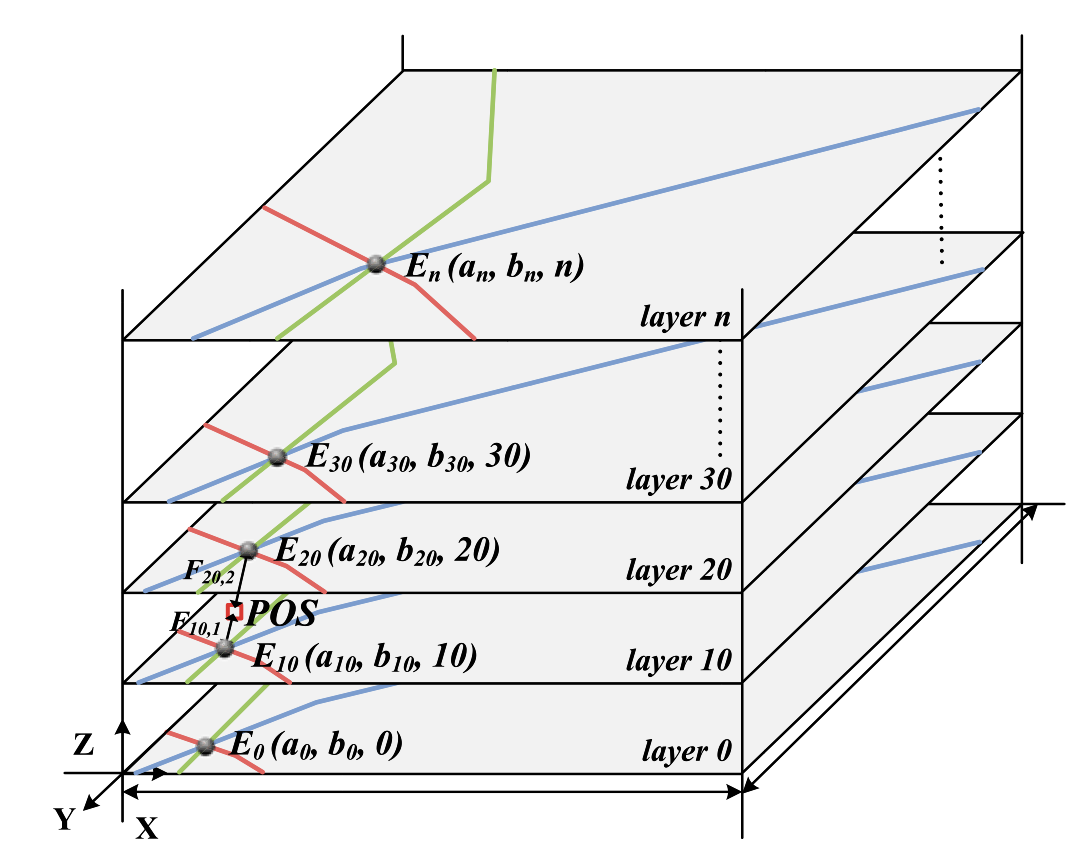
\includegraphics[width=12cm]{ch2pic/layers_3d.png}
            \caption{文獻\cite{case:3d_layers}中將量測空間切為多層}
            \label{pic:layers_3d}
        \end{figure}

        \qquad
        此方法特殊在其利用與絕大多數研究相同的系統架構,卻透過特殊的演算法,利用迭代量測空間中不同高度的各層,計算該層理論上應量測到的PD電流大小與實際量測的電流大小差異,以進行三維定位。除此之外,該文獻有進行實驗驗證,屬於少數搭建實際硬體系統的文獻。然而,該方法在垂直距離的定位,解析度為迭代每層高度之間的距離10cm,若要達到更高的解析度則需要切更多層,而在迭代且取最小值的演算法已經十分耗時的狀況下,切更多層更會加大運算負擔。



        \item[文獻\cite{case:cart3d}:事先校正參考點以獲得三維定位的案例] \hfill 
        
        \qquad
        本研究架構與PD組態於圖\ref{pic:case_cart3d},其利用單LED與五個PD,量測範圍為$1\times 1\times 1.5m$,限制則一樣是目標平面與觀察平面需平行,而朗博次方則是有考慮LED的朗博次方,PD的朗博次方則忽略視為一。
        
        二維定位的方法也是利用兩兩PD的電流比值,透過已知的PD組態回推目標物的方位,模擬達到平均$2.32cm$的經度。垂直距離則需要透過一參考點,該參考點需與目標物的垂直距離相同且已知方位,即可透過與參考點比較得到目標物的垂直距離,而模擬中達到平均$5.08cm$的精度。

        \begin{figure}[htpb]
            \centering
            \includegraphics[width=12cm]{ch2pic/case_cart3d.png}
            \caption{文獻\cite{case:cart3d}的(a)系統架構(b)PD組態}
            \label{pic:case_cart3d}
        \end{figure}

        \qquad
        該研究特色之一為其考慮了LED的朗博次方,而演算法則相較簡單,透過幾何關係計算且具有實驗驗證。雖然該研究成功獲得三維定位,但卻需要有一同樣垂直距離的參考點,使得應用情境仍受限制;若移動、改變垂直距離則參考點作廢,需重新量測參考點,使用情境上受限。



        \item[文獻\cite{omg_new}:不限制平面平行的二維定位方法]\hfill
        
        \qquad
        此系統由三個LED與一個PD組成,透過軟體模擬,分析於$10\times 10\times 10$公尺範圍內的定位成效。該系統使用的限制包含不考慮PD朗博次方、需已知相對位置的z分量$^{PL}t_z$、LED擺設於同一位置等。

        \qquad
        該系統在Step4.執行二維系統演算法的部分,則與上述兩例子相似,由於三個於同位置的LED至同一PD,在幾何交互關係中距離與PD入射角皆相同,因此透過訊號比值可獲得LED出射角的餘弦比值,與\ref{eqn:hypercube}相似。而由餘弦比值獲得相對位置中的方位$^{PL}\boldsymbol{Tv}$,則是將任兩LED餘弦比值換算為相對方位$^{PL}\boldsymbol{Tv}$與LED指向內積$^{PL}\boldsymbol{V}_l$,如下式\ref{eqn:omg},透過三個LED中三組餘弦比值來解聯立求得方位。
        
        \begin{equation}
            \label{eqn:omg}
            \frac{\cos\theta_{11}}{\cos\theta_{21}}=\frac{^{PL}\boldsymbol{Tv}\cdot^{PL}\boldsymbol{V}_1 }{^{PL}\boldsymbol{Tv}\cdot^{PL}\boldsymbol{V}_2 }
        \end{equation}

        \qquad
        本文獻的主要特色在於其不需限制量測者與目標物平面平行,然而其並無法取得三維定位,因此在使用情境上仍十分受限,並不符合本研究目標。
        
        

    \end{description}

    \hfill

    以上介紹了LED與PD系統中,三篇利用單點對單點的系統架構進行定位的方法。其中,各自使用的限制與演算法不同,但並沒有一同時可以不限制目標物與量測者平面平行、考慮朗博次方並可達到三維定位的方法,仍無法滿足本研究目標。




\subsection{現行LED與PD定位所遇困難}
\label{chp:LEDPD_problem}
    
綜合\ref{chp:LEDPD_restrict}章中敘述的限制與案例,以下統整,分項探討此領域所欠缺的面向。

\begin{description}

    \item[- 系統限制多]\hfill 
    
    \qquad
    如\ref{chp:LEDPD_restrict}章所述,常見的限制包含忽略朗博次方的影響、限制硬體選擇、限制PD組態、限制定位維度、限制使用情境等。當一次使用所有限制,即可得到式\ref{eqn:model_parallel_restrict}中簡單的模型,能夠輕易的取得相對定位。然而如\ref{chp:LEDPD_restrict}章所述,忽略朗博次方不符合實際情況,而其他的限制都會限制系統靈活度,也就是本論文最主要的目標,因此提出一限制較少的定位演算法有其必要性。
    
    \item[- 較少硬體實驗驗證]\hfill 
    
    \qquad
    在LED與PD系統中的研究,大多僅使用模型模擬,實際架設硬體進行實驗的案例較少,於\cite{survey_light2018}中整理的35個研究中,僅有不到一半的研究有進行實驗,其中\cite{case:hypercube}\cite{case:3d_layers}為有進行硬體實驗的少數研究。大多研究不進行實驗驗證的原因,其中之一為光通訊相較無線電波為較新的技術,LED光通訊在2000年被提出\cite{vlc},因此光通訊的硬體搭建並不像發展超過百年的無線電波技術完全,光通訊使用的驅動器與LED尚未被組合並商品化\cite{vlc_adv},相較無線電播技術中觸手可及的硬體,系統架設難度較高。因此大多研究先透過模擬,探索演算法與不同系統組態的可能性,具有架設完整光通訊系統能力的實驗室才會進一步進行實驗。


    \item[- 忽略誤差]\hfill 

    \qquad
    首先,最常被忽略的是多重路徑傳輸(圖\ref{pic:multipath})所產生的誤差,因為多重路徑傳輸與環境、障礙物的位置與材質皆相關,十分複雜,而該誤差於障礙物附近最為嚴重,如室內的角落。實驗上,經常將測試範圍選擇於一空曠廣大的室內中心,將測試範圍與牆壁的距離拉開,減少多重路徑傳輸效應。而僅進行模擬的研究中,模擬多重路徑誤差的難度很高\cite{multipath},三維空間中要判斷透過多次反彈能夠到達PD的光束,計算非常複雜,且針對具有障礙物等較為複雜的環境,多重誤差的模擬則更為複雜,

    再來,光定位中另一個造成誤差主要原因為環境光源,實際上在光通訊系統中,由於環境光源並不會閃爍,因此可透過將偏差(Bias)去除,以此處理環境光源。然而環境光源仍有可能使PD電流超過飽和,因此常見處理方式為將系統架設於無窗戶之室內,模擬上則常常直接將其忽略。

\end{description}






\section{結論}
\label{chp:2_conclusion}

利用LED與PD的技術且使用幾何方法類型演算法的文獻,由於光傳遞模型變數除了距離還有出入射角,具有靈活應用的潛力,近年來開始被討論。然而,此領域有以下不足:常見的系統限制多、較少硬體實驗驗證、以及忽略誤差。本研究目標為靈活應用,因此主要著重於減少系統限制,\ref{chp:LEDPD_restrict}章中敘述的限制中,本論文目標將朗博次方完整考慮,並解決使用情境與定位維度的限制。

因此,本研究主要針對部分缺點進行改進:首先,本研究將考量LED與PD的朗博次方,完整將硬體不同的輻射模式納入模型;另外,本研究於\ref{chp:3}章中提出一能夠達到三維定位,且不需限制目標物與量測者平行的演算法,以提升使用上的靈活度,達到兩單位自由移動且能定位的目標情境。
    


   %====================================================== 


    
    



        



        
        


        

    



        

        


